% Created 2023-08-15 Tue 10:49
\documentclass[9pt, b5paper]{article}
\usepackage{xeCJK}
\usepackage[T1]{fontenc}
\usepackage{bera}
\usepackage[scaled]{beraserif}
\usepackage[scaled]{berasans}
\usepackage[scaled]{beramono}
\usepackage[cache=false]{minted}
\usepackage{xltxtra}
\usepackage{graphicx}
\usepackage{xcolor}
\usepackage{multirow}
\usepackage{multicol}
\usepackage{float}
\usepackage{textcomp}
\usepackage{algorithm}
\usepackage{algorithmic}
\usepackage{latexsym}
\usepackage{natbib}
\usepackage{geometry}
\geometry{left=1.2cm,right=1.2cm,top=1.5cm,bottom=1.2cm}
\usepackage[xetex,colorlinks=true,CJKbookmarks=true,linkcolor=blue,urlcolor=blue,menucolor=blue]{hyperref}
\newminted{common-lisp}{fontsize=\footnotesize} 
\author{deepwaterooo}
\date{\today}
\title{ET 框架学习笔记(四)--框架总结【爱表哥,爱生活!!!活宝妹就是一定要嫁给亲爱的表哥!爱表哥,爱生活!!!】【活宝妹坐等亲爱的表哥,领娶活宝妹回家!爱表哥,爱生活!!!】}
\hypersetup{
  pdfkeywords={},
  pdfsubject={},
  pdfcreator={Emacs 28.2 (Org mode 8.2.7c)}}
\begin{document}

\maketitle
\tableofcontents


\section{C\# 异步基础原理、状态机原理、逻辑整理}
\label{sec-1}
\subsection{ETVoid C\# Net-async|await 编程更底层一点儿的原理}
\label{sec-1-1}
\begin{itemize}
\item 就是不懂底层的原理是什么,方法定义是什么,返回的是什么,在有 await 等关键字的时候,返回的内容等是如何变换的,以及它背后的那个异步状态机,就是想不明白。
\item 现在参考网上的一个例子,记一下异步任务C\# 幕后封装的那些执行步骤什么的,把 async await 之类的关键字,背后的逻辑理解明白。
\item 就是,可能也可以在异步任务的这个模块,添加无数的日志,通过读日志来把这块儿弄明白。下面就截图网上的这个参考例子。
\begin{minted}[fontsize=\scriptsize,linenos=false]{csharp}
[AsyncMethodBuilder(typeof (AsyncETVoidMethodBuilder))]
internal struct ETVoid: ICriticalNotifyCompletion {
    [DebuggerHidden]
    public void Coroutine() { }
    [DebuggerHidden]
    public bool IsCompleted => true;
    [DebuggerHidden]
    public void OnCompleted(Action continuation) { }
    [DebuggerHidden]
    public void UnsafeOnCompleted(Action continuation) { }
}
\end{minted}
\item 上面是找了一个最短小的类ETVoid, 网上例子自己构建一个类,这个类麻雀虽小五脏俱全的 \textbf{几个【缺一不可】的方法} (所以知道ETTask|ETVoid 自定义封装,这几个方法也是一定不能少的,只是多了Coroutine() 方法不知道是怎么回事儿?)如上如下:
\end{itemize}

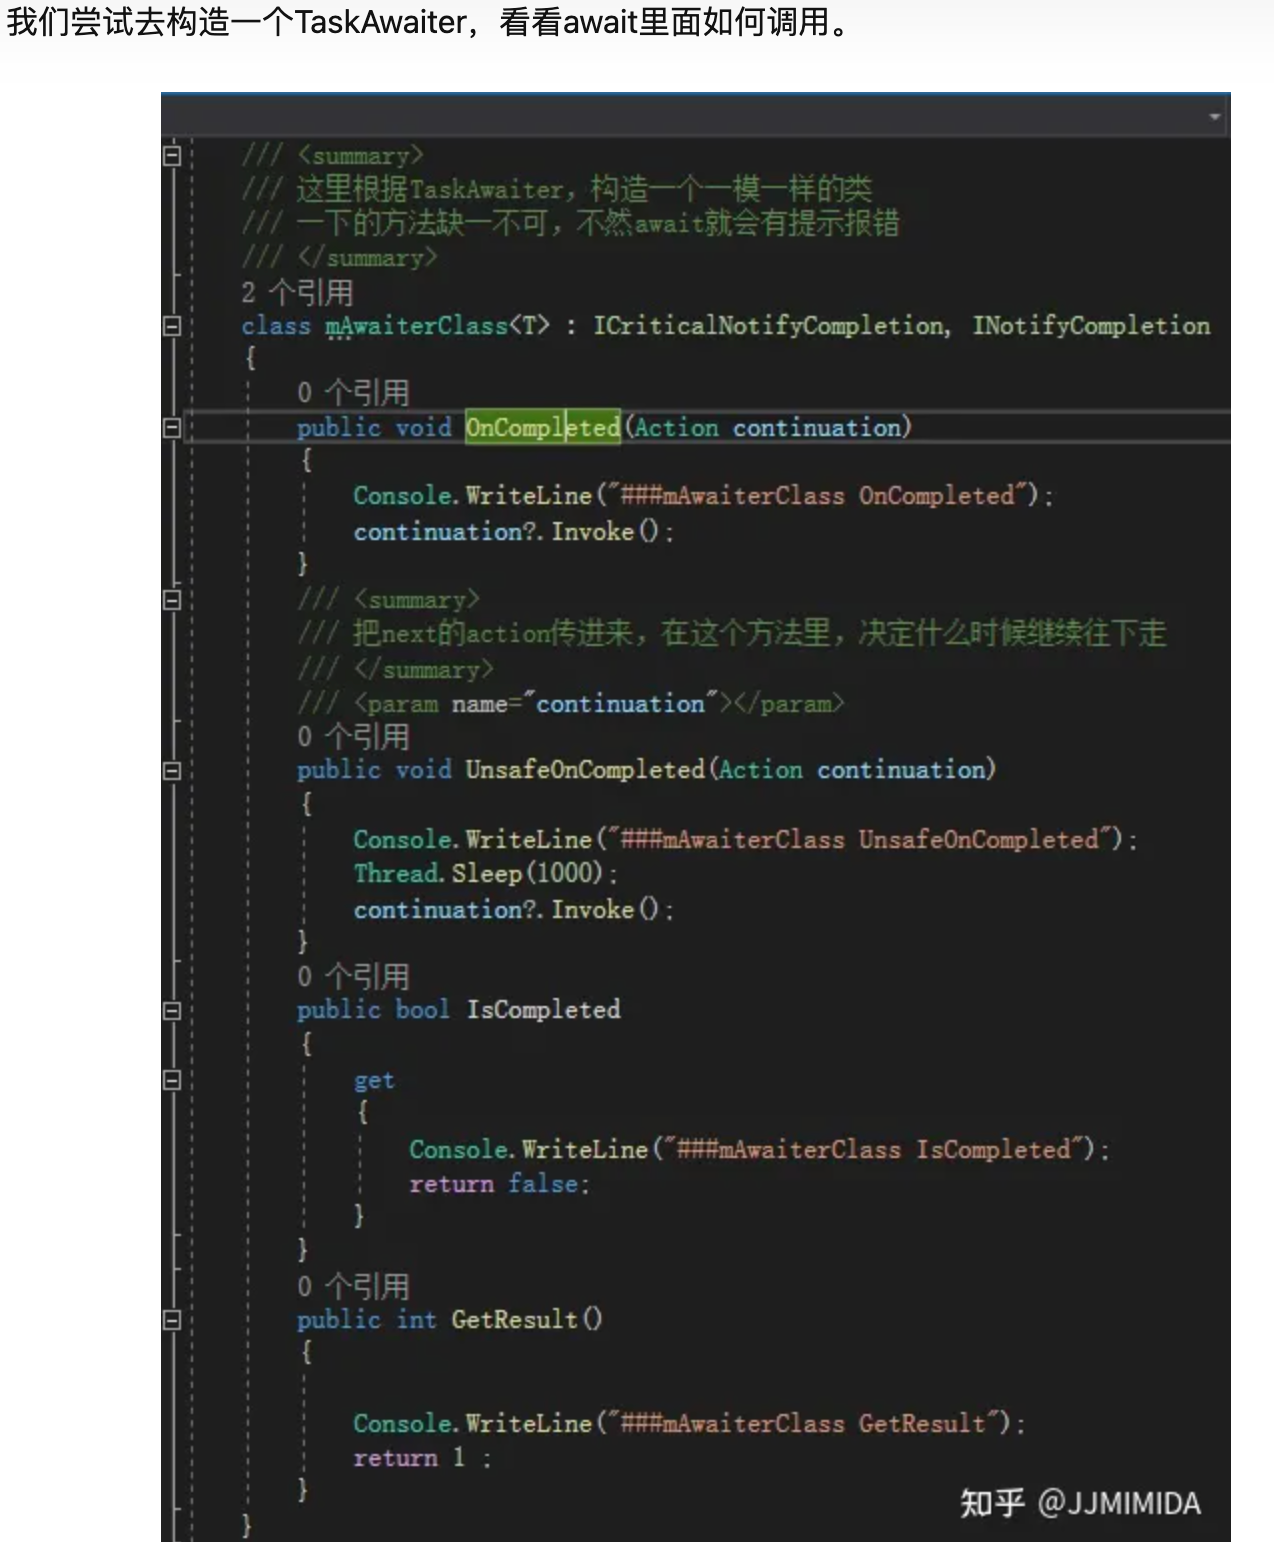
\includegraphics[width=.9\linewidth]{./pic/et3_20230609_105627.png}
\begin{itemize}
\item 它的测试用例是这么写的:注意它传入的参数类型是 int. 后面的编译码里,和它的讲解里会用到提到。
\end{itemize}

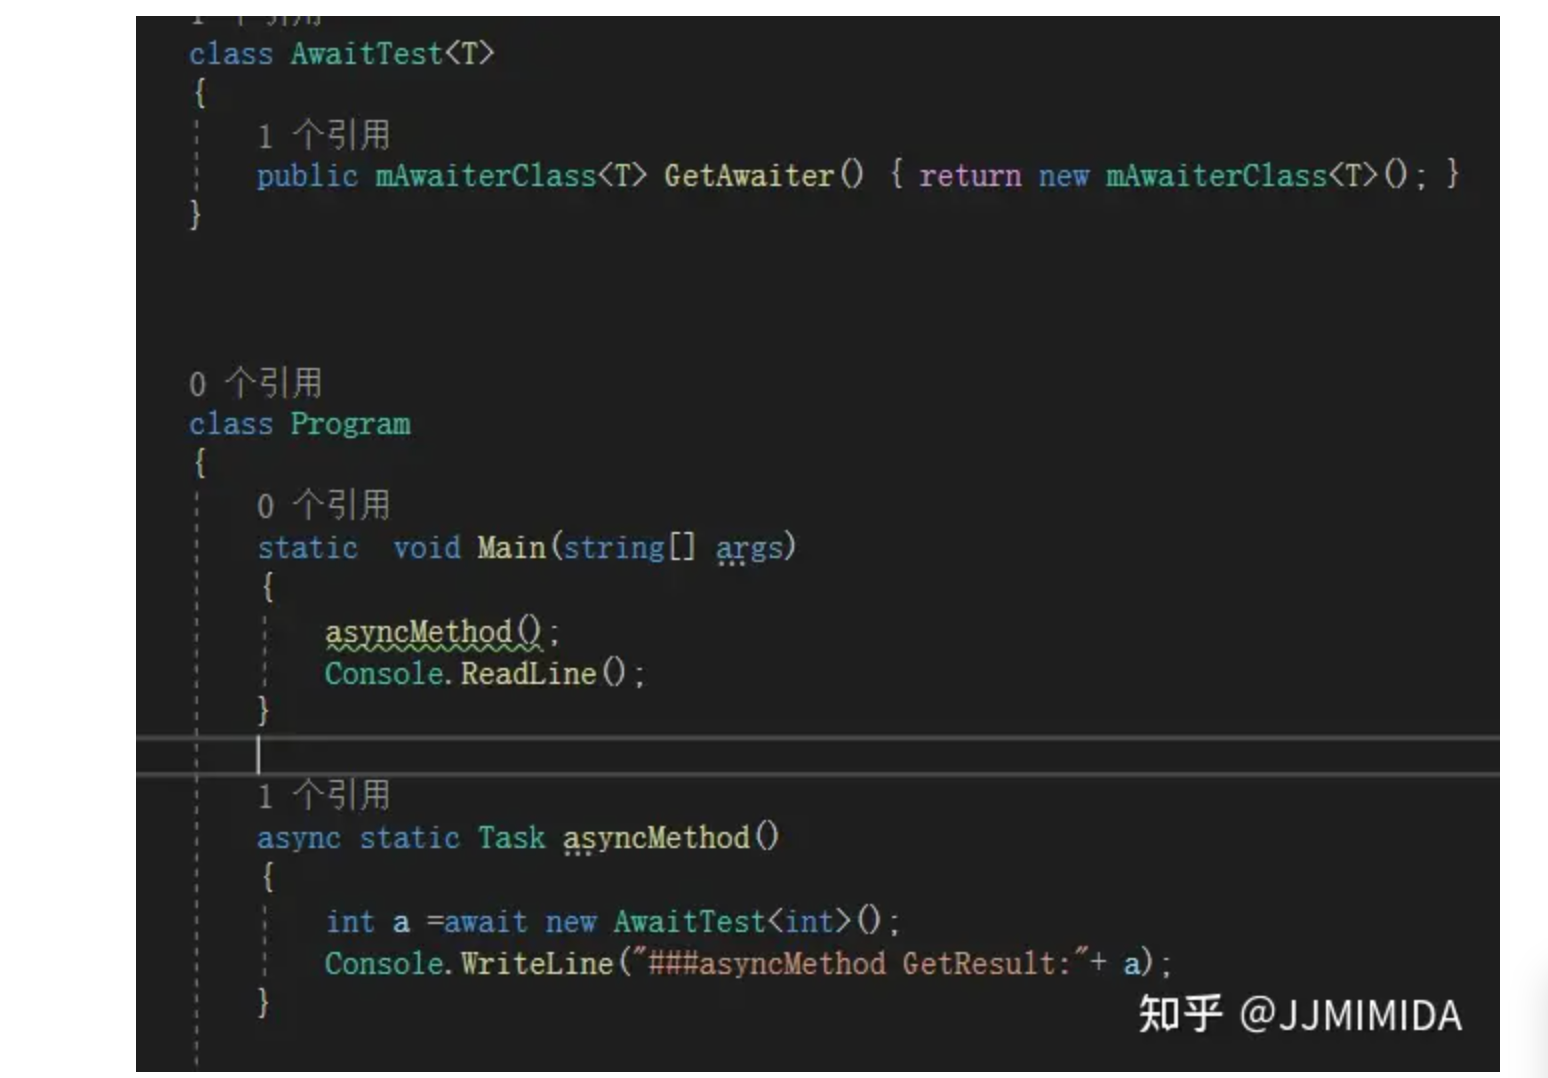
\includegraphics[width=.9\linewidth]{./pic/et3_20230609_105927.png}
\begin{itemize}
\item 看它编译出来的码(那堆编译出来的状态机的码),就是看不懂
\end{itemize}

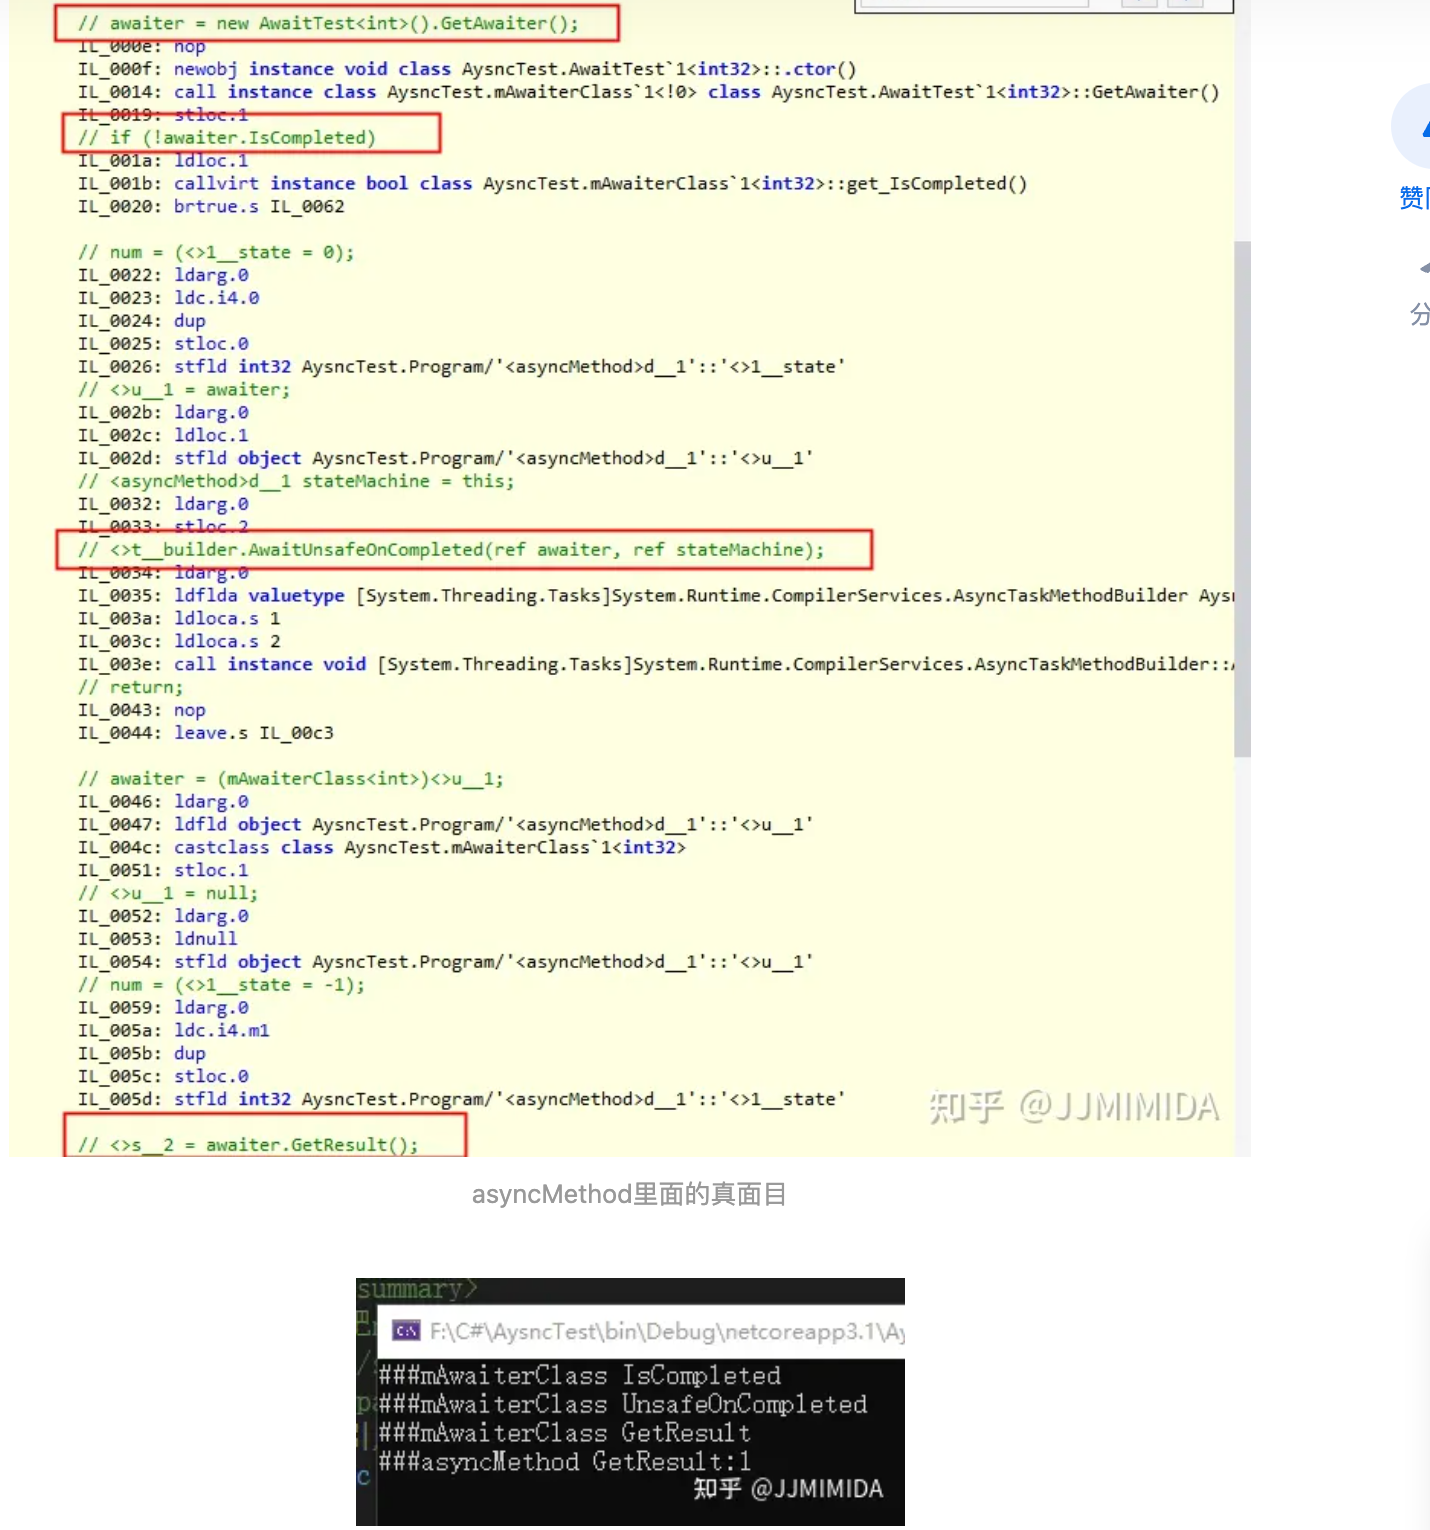
\includegraphics[width=.9\linewidth]{./pic/et3_20230609_112727.png}
\begin{itemize}
\item 结果分析: \textbf{【异步方法状态机,背后的执行顺序与逻辑:】}
\begin{itemize}
\item 先检查IsCompleted标志位,如果已经完成,则调用GetResult作为await的返回值返回。
\item 如果未完成,经过AsyncTaskMethodBuilder的AwaitUnsafeOnCompleted方法之后,最后进入UnsafeOnCompleted(nextAction),并且把完成后的下一步回调传进来。
\item 当我们获得nextAction之后,说明该调用由我们自己来控制,这里我在等待1s之后,执行nextAction(),下一步GetResult返回。
\end{itemize}
\item \textbf{【Async 关键字方法的编译原理:】}
\end{itemize}

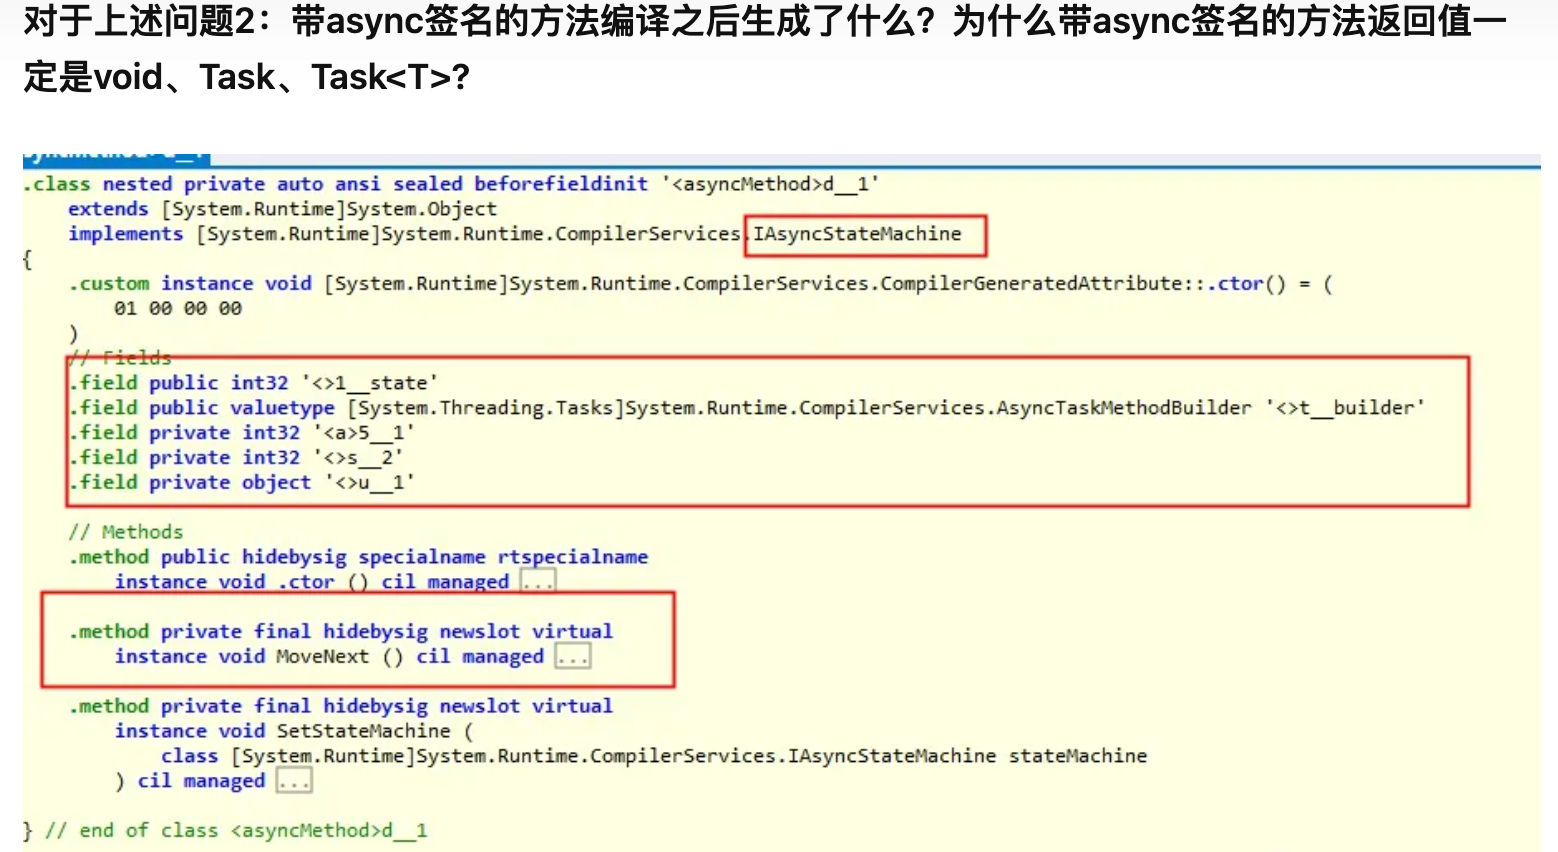
\includegraphics[width=.9\linewidth]{./pic/et3_20230609_110634.png}
\begin{itemize}
\item 这个 async 关键字所标记的异步方法,主要两个点儿: 
\begin{itemize}
\item 编译器,把这个异步方法,编译成了一个类 class <asyncMethod>d\_\_1;
\item 这个类 class, 它实现了 IAsyncStateMachine 接口,( \textbf{实现了这个接口,返回的是什么类型呢?} 这个要想明白?)
\item 这个类 class, 的内部,有几个成员变量 .field-sss.
\item 这个类 class, 的内部,有个特别重要的状态机执行函数 MoveNext() 来指挥指导,异步函数内不同节点如 await 节点等的执行逻辑。 \textbf{【这个类 class, 它实现了 IAsyncStateMachine 接口】}, 前面有列出 IAsyncStateMachine 接口定义的两个方法,所以实现实体类里也会有SetStateMachine() 方法的实现。
\item 上面的逻辑,其实是就是扫描异步方法内,不同的 await 调用,每到一个这个关键字申明的异步调用,就是切换一个状态(背后有可能是线程的切换, 不一定每个分支都用不同的线程,但线程的切换可能是,必要的时候需要切换的?)分段执行。
\end{itemize}
\item 网络上的分析者还给出了下机的截图:不是狠懂,这个截图是什么意思?因为不懂,要把编译码的方法名带上,方便以后再读和理解。
\end{itemize}

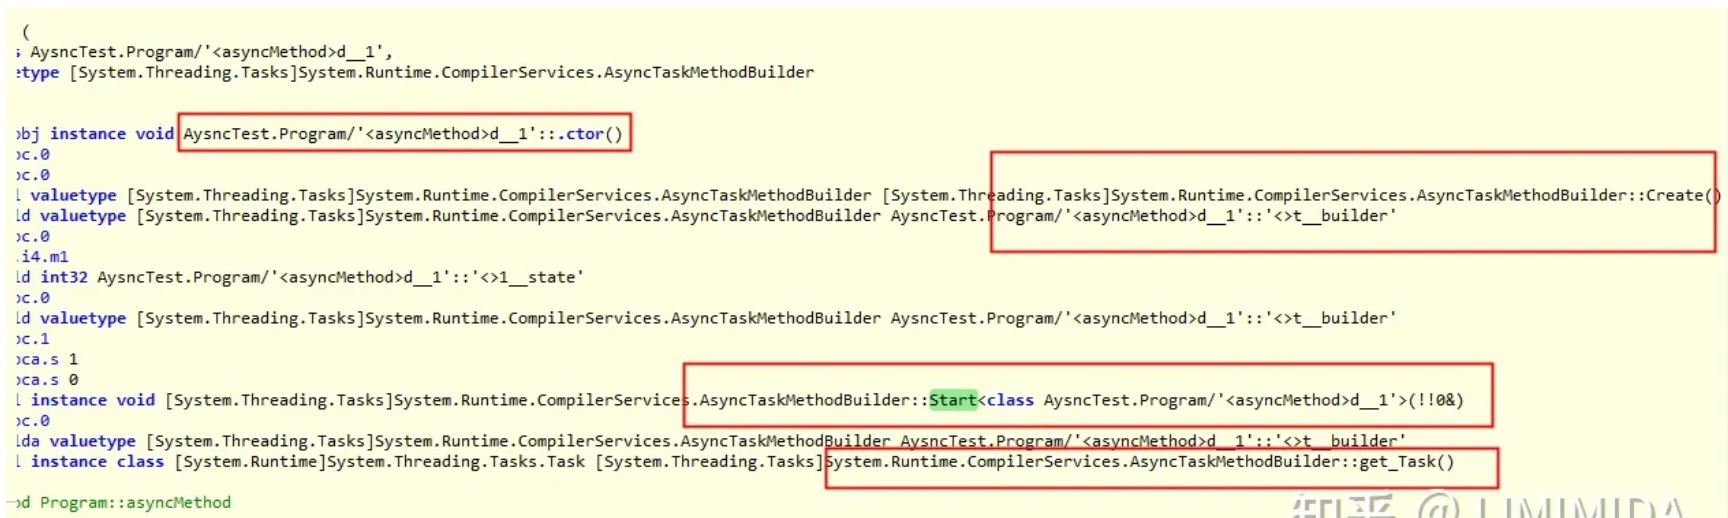
\includegraphics[width=.9\linewidth]{./pic/et3_20230609_112757.png}
\begin{itemize}
\item 上面的异步方法,所生成的异步状态机类 class 里,有几个主要的方法:
\begin{itemize}
\item 构造器方法 ctor():
\item Create() 方法:
\item Start() 方法:
\item get\_Task() 方法:
\end{itemize}
\item 可是上面的几个方法是谁,哪个接口定义的呢?
\item 网络上的分析者,对上面两个截图的分析如下: \textbf{【它讲解的这部分,我可能还是得自己编译一下,去具体看一下。】因为它的截图不完整,看不懂} 下面还有个别人总结的状态机套路,感觉说得更彻底透彻。
\begin{itemize}
\item 签名为async Task asyncMethod()的方法里,先创建一个继承自IAsyncStateMachine的asyncMethod类
\item 创建一个AsyncTaskMethodBuilder,然后赋值给Machine. (不知道,它这句,说的是哪里?第一个图的最后 SetStateMachine()?)
\item 初始化Machine的state = -1. (两个截图里看不见,找不到)
\item 调用AsyncTaskMethodBuilder.Start方法,start里面会进入Machine的moveNext()方法,详见问题1。
\item AsyncTaskMethodBuilder.get\_Task() 作为该方法的返回值返回。
\end{itemize}
\item 多线程问题: Task一定是多线程吗?
\begin{itemize}
\item 不一定,在上述例子中,我们定义的 async static Task<int> aa(),里面就是在同一个线程执行的。只有调用Task.Start 或者Task.Run 里面自动启用多线程的时候,才是多线程。
\end{itemize}
\item 看得另一个网页中的说法,因为感觉它也没有实现个什么公共定义约束的接口,理解得不够透彻。看下下面的:
\item await 必须配合 Task/ValueTask 才能用吗?当然不是。
\begin{itemize}
\item 在 C\# 中 \textbf{只要你的类中包含 GetAwaiter() 方法和 bool IsCompleted 属性,并且 GetAwaiter() 返回的东西包含一个 GetResult() 方法、一个 bool IsCompleted 属性和实现了 INotifyCompletion,那么这个类的对象就是可以 await 的} 。这里说得还是不清楚,不透彻,换一个表达得更清晰的说法如下:
\end{itemize}
\item 可以使用await的方法,返回值必须是 \textbf{awaitable对象} ,自定义awaitable对象比较麻烦,一个对象必须满足下列条件才行:
\begin{itemize}
\item 必须有一个 \textbf{GetAwaiter()} 方法,扩展方法或者实例方法都可以
\item GetAwaiter() 方法返回值必须是 \textbf{awaiter对象} 。一个对象要成为awaiter对象必须满足下列条件:
\begin{itemize}
\item 该对象 \textbf{实现接口 INotifyCompletion 或者ICriticalNotifyCompletion}
\item 必须有 \textbf{IsCompleted属性}
\item 必须有 \textbf{GetResult()方法} ,可以返回void或者其他返回值。
\end{itemize}
\end{itemize}
\item 比如下面的自定义类:把几个类的本质理解得再深一点儿了吗?【爱表哥,爱生活!!!任何时候,活宝妹就是一定要嫁给亲爱的表哥!!!】
\end{itemize}
\begin{minted}[fontsize=\scriptsize,linenos=false]{csharp}
public class MyTask<T> {
    public MyAwaiter<T> GetAwaiter() {// 必须提供的方法 
        return new MyAwaiter<T>();
    }
}
// 下面自定义的类 MyAwaiter<T=亲爱的表哥> 就是可以 await 的:
// 【任何时候,活宝妹就是一定要嫁给亲爱的表哥!!!活宝妹还没能嫁给亲爱的表哥,活宝妹就是永远守候在亲爱的表哥的身边!!!爱表哥,爱生活!!!】
public class MyAwaiter<T> : INotifyCompletion {// 必须实现的接口
    public bool IsCompleted { get; private set; }// 属性变量 
    public T GetResult() {// 必须要有的方法 
        throw new NotImplementedException();
    }
    public void OnCompleted(Action continuation) {
        throw new NotImplementedException();
    }
}
public class Program {
    static async Task Main(string[] args) {
        var obj = new MyTask<int>();
        await obj;
    }
}
\end{minted}
\begin{itemize}
\item \textbf{【状态机套路】:}
\item async关键字标记方法是一个异步方法,编译器通过这个标记 \textbf{【async关键字】} 去改造这个方法体为创建状态机的方法。await是关键字,是为了实现状态机中的一个状态, 每当有一个await,就会生成一个对应的状态。状态机就是根据这个状态,去一步步的调用异步委托,然后回调,包括状态机的解析。
\item (1).状态机的默认状态都是-1, 结束状态都是-2.
\item (2).每await一次就会产生一个 TaskAwaiter awaiter; 改变状态机的状态, 当有多个await的时候,每个await都会改变状态机的状态,比如 改为 0,1,2,3,4 等等, 分别表示代码中await xxx 这句话执行完成。
\item (3).状态机的执行套路:
\begin{itemize}
\item A. 首先创建一个 d\_num 的方法(这里说错了,应该是创建了一个类 class), xxx代表方法名,num可能是0,1,2,3等, \textbf{实现IAsyncStateMachine接口。}
\item B. 在MoveNext()方法中, 源代码中每个 await xxxx 都会对应生成是一个 TaskAwaiter awaiter,然后 xxxx.GetAwaiter()
\item C. 判断状态机是否执行完if (!awaiter.IsCompleted),
\begin{itemize}
\item 没有执行完的话走 <>t\_\_builder.AwaitUnsafeOnCompleted(ref awaiter, ref stateMachine); 代表释放当前线程
\item 执行完后走,<>s\_\_1 = awaiter.GetResult(); 拿到返回值,继续走后面的代码。
\end{itemize}
\end{itemize}
\item (此处写的比较抽象,看下面3 结合代码编译再分析)
\item 感觉今天读这个状态机:\url{https://linuxcpp.0voice.com/?id=1380} 终于有点儿开窃了!!【爱表哥,爱生活!!!任何时候,活宝妹就是一定要嫁给亲爱的表哥!!!爱表哥,爱生活!!!】
\end{itemize}
\subsection{如果方法声明为 async,那么可以直接 return 具体的值,不再用创建Task,由编译器创建 Task:}
\label{sec-1-2}
\begin{minted}[fontsize=\scriptsize,linenos=false]{csharp}
// 只要标记了async 就会被编译成状态机
// 如果方法声明为 async,那么可以直接 return 具体的值,不再用创建Task,由编译器创建 Task: 
public static async Task<int> F2Async() {
    return 2;
}
\end{minted}
\begin{itemize}
\item F2Async:只加了async,会生成状态机,但由于没有加await所以不会涉及到中间状态的变化,从-1默认状态 变为 结束的-2状态。
\end{itemize}
\begin{itemize}
\item F3Async:既有async也有await (await只有1个),该方法是使用了Task.Run,我们把它归为计算型的异步方法。
\item 亲爱的表哥,活宝妹今天终于把这个看得稍微有点儿懂了,希望能够赶快从这个ETTask 模块 move-forward. 任何时候,活宝妹就是一定要嫁给亲爱的表哥!!!活宝妹还没能嫁给亲爱的表哥,活宝妹就是永远守候在亲爱的表哥的身边!!!爱表哥,爱生活!!!
\end{itemize}


\section{Protobuf 相关,【Protobuf 里进程间传递的游戏数据相关信息:两个思路】}
\label{sec-2}
\begin{itemize}
\item 【一、】查找 enum 可能可以用系统平台下的 protoc 来代为生成,效果差不多。只起现 Proto2CS.cs 编译的补充作用。
\item 【二、】Card 类下的两个 enum 变量,在ILRuntime 热更新库下,还是需要帮它连一下的。用的是 HybridCLR
\item 【三、】查找 protoc 命令下,如何C\# 索引 Unity 第三方库。
\item 【四、】repeated 逻辑没有处理好
\begin{minted}[fontsize=\scriptsize,linenos=false]{csharp}
message Actor_GamerPlayCard_Req // IActorRequest
{
	int32 RpcId = 90;
	int64 ActorId = 91;
    repeated ET Card Cards = 1;
}
\end{minted}
\item 【Windows 下的 Protobuf 编译环境】:配置好,只是作为与ET 框架的Proto2CS.cs 所指挥的编译结果,作一个对比,两者应该效果是一样的,或是基本一样的,除了自定义里没有处理 enum.
\item Windows 下的命令行,就是用 protoc 来编译,可以参考如下. (这是 .cs 源码下的)
\begin{minted}[fontsize=\scriptsize,linenos=false]{csharp}
CommandRun($"protoc.exe", $"--csharp_out=\"./{outputPath}\" --proto_path=\"{protoPath}\" {protoName}");
\end{minted}
\item 现在的问题是, \textbf{Protobuf消息里面居然是有 unity 第三方库的索引} 。
\item 直接把 enum 生成的那三个 .cs 类分别复制进双端,服务器端与客户端。包括Card 类。那些编译错误会去天边。哈哈哈,除了一个Card 的两个变量之外(CardSuits, CardWeight)。
\item 【热更新库】:现在剩下的问题,就成为,判定是用了哪个热更新的库,ILRuntime, 还是 HybridCLR, 如果帮它连那两个变量。好像接的是 HybridCLR. 这个库是我之前还不曾真正用过的。
\begin{itemize}
\item 相比于ET6,彻底剔除了ILRuntime,使得代码简洁了不少,并且比较稳定
\end{itemize}
\end{itemize}


\section{Unit: 这个模块还不太懂,需要明天上午花时间再看一下}
\label{sec-3}
\begin{itemize}
\item 【Unit】究竟是什么:感觉像是视图里的控件的基本单位?它带位置、旋转信息
\item 有个编译错误说:这个组件不可以同时成分多于一个不同组件组成元件。。。可是框架中使用的地方,明明把它添加进了不同的组件。去弄明白框架里,如何控件一个组件只能成为一个【不能多于1 个】组件的组成部分的?
\end{itemize}
\subsection{UnitGateComponent:}
\label{sec-3-1}
\begin{minted}[fontsize=\scriptsize,linenos=false]{csharp}
[ComponentOf(typeof(Gamer))]
// [ComponentOf(typeof(User))]  // 这里为什么会成为:同一个组件只能为一个什么XX 的子组件组成部分?
// [ComponentOf(typeof(Unit))]
public class UnitGateComponent : Entity, IAwake<long>, ITransfer {
    public long GateSessionActorId { get; set; }

    // // 感觉下面这个方法:不再必要,也不应该,也会报错的
    // public ActorMessageSender GetActorMessageSender() {
    // 	return Game.Scene.GetComponent<ActorMessageSenderComponent>().Get(this.GateSessionActorId);
    // }
}
\end{minted}
\subsection{UnitGateComponentSystem}
\label{sec-3-2}
\begin{minted}[fontsize=\scriptsize,linenos=false]{csharp}
public static class UnitGateComponentSystem {
    public class UnitGateComponentAwakeSystem : AwakeSystem<UnitGateComponent, long> {
        protected override void Awake(UnitGateComponent self, long a) {
            self.GateSessionActorId = a;
        }
    }
}
\end{minted}


\section{ET7 框架以及【参考项目】的ECS:小单元小类型的生成系,是怎么写的,找例子参考}
\label{sec-4}
\begin{itemize}
\item 这些要找的也找不到。下午家里试着把Component 组件再添加回去试试看?上午把项目设计的思路,源项目的破源码再读一读理一理,是希望游戏逻辑与游戏界面能够快速开发、项目进展往后移的。
\end{itemize}
\subsection{IComponentSerialize:}
\label{sec-4-1}
\begin{itemize}
\item ET7 的重构里,系统框架比较强大,这些必要的接口,都变成了必要的标签系,狠多可以自动系统触发或是调用。必要时只需要必布必要事件就可以了
\item 这个接口的功能,与 Unity 自带的 ISerializationCallbackReceiver 功能类似。Unity 提供两个回调接口,通过实现该接口的两个方法OnBeforeSerialize 和 OnAfterDeserialize,使得原本不能被引擎正确序列化的类可以按照程序员的要求被加工成引擎能够序列化的类型。
\begin{minted}[fontsize=\scriptsize,linenos=false]{csharp}
// 在序列化前或者反序列化之后需要做一些操作,可以实现该接口,该接口的方法需要手动调用
// 相比ISupportInitialize接口,BeginSerialize在BeginInit之前调用,EndDeSerialize在EndInit之后调用
// 并且需要手动调用,可以在反序列化之后,在次方法中将注册组件到EventSystem之中等等
public interface IComponentSerialize {
    // 序列化之前调用
    void BeginSerialize();
    // 反序列化之后调用
    void EndDeSerialize();
}
\end{minted}
\item 可以去找:【ET7 框架】里,相关的接口与标签触发和发布逻辑。
\item ET7 提供了 ISerializeToEntity 接口和IDeserialize,但是并没有接到任何使用的地方。
\end{itemize}
\begin{minted}[fontsize=\scriptsize,linenos=false]{csharp}
public interface ISerializeToEntity {  }

public interface IDeserialize {
}
public interface IDeserializeSystem: ISystemType {
    void Run(Entity o);
}
// 反序列化后执行的System
[ObjectSystem]
public abstract class DeserializeSystem<T> : IDeserializeSystem where T: Entity, IDeserialize {
    void IDeserializeSystem.Run(Entity o) {
        this.Deserialize((T)o);
    }
    Type ISystemType.SystemType() {
        return typeof(IDeserializeSystem);
    }
    InstanceQueueIndex ISystemType.GetInstanceQueueIndex() {
        return InstanceQueueIndex.None;
    }
    Type ISystemType.Type() {
        return typeof(T);
    }
    protected abstract void Deserialize(T self);
}
\end{minted}

\subsection{ClientComponent:【参考项目】客户端组件,找个ET7 里的组件}
\label{sec-4-2}
\begin{itemize}
\item 这个组件,感觉是客户端单例,帮助把本地玩家给绑定到客户端单例。
\begin{minted}[fontsize=\scriptsize,linenos=false]{csharp}
[ObjectSystem]
public class ClientComponentAwakeSystem : AwakeSystem<ClientComponent> {
    public override void Awake(ClientComponent self) {
        self.Awake();
    }
}
public class ClientComponent : Component {
    public static ClientComponent Instance { get; private set; }
    public User LocalPlayer { get; set; }
    public void Awake() {
        Instance = this;
    }
}
\end{minted}
\end{itemize}


\section{{\bfseries\sffamily TODO} 其它的:部分完成,或是待完成的大的功能版块,列举}
\label{sec-5}
\begin{itemize}
\item emacs 那天我弄了好久,把C-; ISpell 原定绑定的功能解除,重新绑定为自己喜欢的 expand-region. 今天第二次再弄,看一下几分钟能够解决完问题?我的这个破烂记性呀。。。【爱表哥,爱生活!!!任何时候,活宝妹就是一定要嫁给亲爱的表哥!!!】mingw64 lisp/textmode/flyspell.el 键的重新绑定。这下记住了。还好,花得不是太久。有以前的笔记 
\begin{itemize}
\item Windows 10 平台下,C-; 是绑定到了 ISpell 下的某个功能,可是现在这个破 emacs 老报错,连查是绑定给哪个功能,过程报错都被阻止了。。。
\end{itemize}
\item \textbf{【IStartSystem:】} 感觉还有点儿小问题。认为:我应该不需要同文件两份,一份复制到客户端热更新域。我认为,全框架应该如其它接口类一样,只要一份就可以了。 \textbf{【晚点儿再检查一遍】}
\item 如果这个一时半会儿解决不好,就把重构的设计思路再理一理。同时尽量去改重构的ET 框架里的编译错误。
\item 【Tractor】原 windows-form 项目,源码需要读懂,理解透彻,方便重构。
\item 去把【拖拉机房间、斗地主房间组件的,玩家什么的一堆组件】弄明白
\item 【任何时候,活宝妹就是一定要嫁给亲爱的表哥!!!爱表哥,爱生活!!!】
\end{itemize}


\section{拖拉机游戏:【重构OOP/OOD 设计思路】}
\label{sec-6}
\begin{itemize}
\item 自己是学过,有这方面的意识,但并不是说,自己就懂得,就知道该如何狠好地设计这些类。现在更多的是要受ET 框架,以及参考游戏手牌设计的启发,来帮助自己一再梳理思路,该如何设计它。
\item ET7 重构里,各组件都该是自己设计重构原项目的类的设计的必要起点。可以根据这些来系统设计重构。【活宝妹就是一定要嫁给亲爱的表哥!!!】
\item 【GamerComponent】玩家组件管理类,管理所有一个房间的玩家:是对一个房间里四个玩家的(及其在房间里的坐位位置)管理(分东南西北)。可以添加移除玩家。今天晚上来弄这一块儿吧。
\item 【Gamer】:每一个玩家
\item 【拖拉机游戏房间】:多组件构成
\end{itemize}


\section{RouterAddressComponent: 【动态路由组件、模块】相关:这个模块就还是狠迷糊。。。}
\label{sec-7}
\begin{itemize}
\item 【爱表哥,爱生活!!!任何时候,亲爱的表哥的活宝妹就是一定要嫁给亲爱的表哥!!!爱表哥,爱生活!!!】
\item 也还需要更多的搜索网络,来从概念上理解【动态路由系统】的原理。感觉个模块更像是【动态路由系统】。因为这个章节是搬、修改自以前理解不够透彻的总结,所以还残留了不少其它可能不太相关的在这里。暂时仍放这里。
\item 客户端场景的【动态路由组件】:感觉还没能想明白的是,这个客户端场景的组件,起的作用是什么呢?如前【网关服】那样,作为客户端的代理(那么现框架还有网关服吗,功能是如何区分的)?
\item 【自顶向下】看的话,先看两个极为特殊的组件:RouterComponent, RouterManager
\end{itemize}
\subsection{SceneType.Router 和 SceneType.RouterManager:}
\label{sec-7-1}
\begin{itemize}
\item 这两个场景,是作什么用的,去看它们各自的管理类组件
\end{itemize}
\begin{minted}[fontsize=\scriptsize,linenos=false]{csharp}
public static class SceneFactory {
    public static async ETTask<Scene> CreateServerScene(Entity parent, long id, long instanceId, int zone, string name, SceneType sceneType, StartSceneConfig startSceneConfig = null) {
        await ETTask.CompletedTask; // 当框架限定了这个方法的 async ETTask<Scene> 返回类型,加这句,可以骗过编译器别报错。。。
        Scene scene = EntitySceneFactory.CreateScene(id, instanceId, zone, sceneType, name, parent);
        // 任何场景:无序消息分发器,可接收消息,队列处理;【发呢?去想,网关服,转发客户端发向地图服的消息,的过程?】
        scene.AddComponent<MailBoxComponent, MailboxType>(MailboxType.UnOrderMessageDispatcher); 
        switch (scene.SceneType) {
        case SceneType.Router:
            // 云服务器中,一般来说router要单独部署,不过大家经常放在一起,那么下面要修改
            // startSceneConfig.OuterIPPort改成startSceneConfig.InnerIPOutPort
            // 然后云服务器防火墙把端口映射过来
            scene.AddComponent<RouterComponent, IPEndPoint, string>(startSceneConfig.OuterIPPort, startSceneConfig.StartProcessConfig.InnerIP);
            break;
        case SceneType.RouterManager: // 正式发布请用CDN代替RouterManager
            // 云服务器在防火墙那里做端口映射
            scene.AddComponent<HttpComponent, string>($"http:// *:{startSceneConfig.OuterPort}/");
            break; // 其它省略掉了
\end{minted}
\subsection{ProtoObject 最基础知识点:AfterEndInit() 回调时,会上报本服配置}
\label{sec-7-2}
\begin{itemize}
\item 这个类有个特殊的地方:通过它的两个回调接口的调用,可以帮助自己理解,【服务端】启动,到底是根据Json.txt 配置文件启动的,还是各小服【自底向上】命令行启动并上报的?
\end{itemize}
\begin{minted}[fontsize=\scriptsize,linenos=false]{csharp}
public abstract class ProtoObject: Object, ISupportInitialize {
    public object Clone() { // 【进程间可传递的消息】:为什么这里的复制过程,是先序列化,再反序列化?框架里,也找不到真正调用它的地方
        // 【复制:序列化与反序列化】复制跨进程的消息,【复制】,实际是要传一个版本跨进程到其它进程,那么就需要【序列化】到内存流、内存流上发消息、【反序列化】读取(这里想得未必对)
        // 消息明明就是反序列化好的,为什么再来一遍?得【序列化、反序列化】过程到其它进程。【序列化】到内存流的过程,若是内存流缓过过的最后一条消息,序列化步骤可短路跳过
        // 在底层内存流上的反序列化方法时(ProtobufHelper.Deserialize()),会调用 ISupportInitialize 的EndInit()回调,反序列化后可做的事的回调
        // 序列化前的回调,是哪里调用的?BeginInit() 回调在框架里,只有在MongoHelper.cs 的Json 序列化前,会调用;ProtoBuf 序列化前,不曾注册过这个回调
        // 上下两句:紧接着。。。并没有跨进程什么???【这个方法,没能看懂】 
        byte[] bytes = SerializeHelper.Serialize(this);
        return SerializeHelper.Deserialize(this.GetType(), bytes, 0, bytes.Length);
    }
    public virtual void BeginInit() {
    }
    public virtual void EndInit() {
    }
    public virtual void AfterEndInit() { // 这个回调,与上一个 EndInit() 区别是?
    }
}
\end{minted}
\subsection{HttpComponent: 网络组件:路由器管理器组件,扫描各路由器信息}
\label{sec-7-3}
\begin{itemize}
\item 这个组件,全局只有【路由器管理器场景SceneType.RouterManager】添加有这个组件。去想它的功能作用
\item 每个进程,有一个这个【路由器管理组件】。它自进程启动,就可始专职接收其它路由器客户端?那么,这里还需要去想,各小服上报,上报管理器的逻辑上报申请与过程,在哪里?
\item RouterAddressComponent 会向上上报,各小服自己申请的连接?需要把几个模块的上层逻辑连接想明白【爱表哥,爱生活!!!任何时候,亲爱的表哥的活宝妹就是一定要、一定会嫁给活宝妹的亲爱的表哥!!!爱表哥,爱生活!!!】
\item 添加RouterAddressComponent组件的地方:当【客户端】登录时(LoginHelper.cs),会为每个【客户端】添加这个组件。这个组件的初始化就会上报【路由器总管】,想要从管理者组件拿所有路由表信息,同时应该也是一个小路由器组件上报的过程?这里,就开始需要,把底层原理弄明白!!【爱表哥,爱生活!!!任何时候,亲爱的表哥的活宝妹就是一定要、一定会嫁给活宝妹的亲爱的表哥!!!爱表哥,爱生活!!!】
\end{itemize}
\begin{minted}[fontsize=\scriptsize,linenos=false]{csharp}
// http请求分发器
[ComponentOf(typeof(Scene))]
public class HttpComponent: Entity, IAwake<string>, IDestroy, ILoad {
    public HttpListener Listener;
    public Dictionary<string, IHttpHandler> dispatcher;
}
\end{minted}
\subsection{HttpComponentSystem: 只属于【路由器管理器场景】的 http 组件:它专职监听网络中的路由器?}
\label{sec-7-4}
\begin{minted}[fontsize=\scriptsize,linenos=false]{csharp}
[FriendOf(typeof(HttpComponent))]
public static class HttpComponentSystem {
    public class HttpComponentAwakeSystem : AwakeSystem<HttpComponent, string> {
        protected override void Awake(HttpComponent self, string address) {
            try {
                self.Load(); // <<<<<<<<<<<<<<<<<<<< 
                self.Listener = new HttpListener();
                foreach (string s in address.Split(';')) {
                    if (s.Trim() == "") 
                        continue;
                    self.Listener.Prefixes.Add(s);
                }
                self.Listener.Start();
                self.Accept().Coroutine(); // <<<<<<<<<<<<<<<<<<<< 
            }
            catch (HttpListenerException e) {
                throw new Exception($"请先在cmd中运行: netsh http add urlacl url=http:// *:你的address中的端口/ user=Everyone, address: {address}", e);
            }
        }
    }
    [ObjectSystem]
    public class HttpComponentLoadSystem: LoadSystem<HttpComponent> {
        protected override void Load(HttpComponent self) {
            self.Load(); // <<<<<<<<<<<<<<<<<<<< 
        }
    }
    [ObjectSystem]
    public class HttpComponentDestroySystem: DestroySystem<HttpComponent> {
        protected override void Destroy(HttpComponent self) {
            self.Listener.Stop();
            self.Listener.Close();
        }
    }
    public static void Load(this HttpComponent self) {
        self.dispatcher = new Dictionary<string, IHttpHandler>();
        HashSet<Type> types = EventSystem.Instance.GetTypes(typeof (HttpHandlerAttribute)); // 实则,全局只有一个
        SceneType sceneType = self.GetParent<Scene>().SceneType;
        foreach (Type type in types) {
            object[] attrs = type.GetCustomAttributes(typeof(HttpHandlerAttribute), false);
            if (attrs.Length == 0) 
                continue;
            HttpHandlerAttribute httpHandlerAttribute = (HttpHandlerAttribute)attrs[0];
            if (httpHandlerAttribute.SceneType != sceneType) 
                continue;
            object obj = Activator.CreateInstance(type); // 创建一个处理器实例
            IHttpHandler ihttpHandler = obj as IHttpHandler;
            if (ihttpHandler == null) 
                throw new Exception($"HttpHandler handler not inherit IHttpHandler class: {obj.GetType().FullName}");
            self.dispatcher.Add(httpHandlerAttribute.Path, ihttpHandler); // "/get_router": 把【路径、处理器】加入管理系统
        }
    }
    public static async ETTask Accept(this HttpComponent self) { // 还是本类上面调用的
        long instanceId = self.InstanceId;
        while (self.InstanceId == instanceId) { // 只要当前这个【路由器管理器场景的 http组件】没有发生变化,就一直进行。。。
            try {
                HttpListenerContext context = await self.Listener.GetContextAsync(); // 刚才,有个帮助类,不是把什么结果写进上下文了,没有不必发回消息吗?这里【异步读到】
                self.Handle(context).Coroutine(); // <<<<<<<<<<<<<<<<<<<< 调用下面的方法:并【异步处理】上下文中返回的消息 
            }
            catch (ObjectDisposedException) {
            }
            catch (Exception e) {
                Log.Error(e);
            }
        }
    }
    public static async ETTask Handle(this HttpComponent self, HttpListenerContext context) {
        try {
            IHttpHandler handler;
            if (self.dispatcher.TryGetValue(context.Request.Url.AbsolutePath, out handler)) 
                await handler.Handle(self.Domain as Scene, context); // 调用注册过、生成的【HttpHandler】标签实例,的处理方法来回调。【异步方法 】
        }
        catch (Exception e) {
            Log.Error(e);
        }
        context.Request.InputStream.Dispose(); // 上面【异步方法】处理完了,就可以回收了
        context.Response.OutputStream.Dispose();
    }
}
\end{minted}
\subsection{HttpGetRouterHandler 类 : IHttpHandler: 获取各路由器的地址}
\label{sec-7-5}
\begin{itemize}
\item 【爱表哥,爱生活!!!任何时候,亲爱的表哥的活宝妹就是一定要、一定会嫁给活宝妹的亲爱的表哥!!!爱表哥,爱生活!!!】
\item 这个,接上面的HttpComponent 组件,扫描程序域里的 HttpHandlerAttribute 标签属性,全局只有这一个处理器。
\item 这个类,是框架里全局唯一的【HttpHandler(SceneType.RouterManager)】属性标签。
\item 这个类里,现在去细看一下StartSceneConfigCategory.Instance 里各类管理,AfterEndInit() 回调里添加的过程,以及ConfigSigleton 相关原理
\item 这个类里,是去 StartSceneConfigCategory.Instance 等相关配置单例类里去读。但是,这里重点是,【每10 分钟周期性扫描】来这里重读的过程,是想要读到最新配置。也就是,每 10 分钟的周期里,网络里的动态变化,应该是能够反应在,这些配置单例类里的。可是这个动态更新的过程,活宝妹现在还没能读明白!!
\begin{minted}[fontsize=\scriptsize,linenos=false]{csharp}
// 【路由器管理器场景】:热更域里,帮助【动态路由器系统】扫描周围邻居的帮助方法类
// 调用的地方在 RouterAddressComponentSystem.cs 里,会想从这里,从管理处?拿网络里的【路由表】
// 【异步方法】:物理机以IP 地址相区分,同一物理机上的不同进程,如果端口不复用,以端口相区分。
// 这里去想:异步方法时,不同物理机,是如何一个一个把各自路由整合起来的?这里想得不对
// 【服务端】启动时,先前分【四大主要管理类】+其它小杂琐,是写在单例管理类里的。这里直接去读,先前写过的信息。
[HttpHandler(SceneType.RouterManager, "/get_router")]
public class HttpGetRouterHandler : IHttpHandler {

    // 【框架原始方法定义】如下
    // public async ETTask Handle(Entity domain, HttpListenerContext context) // 这里,搞不清楚 domain 是什么意思,先传个场景进来
    public async ETTask Handle(Scene scene, HttpListenerContext context) {
        HttpGetRouterResponse response = new HttpGetRouterResponse(); // HttpGetRouterResponse 类:是框架自定义的,用来管理路由表的三条链表
        response.Realms = new List<string>();
        response.Matchs = new List<string>();// 匹配服链表  // <<<<<<<<<<<<<<<<<<<< 
        response.Routers = new List<string>();
        // 是去StartSceneConfigCategory 这里拿的【它不是全局单例,它是ConfigSigleton?】:
        // 因为它可以 proto 消息里、进程间传递,传递的逻辑与过程,应该是在ProtoObject 跨进程消息【反序列化】结束之后,添加到ConfigSigleton 的
        // 那么,【服务端】的启动过程(或说动态路由扫描过程)仍是【自底向上】各小服,跨进程消息,上报的过程
        foreach (StartSceneConfig startSceneConfig in StartSceneConfigCategory.Instance.Realms) {
            response.Realms.Add(startSceneConfig.InnerIPOutPort.ToString()); // 异步方法,同物理机同核同进程,多场景,添加进链表,可以直接加的?同进程自动多线程安全管理?
        }
        foreach (StartSceneConfig startSceneConfig in StartSceneConfigCategory.Instance.Matchs) {
            response.Matchs.Add(startSceneConfig.InnerIPOutPort.ToString());
        }
        foreach (StartSceneConfig startSceneConfig in StartSceneConfigCategory.Instance.Routers) {
            response.Routers.Add($"{startSceneConfig.StartProcessConfig.OuterIP}:{startSceneConfig.OuterPort}");
        }
// 把这个返回消息写好了,下文呢?需要发吗,还是http 的底层有相关逻辑,自动处理呢?感觉像异步返回消息写好了,当时找不到怎么发回去的一样
        HttpHelper.Response(context, response); // <<<<<<<<<<<<<<<<<<<< 把写好的消息,跨进程返回去
        await ETTask.CompletedTask; // 骗编译器说:我是异步方法
    }
}
\end{minted}
\end{itemize}
\subsection{ConfigSingleton<T>: 与普通单例类相比,添加了两个ProtoObject【序列化、反序列化】回调接口}
\label{sec-7-6}
\begin{minted}[fontsize=\scriptsize,linenos=false]{csharp}
public abstract class ConfigSingleton<T>: ProtoObject, ISingleton where T: ConfigSingleton<T>, new() {
    [StaticField]
    private static T instance;
    public static T Instance {
        get {
// 下面这里是:第一次配置的时候,去读或激活。它不能动态【不关服配置物理机】吗?好像是这样的。
            // 就是,【服务端】不关服,置换小服类型,应该可能是不太可能的【亲爱的表哥的活宝妹,奇特脑袋,纯理论突发奇想的。。】
            return instance ??= ConfigComponent.Instance.LoadOneConfig(typeof (T)) as T; // 当且仅当,服务端第一次配置为空时,程序域加载一次,其它任何时候不变
        }
    }
    void ISingleton.Register() {
        if (instance != null) {
            throw new Exception($"singleton register twice! {typeof (T).Name}");
        }
        instance = (T)this;
    }
    void ISingleton.Destroy() {
        T t = instance;
        instance = null;
        t.Dispose();
    }
    bool ISingleton.IsDisposed() {
        throw new NotImplementedException();
    }
// ConfigSingleton: 桥接了这两个 ProtoObject 里的【反序列化】结束的接口        
    public override void AfterEndInit() { // 这里就是想要桥接:ProtoObject 里所实现过的【初始化前后】可以做的事情,接口,给框架使用者一些可用接口
    }
    public virtual void Dispose() {
    }
}
\end{minted}
\subsection{RouterComponent: 【服务端】路由器组件}
\label{sec-7-7}
\begin{itemize}
\item 昨天还才算只看了一半。框架里还埋有路由器基本功能组件。它的生成系热更新源码,接近500 行的不够熟悉的路由器功能模块
\end{itemize}
\begin{minted}[fontsize=\scriptsize,linenos=false]{csharp}
[ComponentOf(typeof(Scene))]// 场景的子组件
public class RouterComponent: Entity, IAwake<IPEndPoint, string>, IDestroy, IUpdate {
    public Socket OuterSocket;// 对外业务端口
    public Socket InnerSocket;// 对内业务端口
    public EndPoint IPEndPoint = new IPEndPoint(IPAddress.Any, 0);
    public byte[] Cache = new byte[1500];
    // 下面的注释是【框架开发者注的】:但仍没看明白,两个字典有什么不同?
    public Dictionary<uint, RouterNode> ConnectIdNodes = new Dictionary<uint, RouterNode>();
    // 已经连接成功的,虽然跟id一样,但是没有经过验证的不会加到这里
    public Dictionary<uint, RouterNode> OuterNodes = new Dictionary<uint, RouterNode>();
    public long LastCheckTime = 0;
}
\end{minted}
\subsection{RouterComponentSystem}
\label{sec-7-8}
\begin{itemize}
\item 这个热更域里的组件相关生命周期方法的定义,必要功能的定义等,这个类太长了,不贴这里。必要的时候去翻了看下就行。
\item 【爱表哥,爱生活!!!任何时候,亲爱的表哥的活宝妹就是一定要、一定会嫁给活宝妹的亲爱的表哥!!!爱表哥,爱生活!!!】
\item 【爱表哥,爱生活!!!任何时候,亲爱的表哥的活宝妹就是一定要、一定会嫁给活宝妹的亲爱的表哥!!!爱表哥,爱生活!!!】
\item 【爱表哥,爱生活!!!任何时候,亲爱的表哥的活宝妹就是一定要、一定会嫁给活宝妹的亲爱的表哥!!!爱表哥,爱生活!!!】
\item 【爱表哥,爱生活!!!任何时候,亲爱的表哥的活宝妹就是一定要、一定会嫁给活宝妹的亲爱的表哥!!!爱表哥,爱生活!!!】
\item 【爱表哥,爱生活!!!任何时候,亲爱的表哥的活宝妹就是一定要、一定会嫁给活宝妹的亲爱的表哥!!!爱表哥,爱生活!!!】
\item 【爱表哥,爱生活!!!任何时候,亲爱的表哥的活宝妹就是一定要、一定会嫁给活宝妹的亲爱的表哥!!!爱表哥,爱生活!!!】
\item 【爱表哥,爱生活!!!任何时候,亲爱的表哥的活宝妹就是一定要、一定会嫁给活宝妹的亲爱的表哥!!!爱表哥,爱生活!!!】
\item 【爱表哥,爱生活!!!任何时候,亲爱的表哥的活宝妹就是一定要、一定会嫁给活宝妹的亲爱的表哥!!!爱表哥,爱生活!!!】
\item 【爱表哥,爱生活!!!任何时候,亲爱的表哥的活宝妹就是一定要、一定会嫁给活宝妹的亲爱的表哥!!!爱表哥,爱生活!!!】
\item 【爱表哥,爱生活!!!任何时候,亲爱的表哥的活宝妹就是一定要、一定会嫁给活宝妹的亲爱的表哥!!!爱表哥,爱生活!!!】
\item 【爱表哥,爱生活!!!任何时候,亲爱的表哥的活宝妹就是一定要、一定会嫁给活宝妹的亲爱的表哥!!!爱表哥,爱生活!!!】
\item 【爱表哥,爱生活!!!任何时候,亲爱的表哥的活宝妹就是一定要、一定会嫁给活宝妹的亲爱的表哥!!!爱表哥,爱生活!!!】
\item 【爱表哥,爱生活!!!任何时候,亲爱的表哥的活宝妹就是一定要、一定会嫁给活宝妹的亲爱的表哥!!!爱表哥,爱生活!!!】
\item 【爱表哥,爱生活!!!任何时候,亲爱的表哥的活宝妹就是一定要、一定会嫁给活宝妹的亲爱的表哥!!!爱表哥,爱生活!!!】
\item 【爱表哥,爱生活!!!任何时候,亲爱的表哥的活宝妹就是一定要、一定会嫁给活宝妹的亲爱的表哥!!!爱表哥,爱生活!!!】
\end{itemize}
\subsection{RouterAddressComponent: 路由器组件:}
\label{sec-7-9}
\begin{itemize}
\item 能不能,把这个组件理解成为:多场景并存于同一个Process 下的小服(SceneType)的(服务器地址,或建立会话框所必要的信息)?【不能】这个组件,仅添加在【客户端】。这个【动态路由地址组件】,是用来帮助客户端连注册登录服(,甚至网关服的)?没有其它作用,不曾添加于任何场景小服。
\item 【RouterAddressComponent】: 动态路由系统。把必要的概念理论,与框架模块里的源码都弄懂。
\item 同其它任何组件,框架里但凡组件,一定是管理类组件,就是管理一堆小单元小兵小将,它管理一堆一个个Router. 它会有好多条链表在 Info 里,可进程间传递。(只看其表,里面的原理不懂。。)
\item 可以再搜看【动态路由系统】的原理:它们是一个又一个的路由器每10 分钟自己扫描一遍周围还有哪些邻居,并每扫到一个邻居,就相互认识,把邻居加入到自己的路由器管理的配表里。每 10 分钟周期性地去扫描,它会占用一定的带宽,造成网络消息的可能的极短延迟,但是它【动态路由系统】可以帮助客户端自动规避受攻击的路由。。。?
\item 重点去看去找: Info 成员的更新原理。当【客户端】(注册?可能不对)登录时,会为当前的【客户端场景】添加【RouterAddressComponent】管理类组件。
\item 一个小细节:LoginHelper.cs 的处理逻辑里,会 \textbf{【先删除再添加】} ,
\begin{itemize}
\item 几秒钟前总结这里,终于想明白,当一个用户再登录时,有可能是先前登出了、掉线了、或是用户自己从其它客户端自顶号。那么先前玩家玩乐的 session 的这个(RouterAddressComponent)组件【是有可能】还没能及时删除的,但它无效了(因为现正在处理现用户的重新登录逻辑)。所以上面是先删除,再添加RouterAddressComponent 组件。
\item 上面想得不一定对。还没能想明白,它刚一同步方法删除组件,就立即去拿同一组件,仍然不懂
\item 去想【动态路由】的话:它有一个实时和动态灵活性。就是说,要用的时候去扫,有一个自动分配、或根据众群注册登录服各分身的是否受到攻击、分身小服的登录压力等?(还是路由系统,这里写得不像,更像是说,某注册登录服分身,是否受到攻击等动态因素存在(而绕过受到攻击的小服所在的路由,直连其它某个小身分身所在的路由。用在客户端登录注册登录服里的例子来说,更多的应该是说,注册登录服里众多分身,某个受到了攻击,客户端直连其它某个没受攻击的注册登录服备份分身?)。框架里,某个地方, \textbf{客户端是可以自动智能规避网络攻击的,说的好像是动态路由} 。但是这里理解仍然不透彻。(这里,要考虑,客户端连接注册登录服,【网关服?好像不对,分配给客户端的网关服是确定的有Key 的,与某个特定网关服分身确定吗?】两小服的情况。)【爱表哥,爱生活!!!任何时候,亲爱的表哥的活宝妹就是一定要、一定会嫁给活宝妹的亲爱的表哥!!!爱表哥,爱生活!!!】
\end{itemize}
\item 这个【RouterAddressComponent】组件,每10 分钟周而复始周期性扫描系统,实时更新【服务端各小服】的相关信息,更新在 Info 成员里。
\item 这个路由器系统:对自己来说的难点时,以前不曾接触过网络中路由器模块,需要再网络上搜索一下基本原理,甚至模块源码的必要讲解。【爱表哥,爱生活!!!任何时候,亲爱的表哥的活宝妹就是一定要、一定会嫁给活宝妹的亲爱的表哥!!!爱表哥,爱生活!!!】
\end{itemize}
\begin{minted}[fontsize=\scriptsize,linenos=false]{java}
[ComponentOf(typeof(Scene))]
public class RouterAddressComponent: Entity, IAwake<string, int> {
    public IPAddress RouterManagerIPAddress { get; set; }
    public string RouterManagerHost;
    public int RouterManagerPort;
    public HttpGetRouterResponse Info; // <<<<<<<<<<<<<<<<<<<< 
    public int RouterIndex;
}
\end{minted}
\subsection{RouterAddressComponentSystem: 路由器的生成系:结合【LoginHelper】类来看,这块儿没太看懂}
\label{sec-7-10}
\begin{itemize}
\item 这个类,我是同使用到它的地方,LoginHelper.cs 一起来看的。但是感觉还有不少细节,不知道自己理解得是否正确,没有看透。
\end{itemize}
\begin{minted}[fontsize=\scriptsize,linenos=false]{java}
[FriendOf(typeof(RouterAddressComponent))]
public static class RouterAddressComponentSystem {
    public class RouterAddressComponentAwakeSystem: AwakeSystem<RouterAddressComponent, string, int> {
        // 添加这个组件时,永远记住的是管理专职服务端的地址与端口
        protected override void Awake(RouterAddressComponent self, string address, int port) {
            self.RouterManagerHost = address;
            self.RouterManagerPort = port;
        }
    }
    public static async ETTask Init(this RouterAddressComponent self) {// LoginHelper.cs 帮助类添加组件时,调用初始化
        self.RouterManagerIPAddress = NetworkHelper.GetHostAddress(self.RouterManagerHost);
        await self.GetAllRouter();
    }
// 这个异步函数:只有在这个组件被回收时,才会停止。【只有活宝妹一命归西了,活宝妹才可能不再去想,活宝妹是否已经嫁给亲爱的表哥了!!爱表哥,爱生活!!!】
    private static async ETTask GetAllRouter(this RouterAddressComponent self) { 
        // 【路由器服】:因为它也是一个特殊的场景,所以它有地址。尾数部分,是生成的随机数
        string url = $"http:// {self.RouterManagerHost}:{self.RouterManagerPort}/get_router?v={RandomGenerator.RandUInt32()}";
        Log.Debug($"start get router info: {url}");
        // 返回字符串:有点儿奇异,如何设计服务器,才能让它返回的信息,可是解析成一个特定的类型
        string routerInfo = await HttpClientHelper.Get(url);
        Log.Debug($"recv router info: {routerInfo}");
        // Json 解析:解析成进程间可传递的消息类 HttpGetRouterResponse. 进程间消息类:便可以【客户端】或是【其它服】想要拿相关住处时,进程间返回消息?
        HttpGetRouterResponse httpGetRouterResponse = JsonHelper.FromJson<HttpGetRouterResponse>(routerInfo);
        self.Info = httpGetRouterResponse; // 【Info 的实时更新:】只要存在这个管理类组件,它每10 分钟周期性自更新一次(哪里添加的当前组件?LoginHelper.cs 里?)
        Log.Debug($"start get router info finish: {JsonHelper.ToJson(httpGetRouterResponse)}");
        // 打乱顺序
        RandomGenerator.BreakRank(self.Info.Routers);
        self.WaitTenMinGetAllRouter().Coroutine(); // 无限循环,直到组件被删除移除时被回收 
    }
    // 等10分钟再获取一次: 明明是只等了 5 分钟,哪里有 10 分钟呢?扫的过程需要花掉 5 分钟那么久吗?
    public static async ETTask WaitTenMinGetAllRouter(this RouterAddressComponent self) {
        await TimerComponent.Instance.WaitAsync(5 * 60 * 1000); // 等5 分钟
        if (self.IsDisposed) // 所以,如果移除组件了,这个无限循环,应该是会停止的。
            return;
        await self.GetAllRouter();
    }
    public static IPEndPoint GetAddress(this RouterAddressComponent self) { // 拿当前组件(所在的服务器)的地址:当知道它是一个路由系统
        if (self.Info.Routers.Count == 0) return null; // 当前路由器每 10 分钟扫一遍:检测周围是否存在路由器的邻居,当它扫不到其它路由器存在就返回
// 这里,我感觉,因为Info 的进程间可传递性(它永远背这个可传递Info,info 是如何更新的?),需要去考虑它的实时更新问题。
        string address = self.Info.Routers[self.RouterIndex++ % self.Info.Routers.Count]; // 永远返回:路由器里接下来可用的一个端口索引
        string[] ss = address.Split(':');
        IPAddress ipAddress = IPAddress.Parse(ss[0]);
        if (self.RouterManagerIPAddress.AddressFamily == AddressFamily.InterNetworkV6) 
            ipAddress = ipAddress.MapToIPv6();
        return new IPEndPoint(ipAddress, int.Parse(ss[1]));
    }
    // 【自己模仿出来的方法】:这里模仿时,可能根本就没弄明白,这个组件算时怎么回事,所以极有可能,自己这个方法模仿得不对
    public static IPEndPoint GetMatchAddress(this RouterAddressComponent self, string account) {
        int v = account.Mode(self.Info.Matchs.Count); // 它说,给它随机分配一个取模后的下编匹配服。。。
        string address = self.Info.Matchs[v];
        string[] ss = address.Split(':');
        IPAddress ipAddress = IPAddress.Parse(ss[0]);
        // if (self.IPAddress.AddressFamily == AddressFamily.InterNetworkV6) 
        //    ipAddress = ipAddress.MapToIPv6();
        return new IPEndPoint(ipAddress, int.Parse(ss[1]));
    }
    // 随机分配了一个Realm 注册登录服。。。去框架里找:为每个【客户端】所随机分配的这些小服编号,哪里有什么记载吗?因为晚些时候,感觉还会用到的
    public static IPEndPoint GetRealmAddress(this RouterAddressComponent self, string account) {
        int v = account.Mode(self.Info.Realms.Count); // 这里 mod: 随机分配了一个Realm 注册登录服。。。
        string address = self.Info.Realms[v];
        string[] ss = address.Split(':');
        IPAddress ipAddress = IPAddress.Parse(ss[0]);
        // if (self.IPAddress.AddressFamily == AddressFamily.InterNetworkV6) 
        //    ipAddress = ipAddress.MapToIPv6();
        return new IPEndPoint(ipAddress, int.Parse(ss[1]));
    }
}
\end{minted}
\subsection{HttpGetRouterResponse: 这个 ProtoBuf 的消息类型}
\label{sec-7-11}
\begin{itemize}
\item 框架里,有个专用的路由器管理器场景(服),对路由器,或说各种服的地址进行管理
\item 主要是方便,一个路由器管理组件,来自顶向下地获取,各小区所有路由器地址的?想来当组件要拿地址时,每个小区分服都把自己的地址以消息的形式传回去的?
\item 是个部分类。它管理了三条链表,自增自动扫描和加载各小区下的三类场景:Realm, Routers, Matches. 先前它们有说得极诡异的路由模块,感觉不太懂,自己没太读懂
\end{itemize}
\begin{minted}[fontsize=\scriptsize,linenos=false]{java}
[Message(OuterMessage.HttpGetRouterResponse)]
[ProtoContract]
public partial class HttpGetRouterResponse: ProtoObject {
    [ProtoMember(1)]
    public List<string> Realms { get; set; }
    [ProtoMember(2)]
    public List<string> Routers { get; set; }
    // 【这个 proto 消息里: HttpGetRouterResponse】的进程间可传递消息的定义里,也需要添加多一个链表
}
message HttpGetRouterResponse { // 这里,是 Outer proto 里的消息定义
    repeated string Realms = 1;
    repeated string Routers = 2;
    repeated string Matchs = 3;// 这行是我需要添加,和生成消息的。【上面: HttpGetRouterResponse】的进程间可传递消息的定义里,也需要添加多一个链表
}
\end{minted}
\subsection{EntryEvent2\_InitServer: AppType.Watcher 守护进程,及其功能}
\label{sec-7-12}
\begin{itemize}
\item 这个类SceneFactory,现在看几个【路由器】相关的重点。主要是想要从源码中读明白:【服务端】启动的过程。这里写错了,去找AppType 的类,这个类才是进程层面的上的区分各进程
\item 昨天晚上看,当一个进程标记为守护进程【亲爱的表哥,是亲爱的表哥的活宝妹的守候进程!!爱表哥,爱生活!!!】。当ET7 重构后的框架里,有这个专职的守护进程,此进程专职守护,它所守护的是这台物理机上所有的核与进程,它并帮助把守护进程所在的物理机上,所有的核、所有的进程、所有进程里的各小服,一一启动并监视看护。
\item 上面,有【守护进程】的物理机上:所有核进程、所有核进程上的各小服,全部由【守护进程】命令行启动并监护。(这里鸡生蛋蛋生鸡的问题)
\item 上面,当【守护进程】命令行启动有守护进程的物理机上的所有进程小服,它仍然需要配置,它的配置是 \textbf{(读取本【守护进程】所在的物理机上所有的核、进程、小服的配置)} 。这里的鸡或蛋是:它的配置读的来源,最初是来自于哪里?
\item 这里,最初的配置,可以追到 \textbf{Json.txt 【服务端】启动前的配置文件(还不确定是否正确)} 。可是没能弄明白,一个进程可能的,如安卓上低内存时会各种被安卓系统杀死,服务器里一台物理机上什么情况下一个进程会死掉(还是整台机器死掉宕机?一个进程的死掉,可以是,破烂弱弱程序员,写出来的程序异常百出不处理,一个应用程序抛出了系统无法识别的异常,它狠无奈,不知道怎么办,只能把进程给杀死了。。。网上查到过的官话有这么写的: \textbf{【进程被kill掉,就是其他进程给目标进程发送了信号(signal),当然也可以是自己给自己发的信号,而目标进程没有正确处理这些信号,或者根本没有机会(权力)处理这些信号,那么目标进程就有可能会终止。】} ),一个进程死掉,带死的全进程上所有的各小服。。。一个进程若是被看护,会被重启,这个进程上所有的小服再被重启,这个死掉与重启的过程,如何动态反应到全局几大类的单例配置管理类里? \textbf{【今天上午看这个】} 。
\item 一台物理机上有【守护进程】的是这么启动其它进程和物理机上所有小服的;没有【守护进程】的物理机,是什么情况?
\item 【爱表哥,爱生活!!!任何时候,亲爱的表哥的活宝妹就是一定要、一定会嫁给活宝妹的亲爱的表哥!!!爱表哥,爱生活!!!】
\item 【爱表哥,爱生活!!!任何时候,亲爱的表哥的活宝妹就是一定要、一定会嫁给活宝妹的亲爱的表哥!!!爱表哥,爱生活!!!】
\end{itemize}
\begin{minted}[fontsize=\scriptsize,linenos=false]{csharp}
[Event(SceneType.Process)] // 作用于【同一进程】的服务端:同一核、同一进程,可以有多个不同的场景
public class EntryEvent2_InitServer: AEvent<ET.EventType.EntryEvent2> {
    protected override async ETTask Run(Scene scene, ET.EventType.EntryEvent2 args) {
        // 发送普通actor消息
        Root.Instance.Scene.AddComponent<ActorMessageSenderComponent>(); // 【服务端】几个组件:现在这个组件,最熟悉
        // 自已添加:【数据库管理类组件】
        Root.Instance.Scene.AddComponent<DBManagerComponent>(); // 【服务端】几个组件:现在这个组件,最熟悉
        // 发送location actor消息
        Root.Instance.Scene.AddComponent<ActorLocationSenderComponent>(); // 【服务端】全局(同一进程)单例
        // 访问location server的组件
        Root.Instance.Scene.AddComponent<LocationProxyComponent>();
        Root.Instance.Scene.AddComponent<ActorMessageDispatcherComponent>();
        Root.Instance.Scene.AddComponent<ServerSceneManagerComponent>();
        Root.Instance.Scene.AddComponent<RobotCaseComponent>();
        Root.Instance.Scene.AddComponent<NavmeshComponent>();
        StartProcessConfig processConfig = StartProcessConfigCategory.Instance.Get(Options.Instance.Process); // 把这里,根先前某处,一个命令行,启动服务端进程的逻辑连接起来,就是【服务端】的命令行启动的过程
        switch (Options.Instance.AppType) { // 这里没弄清楚:它为什么,如此区分三种不同的进程?功能上的不同,主要服务端进程,工监进程、工具类进程
        case AppType.Server: { // 当启动一个进程的时候,如果是【服务端】进程:启动该进程下的,N 多小服场景。。。
                Root.Instance.Scene.AddComponent<NetInnerComponent, IPEndPoint>(processConfig.InnerIPPort);
                var processScenes = StartSceneConfigCategory.Instance.GetByProcess(Options.Instance.Process);
                foreach (StartSceneConfig startConfig in processScenes) { // 下面的管理组件,要再看下
                    await SceneFactory.CreateServerScene(ServerSceneManagerComponent.Instance, startConfig.Id, startConfig.InstanceId, startConfig.Zone, startConfig.Name, startConfig.Type, startConfig);
                }
                break;
            }
            case AppType.Watcher: { // 【专用监视进程】:某台物理机上的某个核,是专职用来监视其它进程【或是场景的?】现在看到,重启至少可以以核为单位,重启某个进程【下的M 多服。。】
                StartMachineConfig startMachineConfig = WatcherHelper.GetThisMachineConfig(); // 拿到:本监视进程,所在的物理机的机器配置
                WatcherComponent watcherComponent = Root.Instance.Scene.AddComponent<WatcherComponent>(); // 添加监视组件
                watcherComponent.Start(Options.Instance.CreateScenes); // 下面的方法:是监视,还是帮助真正启动并监视?是后者,是真正重启了进程与其上附生的各小服,并将进程纳入管理内容
                Root.Instance.Scene.AddComponent<NetInnerComponent, IPEndPoint>(NetworkHelper.ToIPEndPoint($"{startMachineConfig.InnerIP}:{startMachineConfig.WatcherPort}"));
                break;
            }
            case AppType.GameTool:
                break;
        }
        if (Options.Instance.Console == 1) {
            Root.Instance.Scene.AddComponent<ConsoleComponent>();
        }
    }
}
\end{minted}
\subsection{SceneFactory 里可以给【匹配服】添加组件:}
\label{sec-7-13}
\begin{minted}[fontsize=\scriptsize,linenos=false]{java}
public static class SceneFactory {
    public static async ETTask<Scene> CreateServerScene(Entity parent, long id, long instanceId, int zone, string name, SceneType sceneType, StartSceneConfig startSceneConfig = null) {
        await ETTask.CompletedTask;
        Scene scene = EntitySceneFactory.CreateScene(id, instanceId, zone, sceneType, name, parent);
        scene.AddComponent<MailBoxComponent, MailboxType>(MailboxType.UnOrderMessageDispatcher);
        switch (scene.SceneType) {
            case SceneType.Router:
                scene.AddComponent<RouterComponent, IPEndPoint, string>(startSceneConfig.OuterIPPort, startSceneConfig.StartProcessConfig.InnerIP);
                break;
            case SceneType.RouterManager: // 正式发布请用CDN代替RouterManager
                // 云服务器在防火墙那里做端口映射
                scene.AddComponent<HttpComponent, string>($"http:// *:{startSceneConfig.OuterPort}/");
                break;
            case SceneType.Realm:
                scene.AddComponent<NetServerComponent, IPEndPoint>(startSceneConfig.InnerIPOutPort);
                break;
            case SceneType.Match: // <<<<<<<<<<<<<<<<<<<< 这里是,我可以添加【匹配服】相关功能组件的地方。【参考项目原原码】感觉被我弄丢了
                break;
            case SceneType.Gate:
                scene.AddComponent<NetServerComponent, IPEndPoint>(startSceneConfig.InnerIPOutPort);
                scene.AddComponent<PlayerComponent>();
                scene.AddComponent<GateSessionKeyComponent>();
                break;
            case SceneType.Map:
                scene.AddComponent<UnitComponent>();
                scene.AddComponent<AOIManagerComponent>();
                break;
            case SceneType.Location:
                scene.AddComponent<LocationComponent>();
                break;//...
        }
        return scene;
    }
}
\end{minted}
\subsection{LoginHelper: 登录服的获取地址的方式来获取匹配服的地址了}
\label{sec-7-14}
\begin{itemize}
\item 这里没太看懂:是在用户注册或是登录前的处理逻辑;那么如果同户登录活动状态,再要拿Realm 地址,会是一样的方法吗?想要把、或去找,把随机分配给各客户端的小服编号记住?
\item 这个是用户登录前,还没能与网关服建立起任何关系,可能会不得不绕得复杂一点儿】:它就是用户登录前、登录时,若是客户端场景还没有这个组件,就添加一下?
\end{itemize}
\begin{minted}[fontsize=\scriptsize,linenos=false]{java}
public static class LoginHelper { // 程序域:热更新域在。调用自热更新视图层
    public static async ETTask Login(Scene clientScene, string account, string password) {
        try {
            // 创建一个ETModel层的Session.
// 这个组件:它的热更域里,好像有每 10 分钟再扫刷新一遍服务端系统;这里为什么必须先移除一遍,再添加一遍?
            // 是因为现客户端正在试图重新登录,说明先前登出了、掉线了、或是用户自己其它客户端顶号了,先前的这个组件,过期了,该回收
            clientScene.RemoveComponent<RouterAddressComponent>(); // 这里先删除,再去读:删除的过程是同步方法,不需要异步等待
            // 获取路由跟realmDispatcher地址
            RouterAddressComponent routerAddressComponent = clientScene.GetComponent<RouterAddressComponent>(); // 它可以神奇地自己添加。。它有个无限循环?忘记了,再去看一遍
            if (routerAddressComponent == null) {
                routerAddressComponent = clientScene.AddComponent<RouterAddressComponent, string, int>(ConstValue.RouterHttpHost, ConstValue.RouterHttpPort);
                await routerAddressComponent.Init();
                // 为【客户端场景】:添加【网络客户端】组件。添加了这个组件,客户端场景才可以与各服务端交通(注册必要的事件订阅与监听),收发消息等
                clientScene.AddComponent<NetClientComponent, AddressFamily>(routerAddressComponent.RouterManagerIPAddress.AddressFamily);
            }
            IPEndPoint realmAddress = routerAddressComponent.GetRealmAddress(account);
            R2C_Login r2CLogin;
            using (Session session = await RouterHelper.CreateRouterSession(clientScene, realmAddress)) {
                r2CLogin = (R2C_Login) await session.Call(new C2R_Login() { Account = account, Password = password });
            }
            // 创建一个gate Session,并且保存到SessionComponent中: 与网关服的会话框。主要负责用户下线后会话框的自动移除销毁
            Session gateSession = await RouterHelper.CreateRouterSession(clientScene, NetworkHelper.ToIPEndPoint(r2CLogin.Address));
            clientScene.AddComponent<SessionComponent>().Session = gateSession;

            G2C_LoginGate g2CLoginGate = (G2C_LoginGate)await gateSession.Call(
                new C2G_LoginGate() { Key = r2CLogin.Key, GateId = r2CLogin.GateId});
            Log.Debug("登陆gate成功!");
            await EventSystem.Instance.PublishAsync(clientScene, new EventType.LoginFinish());
        }
        catch (Exception e) {
            Log.Error(e);
        }
    } 
}
\end{minted}
\subsection{RouterHelper: 【客户端——路由器帮助类】,向路由器注册、申请?LoginHelper.cs 的逻辑里用到这个帮助类。}
\label{sec-7-15}
\begin{itemize}
\item 理论上讲,它帮助【客户端】建一个【客户端】与【网关服】的【会话框】。这里,没能想明白,重构,改为【动态路由系统】的原因、原理是什么?
\end{itemize}
\begin{minted}[fontsize=\scriptsize,linenos=false]{java}
// 【路由器帮助类】:是【客户端】与客户端局域网下的【路由器】之间获取网络地址、建立连接等,相关必要操作帮助类
// 这个类,框架开发者的原始标记,都看不懂。能够看懂、想出自己理解的一个大概轮括。需要改天准备了必要基础知识后再读一遍
// 框架以前版本,【客户端】只与【网关服】通信,网关服是它所管辖小区里所有【客户端】的通信代理。
// 框架重构后的现在版本说,不要什么【网关服】代理了,【客户端】通过客户端所在的路由系统下的【路由总管?】来收发消息。这里【路由总管】感觉功能上,相当于先前随机分配给当前【客户端】的【网关服】。不知道这么理解对不对,记下,再多想一想
public static class RouterHelper {
    // 【注册router】:什么叫注册 router? 为什么我觉得是在建会话框?这个方法没能看完。它是为当前【客户端场景】添加必备路由网络通信功能模块。注意添加的几个组件
    public static async ETTask<Session> CreateRouterSession(Scene clientScene, IPEndPoint address) {
// 拿客户端场景路由器地址:
        (uint recvLocalConn, IPEndPoint routerAddress) = await GetRouterAddress(clientScene, address, 0, 0); 
        if (recvLocalConn == 0) 
            throw new Exception($"get router fail: {clientScene.Id} {address}");
        Log.Info($"get router: {recvLocalConn} {routerAddress}");
        Session routerSession = clientScene.GetComponent<NetClientComponent>().Create(routerAddress, address, recvLocalConn); // 直接建立了【客户端】会话框
        // 前面想到,这个路由组件,功能上相当于先前的【网关服】
        routerSession.AddComponent<PingComponent>(); // 路由组件:它需要心跳包给服务端知道,这个组件,是否掉线了?
        routerSession.AddComponent<RouterCheckComponent>(); 
        return routerSession;
    }
    // 不去细看关于RounterAddressComponent 里的这个方法了。感觉关于Rounter 的路由原理,我可能这个模块缺了一点儿基础知识,所以看得吃力看不懂。但我现在不需要去搞懂路由原理,跳过
    public static async ETTask<(uint, IPEndPoint)> GetRouterAddress(Scene clientScene, IPEndPoint address, uint localConn, uint remoteConn) {
        Log.Info($"start get router address: {clientScene.Id} {address} {localConn} {remoteConn}");
        // return (RandomHelper.RandUInt32(), address);
        RouterAddressComponent routerAddressComponent = clientScene.GetComponent<RouterAddressComponent>(); // 它就是在 LoginHelper 里添加的呀
// 这里得看懂:【局域网内网下具备对外网收发消息的管理总管的地址?现感觉这里写反了呀,是局域网内网下客户端在路由系统中被分配的端口】,它的路由器的端口,是一定变化了的?
// 【更新路由器的信息:】7 秒时间内,网络结构可能已经发生了变化,所以重新拿了一遍【路由器】的地址信息。感觉这里的路由器地址信息也,一定与上次不一样?!!
        IPEndPoint routerInfo = routerAddressComponent.GetAddress(); 
// 就是说,【局域网内网内部,客户端接收消息的专用连接】:从局域网内网下具备对外网收发消息的管理总管,接收消息的局域网内内网连接
        uint recvLocalConn = await Connect(routerInfo, address, localConn, remoteConn); 
        Log.Info($"finish get router address: {clientScene.Id} {address} {localConn} {remoteConn} {recvLocalConn} {routerInfo}");
        return (recvLocalConn, routerInfo);
    }
    // 【向router申请】:应该是,使用了路由器的,当前【客户端】与远程【服务端】,实际路由建立会话框的,实现逻辑。是真正重新建立起一个新的通信信道的逻辑
    private static async ETTask<uint> Connect(IPEndPoint routerAddress, IPEndPoint realAddress, uint localConn, uint remoteConn) {
        uint connectId = RandomGenerator.RandUInt32(); // 随机生成一个:身份证号。。
        using Socket socket = new Socket(routerAddress.AddressFamily, SocketType.Dgram, ProtocolType.Udp); // 建立一个通话信道
        int count = 20; // 20 是什么意思呢:一个信道,最多同时(不同时?)发20 条消息?
        byte[] sendCache = new byte[512]; // 【发送】与【接收】缓存区
        byte[] recvCache = new byte[512];
        uint synFlag = localConn == 0? KcpProtocalType.RouterSYN : KcpProtocalType.RouterReconnectSYN; // 消息的同步机制?
        // 消息头相关的:一堆杂七杂八的?
        sendCache.WriteTo(0, synFlag);
        sendCache.WriteTo(1, localConn);
        sendCache.WriteTo(5, remoteConn);
        sendCache.WriteTo(9, connectId);
        byte[] addressBytes = realAddress.ToString().ToByteArray();
        Array.Copy(addressBytes, 0, sendCache, 13, addressBytes.Length); // 复制消息头
        Log.Info($"router connect: {connectId} {localConn} {remoteConn} {routerAddress} {realAddress}");
        EndPoint recvIPEndPoint = new IPEndPoint(IPAddress.Any, 0);
        long lastSendTimer = 0;
        while (true) { // 无限循环:信道的专职工作,周而复始。。。
            long timeNow = TimeHelper.ClientFrameTime();
            if (timeNow - lastSendTimer > 300) { // 按时间算,300 毫秒
                if (--count < 0) {
                    Log.Error($"router connect timeout fail! {localConn} {remoteConn} {routerAddress} {realAddress}");
                    return 0;
                }
                lastSendTimer = timeNow;
                // 发送:从当前信道,将消息发出去
                socket.SendTo(sendCache, 0, addressBytes.Length + 13, SocketFlags.None, routerAddress);
            }
// 等待桢同步?时间组件管理类说等1 毫秒(还是等1 毫秒呢,感觉是1 毫秒),应该也就是(双端1 秒1 桢?桢率太少,60fps 每秒60 桢)等待这一个异步线程的操作同步到主线程上去?
            await TimerComponent.Instance.WaitFrameAsync(); 
            // 【接收:】这里KCP 路由器收消息的原理,感觉不太懂,改天再读
            if (socket.Available > 0) {
                int messageLength = socket.ReceiveFrom(recvCache, ref recvIPEndPoint);
                if (messageLength != 9) {
                    Log.Error($"router connect error1: {connectId} {messageLength} {localConn} {remoteConn} {routerAddress} {realAddress}");
                    continue;
                }
                byte flag = recvCache[0];
                if (flag != KcpProtocalType.RouterReconnectACK && flag != KcpProtocalType.RouterACK) {
                    Log.Error($"router connect error2: {connectId} {synFlag} {flag} {localConn} {remoteConn} {routerAddress} {realAddress}");
                    continue;
                }
                uint recvRemoteConn = BitConverter.ToUInt32(recvCache, 1);
                uint recvLocalConn = BitConverter.ToUInt32(recvCache, 5);
                Log.Info($"router connect finish: {connectId} {recvRemoteConn} {recvLocalConn} {localConn} {remoteConn} {routerAddress} {realAddress}");
                return recvLocalConn;
            }
        }
    }
}
\end{minted}
\subsection{PingComponent: 路由组件的几个子组件之一,分辨路由器是否掉线?}
\label{sec-7-16}
\begin{itemize}
\item 在RouterHelper.cs 类中,为【客户端场景】与客户端所在网络下的【RouterAddressComponent? 路由总代理】(就是同一个路由网络下可以对外发消息的那个局域网络上、管理的总代理)所建立起来的会话框(Session)所添加的几个组件之一。因为路由器可能会掉线?会话框可能会意外中断?所以心跳包可以让服务端知道,这个客户端所在的路由点?是否掉线?会话框是否有效,是否可发收消息等
\item 标签申明得狠清楚:它是会话框的子部件。
\end{itemize}
\begin{minted}[fontsize=\scriptsize,linenos=false]{csharp}
[ComponentOf(typeof(Session))]
public class PingComponent: Entity, IAwake, IDestroy {
    public long Ping; // 延迟值
}
\end{minted}
\subsection{PingComponentSystem: 添加组件时的自启动轮循逻辑}
\label{sec-7-17}
\begin{minted}[fontsize=\scriptsize,linenos=false]{csharp}
[ObjectSystem]
public class PingComponentAwakeSystem: AwakeSystem<PingComponent> {
    protected override void Awake(PingComponent self) {
        PingAsync(self).Coroutine(); // 只要一个会话框添加了这个组件:就始终轮循。。。
    }
    private static async ETTask PingAsync(PingComponent self) {
        Session session = self.GetParent<Session>();
        long instanceId = self.InstanceId; // 【初始值:】 instanceId, 唯一正确的。如同,亲爱的表哥在活宝妹这里,是永远的单例存在,呵呵呵!!!
        while (true) { // 一个 true 可以是转了千年之后。。。
            if (self.InstanceId != instanceId)  // 所以要检查一遍:不一样就不对
                return;
            long time1 = TimeHelper.ClientNow();
            try {
                G2C_Ping response = await session.Call(new C2G_Ping()) as G2C_Ping; // 这里还是发给【网关服】的
                if (self.InstanceId != instanceId) // 这里,又检查了一遍。。。 
                    return;
                long time2 = TimeHelper.ClientNow();
                self.Ping = time2 - time1;
                TimeInfo.Instance.ServerMinusClientTime = response.Time + (time2 - time1) / 2 - time2;
                await TimerComponent.Instance.WaitAsync(2000); // 每 2 秒,发一个最简心跳消息
            }
            catch (RpcException e) {
                // session断开导致ping rpc报错,记录一下即可,不需要打成error
                Log.Info($"ping error: {self.Id} {e.Error}");
                return;
            } catch (Exception e) {
                Log.Error($"ping error: \n{e}");
            }
        }
    }
}
[ObjectSystem]
public class PingComponentDestroySystem: DestroySystem<PingComponent> {
    protected override void Destroy(PingComponent self) {
        self.Ping = default; // 不知道这个 default 是什么意思,先放一下
    }
}
\end{minted}
\subsection{RouterCheckComponent:}
\label{sec-7-18}
\begin{minted}[fontsize=\scriptsize,linenos=false]{csharp}
[ComponentOf(typeof(Session))]
public class RouterCheckComponent: Entity, IAwake {}
\end{minted}
\subsection{RouterCheckerComponentSystem:【局域网内网自刷新系统】}
\label{sec-7-19}
\begin{minted}[fontsize=\scriptsize,linenos=false]{csharp}
[ObjectSystem]
public class RouterCheckComponentAwakeSystem: AwakeSystem<RouterCheckComponent> {
    protected override void Awake(RouterCheckComponent self) {
        CheckAsync(self).Coroutine();
    }
    private static async ETTask CheckAsync(RouterCheckComponent self) {
        Session session = self.GetParent<Session>();
        long instanceId = self.InstanceId;
        while (true) {
            if (self.InstanceId != instanceId) return;
            await TimerComponent.Instance.WaitAsync(1000);
            if (self.InstanceId != instanceId) 
                return;
            long time = TimeHelper.ClientFrameTime();
// 【路由组件】:7 秒钟检查(这里不止检查,重新建新的信道会话框?)一次,当前路由器是否掉线了?如同先前心跳包,心跳包2 秒发条最简消息。。
            if (time - session.LastRecvTime < 7 * 1000) continue;
            try {
                long sessionId = session.Id;
                // 【异步方法】:网络异步调用,去拿当前客户端的网络服务的信道信息(一个信道连两个端点:一个本地端口,一个远程端口)
                // 下面一行的疑问:当去拿【当前】会话框的信道,两端端口信息
                (uint localConn, uint remoteConn) = await NetServices.Instance.GetChannelConn(session.ServiceId, sessionId);
                IPEndPoint realAddress = self.GetParent<Session>().RemoteAddress; // 局域网内网下具备对外网收发消息的管理总管的地址,是当前会话框的远程地址,不变,会再用
                Log.Info($"get recvLocalConn start: {self.ClientScene().Id} {realAddress} {localConn} {remoteConn}");
                // RouterHelper.GetRouterAddress(): 这个方法里,感觉是重新、重建立了新的、更新了通信信道会话框,而不仅仅是每 7 秒检查先前会话框是否仍有效,或是连接着的有效状态 
                (uint recvLocalConn, IPEndPoint routerAddress) = await RouterHelper.GetRouterAddress(self.ClientScene(), realAddress, localConn, remoteConn);
                if (recvLocalConn == 0) {
                    Log.Error($"get recvLocalConn fail: {self.ClientScene().Id} {routerAddress} {realAddress} {localConn} {remoteConn}");
                    continue;
                }
                Log.Info($"get recvLocalConn ok: {self.ClientScene().Id} {routerAddress} {realAddress} {recvLocalConn} {localConn} {remoteConn}");
                session.LastRecvTime = TimeHelper.ClientNow();
                NetServices.Instance.ChangeAddress(session.ServiceId, sessionId, routerAddress); // 对新通信信道的网络服务变量参数,更新到管理单例类
            }
            catch (Exception e) {
                Log.Error(e);
            }
        }
    }
}
\end{minted}
\subsection{IHttpHandler: 【服务端】接口类。定义一个异步处理的方法}
\label{sec-7-20}
\begin{minted}[fontsize=\scriptsize,linenos=false]{csharp}
public interface IHttpHandler {
    ETTask Handle(Scene scene, HttpListenerContext context);
}
\end{minted}
\subsection{HttpHandlerAttribute 标签系:标签自带场景类型}
\label{sec-7-21}
\begin{minted}[fontsize=\scriptsize,linenos=false]{csharp}
public class HttpHandlerAttribute: BaseAttribute {
    public SceneType SceneType { get; }
    public string Path { get; }
    public HttpHandlerAttribute(SceneType sceneType, string path) {
        this.SceneType = sceneType;
        this.Path = path;
    }
}
\end{minted}
\subsection{NetworkHelper.cs: ET 空间存在这个静态帮助类}
\label{sec-7-22}
\begin{minted}[fontsize=\scriptsize,linenos=false]{csharp}
// ET 命名空间:应该不是热更域,提供最底层最基础的帮助方法。热更域里可以实时调用。
// 这个类,不用了解细节,太底层了
public static class NetworkHelper {
    // 方法的逻辑细节:极底层。现在并不想花时间去弄懂。
    // 只了解什么情况下会调用这个底层方法:有个工监服,实时扫描服务端系统,有没有哪个宕机了掉线了WatcherComponentSystem.cs WatcherHelp.cs 里会调用这个方法
    public static string[] GetAddressIPs() {
        List<string> list = new List<string>();
        foreach (NetworkInterface networkInterface in NetworkInterface.GetAllNetworkInterfaces()) {
            if (networkInterface.NetworkInterfaceType != NetworkInterfaceType.Ethernet) { // 必须是 Ethernet
                continue;
            }
            foreach (UnicastIPAddressInformation add in networkInterface.GetIPProperties().UnicastAddresses) {
                list.Add(add.Address.ToString());
            }
        }
        return list.ToArray();
    }
    // 优先获取IPV4的地址
    public static IPAddress GetHostAddress(string hostName) {
        IPAddress[] ipAddresses = Dns.GetHostAddresses(hostName); // 通过。NET 网络底层方法,拿到地址
        IPAddress returnIpAddress = null;
        foreach (IPAddress ipAddress in ipAddresses) {
            returnIpAddress = ipAddress;
            // 遍历扫描:扫到那个对的,就返回了;扫不到,返回空
            if (ipAddress.AddressFamily == AddressFamily.InterNetwork) { // 底层定义:相对复杂,应该也可以不需要懂
                return ipAddress;
            }
        }
        return returnIpAddress;
    }
    // 帮助方法:将字符串与端口等,转化成热更域里,可以使用用来拿的小服地址,或是方便建立的与各小服(IPEndPoint)的会话框等
    public static IPEndPoint ToIPEndPoint(string host, int port) {
        return new IPEndPoint(IPAddress.Parse(host), port);
    }
    public static IPEndPoint ToIPEndPoint(string address) {
        int index = address.LastIndexOf(':');
        string host = address.Substring(0, index);
        string p = address.Substring(index + 1);
        int port = int.Parse(p);
        return ToIPEndPoint(host, port);
    }
    public static void SetSioUdpConnReset(Socket socket) {
        if (!RuntimeInformation.IsOSPlatform(OSPlatform.Windows)) {
            return;
        }
        const uint IOC_IN = 0x80000000;
        const uint IOC_VENDOR = 0x18000000;
        const int SIO_UDP_CONNRESET = unchecked((int)(IOC_IN | IOC_VENDOR | 12));
        socket.IOControl(SIO_UDP_CONNRESET, new[] { Convert.ToByte(false) }, null);
    }
}
\end{minted}
\subsection{SceneFactory 里可以给【匹配服】添加组件:}
\label{sec-7-23}
\begin{minted}[fontsize=\scriptsize,linenos=false]{java}
public static class SceneFactory {
    public static async ETTask<Scene> CreateServerScene(Entity parent, long id, long instanceId, int zone, string name, SceneType sceneType, StartSceneConfig startSceneConfig = null) {
        await ETTask.CompletedTask;
        Scene scene = EntitySceneFactory.CreateScene(id, instanceId, zone, sceneType, name, parent);
        scene.AddComponent<MailBoxComponent, MailboxType>(MailboxType.UnOrderMessageDispatcher);
        switch (scene.SceneType) {
        case SceneType.Router:
            scene.AddComponent<RouterComponent, IPEndPoint, string>(startSceneConfig.OuterIPPort, startSceneConfig.StartProcessConfig.InnerIP);
            break;
        case SceneType.RouterManager: // 正式发布请用CDN代替RouterManager
            // 云服务器在防火墙那里做端口映射
            scene.AddComponent<HttpComponent, string>($"http:// *:{startSceneConfig.OuterPort}/");
            break;
        case SceneType.Realm:
            scene.AddComponent<NetServerComponent, IPEndPoint>(startSceneConfig.InnerIPOutPort);
            break;
        case SceneType.Match: // <<<<<<<<<<<<<<<<<<<< 这里是,我可以添加【匹配服】相关功能组件的地方。【参考项目原原码】感觉被我弄丢了
            break;
        case SceneType.Gate:
            scene.AddComponent<NetServerComponent, IPEndPoint>(startSceneConfig.InnerIPOutPort);
            scene.AddComponent<PlayerComponent>();
            scene.AddComponent<GateSessionKeyComponent>();
            break;
        case SceneType.Map:
            scene.AddComponent<UnitComponent>();
            scene.AddComponent<AOIManagerComponent>();
            break;
        case SceneType.Location:
            scene.AddComponent<LocationComponent>();
            break;//...
        }
        return scene;
    }
}
\end{minted}
\subsection{GateSessionKeyComponent: 【活宝妹的全局唯一代理!!!任何时候,亲爱的表哥的活宝妹就是一定要嫁给亲爱的表哥!!爱表哥,爱生活!!!】}
\label{sec-7-24}
\begin{minted}[fontsize=\scriptsize,linenos=false]{csharp}
[ComponentOf(typeof(Scene))]
public class GateSessionKeyComponent : Entity, IAwake {
// 必要的初始化:热更域里的IAwake() 实现就被略过了?到时候运行的时候,再注意一下
    public readonly Dictionary<long, string> sessionKey = new Dictionary<long, string>(); 
}
\end{minted}
\subsection{GateSessionKeyComponentSystem: 应该是会话框的管理类。服务端类}
\label{sec-7-25}
\begin{itemize}
\item 亲爱的表哥,为什么他们总是莫名其妙地发疯犯贱?还能让活宝妹好好学习吗?感觉他们阴阳怪气的,弄得亲爱的表哥的活宝妹任何时候都狠胆小担心。
\begin{itemize}
\item 亲爱的表哥,活宝妹那天记着记着想,第二天早上第一件事就是去把车移走,可是活宝妹记性不好,第二天早上去学校忘记了;等中午回来,活宝妹再去看车,活宝妹就被割肉三百块;
\item 亲爱的表哥,这不是活宝妹第一次被打劫,却是活宝妹最长教训的一次。因为一年前的二三月,当前前房东打劫活宝妹四百块的时候,活宝妹还不觉醒。可是再次再被重罚,亲爱的表哥,活宝妹这次终于长教训,感觉以前软柿子的活宝妹,内心对他们不善良的人,心里也坚如盤石硬了狠多,恨他们蛆虫系恨得咬牙切齿。。。
\item 亲爱的表哥,活宝妹6/20 号他们所谓的要检查床垫什么的,活宝妹被他们连体的三兄弟打劫过,怕得要死,活宝妹的吊顶拆了又装。。。
\item 从昨天傍晚起,活宝妹的自行车皮也得长紧点儿了。如果活宝妹哪天又忘记了,怕是活宝妹的自行车也要割活宝妹的肉了。活宝妹从昨天晚上起,努力记呀记呀,一定不要忘记,停了两个月现在不能再停了,一定不能忘记,可是活宝妹心里还是怕怕,怕活宝妹哪天忘记了,活宝妹的自行车也要割活宝妹的肉肉儿。。。
\item 爱表哥,爱生活!!!任何时候,亲爱的表哥的活宝妹就是一定要嫁给亲爱的表哥!!爱表哥,爱生活!!!
\item 亲爱的表哥,活宝妹现在就是等:活宝妹同亲爱的表哥的一纸结婚证。活宝妹领不到同亲爱的表哥的这纸结婚证,活宝妹就永远守候在亲爱的表哥的身边!!活宝妹会永远守候在亲爱的表哥这里,活宝妹会从此再也不离开亲爱的表哥的身边半步!!爱表哥,爱生活!!!
\end{itemize}
\item 任何时候,亲爱的表哥的活宝妹就是一定要嫁给亲爱的表哥!!!亲爱的表哥的活宝妹,想要的,也不过一张亲爱的表哥同活宝妹的结婚证而已。
\item 活宝妹若是还没能嫁给亲爱的表哥,活宝妹就永远守候在亲爱的表哥的身边!!!爱表哥,爱生活!!!
\end{itemize}
\begin{minted}[fontsize=\scriptsize,linenos=false]{csharp}
// 框架自带的类:感觉这个类好奇特,不同于其它的组件,它明明也申明了IAwake 接口,但没有实现。可能是框架跳过的地方吧。就是字典的初始化
[FriendOf(typeof(GateSessionKeyComponent))]
public static class GateSessionKeyComponentSystem {
    public static void Add(this GateSessionKeyComponent self, long key, string account) {
        self.sessionKey.Add(key, account);
        self.TimeoutRemoveKey(key).Coroutine();
    }
    public static string Get(this GateSessionKeyComponent self, long key) {
        string account = null;
        self.sessionKey.TryGetValue(key, out account);
        return account;
    }
    public static void Remove(this GateSessionKeyComponent self, long key) {
        self.sessionKey.Remove(key);
    }
    private static async ETTask TimeoutRemoveKey(this GateSessionKeyComponent self, long key) {
        await TimerComponent.Instance.WaitAsync(20000);
        self.sessionKey.Remove(key);
    }
}
\end{minted}

\subsection{RouterNode: 一个路由器节点:}
\label{sec-7-26}
\begin{itemize}
\item 亲爱的表哥,贱公寓里的大机器又开始故意吵人,他们昨天又故意把机器的噪音调得更大了,活宝妹有很长一段时间至少是白天,不曾听见这么大的噪音了。
\item 从昨天傍晚起,活宝妹的自行车也得皮长紧点儿了,活宝妹再不小心,活宝妹的自行车被拖走,活宝妹又要被割肉了。。。
\item 【爱表哥,爱生活!!!任何时候,亲爱的表哥的活宝妹就是一定要嫁给亲爱的表哥!!爱表哥,爱生活!!!】
\end{itemize}
\begin{minted}[fontsize=\scriptsize,linenos=false]{csharp}
public enum RouterStatus {
    Sync,// 同步、确认消息的发送或是接收状态的消息?
    Msg, // 真正的内容消息
}
[ChildOf(typeof(RouterComponent))]
public class RouterNode: Entity, IDestroy, IAwake {
    public uint ConnectId;
    public string InnerAddress;
    public IPEndPoint InnerIpEndPoint;
    public IPEndPoint OuterIpEndPoint;
    public IPEndPoint SyncIpEndPoint;
    public uint OuterConn;
    public uint InnerConn;
    public long LastRecvOuterTime;
    public long LastRecvInnerTime;
    public int RouterSyncCount;
    public int SyncCount;
#region 限制外网消息数量,一秒最多50个包
    public long LastCheckTime;
    public int LimitCountPerSecond;
#endregion
    public RouterStatus Status;
}
\end{minted}
\subsection{RouterNodeSystem: 小单元小行星的生命周期回调类,如同先前的PlayerSystem, 实现框架里的必要回调}
\label{sec-7-27}
\begin{itemize}
\item 那么就是每扫到一个邻居,每添加一个邻居,生成一个新的邻居实例,都会调用这里的相关方法。
\end{itemize}
\begin{minted}[fontsize=\scriptsize,linenos=false]{csharp}
[FriendOf(typeof(RouterNode))]
public static class RouterNodeSystem {
    [ObjectSystem]
    public class RouterNodeAwakeSystem: AwakeSystem<RouterNode> {
        protected override void Awake(RouterNode self) {
            long timeNow = TimeHelper.ServerNow();
            self.LastRecvInnerTime = timeNow;
            self.LastRecvOuterTime = timeNow;
            self.OuterIpEndPoint = null;
            self.InnerIpEndPoint = null;
            self.RouterSyncCount = 0;
            self.OuterConn = 0;
            self.InnerConn = 0;
        }
    }
    [ObjectSystem]
    public class RouterNodeDestroySystem: DestroySystem<RouterNode> {
        protected override void Destroy(RouterNode self) {//...
        }
    }
// 静态方法:判断这个路由器,是否每秒收到的包裹在 1000 以内?
    public static bool CheckOuterCount(this RouterNode self, long timeNow) {
        if (self.LastCheckTime == 0) 
            self.LastCheckTime = timeNow;
        if (timeNow - self.LastCheckTime > 1000) {
            // Log.Debug($"router recv packet per second: {self.LimitCountPerSecond}");
            self.LimitCountPerSecond = 0;
            self.LastCheckTime = timeNow;
        }
        if (++self.LimitCountPerSecond > 1000) 
            return false;
        return true;
    }
}
\end{minted}
\begin{itemize}
\item 【爱表哥,爱生活!!!任何时候,亲爱的表哥的活宝妹就是一定要、一定会嫁给活宝妹的亲爱的表哥!!!爱表哥,爱生活!!!】
\item 【爱表哥,爱生活!!!任何时候,亲爱的表哥的活宝妹就是一定要、一定会嫁给活宝妹的亲爱的表哥!!!爱表哥,爱生活!!!】
\item 【爱表哥,爱生活!!!任何时候,亲爱的表哥的活宝妹就是一定要、一定会嫁给活宝妹的亲爱的表哥!!!爱表哥,爱生活!!!】
\item 【爱表哥,爱生活!!!任何时候,亲爱的表哥的活宝妹就是一定要、一定会嫁给活宝妹的亲爱的表哥!!!爱表哥,爱生活!!!】
\item 【爱表哥,爱生活!!!任何时候,亲爱的表哥的活宝妹就是一定要、一定会嫁给活宝妹的亲爱的表哥!!!爱表哥,爱生活!!!】
\item 【爱表哥,爱生活!!!任何时候,亲爱的表哥的活宝妹就是一定要、一定会嫁给活宝妹的亲爱的表哥!!!爱表哥,爱生活!!!】
\item 【爱表哥,爱生活!!!任何时候,亲爱的表哥的活宝妹就是一定要、一定会嫁给活宝妹的亲爱的表哥!!!爱表哥,爱生活!!!】
\item 【爱表哥,爱生活!!!任何时候,亲爱的表哥的活宝妹就是一定要、一定会嫁给活宝妹的亲爱的表哥!!!爱表哥,爱生活!!!】
\item 【爱表哥,爱生活!!!任何时候,亲爱的表哥的活宝妹就是一定要、一定会嫁给活宝妹的亲爱的表哥!!!爱表哥,爱生活!!!】
\item 【爱表哥,爱生活!!!任何时候,亲爱的表哥的活宝妹就是一定要、一定会嫁给活宝妹的亲爱的表哥!!!爱表哥,爱生活!!!】
\item 【爱表哥,爱生活!!!任何时候,亲爱的表哥的活宝妹就是一定要、一定会嫁给活宝妹的亲爱的表哥!!!爱表哥,爱生活!!!】
\item 【爱表哥,爱生活!!!任何时候,亲爱的表哥的活宝妹就是一定要、一定会嫁给活宝妹的亲爱的表哥!!!爱表哥,爱生活!!!】
\item 【爱表哥,爱生活!!!任何时候,亲爱的表哥的活宝妹就是一定要、一定会嫁给活宝妹的亲爱的表哥!!!爱表哥,爱生活!!!】
\item 【爱表哥,爱生活!!!任何时候,亲爱的表哥的活宝妹就是一定要、一定会嫁给活宝妹的亲爱的表哥!!!爱表哥,爱生活!!!】
\end{itemize}

\section{现在的修改内容:【任何时候,活宝妹就是一定要嫁给亲爱的表哥!!!爱表哥,爱生活!!!】几大版块}
\label{sec-8}
\begin{itemize}
\item 永远把每天更新最多的,放在文件的最后最简单, emacs 操作也会方便一点儿
\end{itemize}
\subsection{热更新层的生成系}
\label{sec-8-1}
\begin{itemize}
\item \textbf{【热更新层的生成系】} :下午家里试着把Component 组件再添加回去试试看 \textbf{【不能再添加Component 组件。ET7 框架重构了,小单元也走热更新,在热更新层有天文小行星的生成系。可以参照 ET.pdf 里的服务端 PlayerSystem 来作例子】} ?上午把项目设计的思路,源项目的破源码再读一读理一理,是希望游戏逻辑与游戏界面能够快速开发、项目进展往后移的。
\begin{itemize}
\item \textbf{【热更新层的生成系】} :不少组件,我急着添加热更新层的生成系的时候,可能忽略了某些必要、不必要的Awake() 系统。运行时如果抛错,可以补上必要的Awake() 等必要的框架系统方法。比如:LandlordsGateSessionKeyComponentSystem, 它需要Awake() 系统吗?再列一个报错的例子:C2G\_LoginGate\_ReqHandler. 【改法】:如果不强改成是单个游戏逻辑,ET 框架里有这个逻辑处理,可以去参考原框架的写法与生成系是如何自动绑定的。
\item User.cs 客户端的话,不知道要不要修改。晚点儿的时候留意一下。
\item Gamer.cs 客户端保留了 Dispose
\end{itemize}
\item \textbf{【IMHandler】} :在 ET7 的框架里,Handle() 方法的定义,主要是Actor 消息机制大概又重构得更为自动化一点儿,当有分门别类的ActorMessageHandler 标签系实体类,大概ET7 框架里只需要调用接口的申明方法就可以了?总之,就是Handle() Run() 两大类方法的方法定义发生了变化
\begin{itemize}
\item 在IMHandler 的两个抽象实现类的封装里,ET7 构架重构后,各种服需要自定义的服务器处理逻辑被要求实现在 Run() 方法里;而抽象类定义的Handle() 方法里,自动封装实现了带回复消息的请求消息的自动回复(通过抽象类里实现方法调用 Session.Send(XXX))。这个对需要返回消息的请求消息的自动回复的封装,有利有不利
\begin{itemize}
\item 【利是】:当顺序不重要,可以自动回复时,由框架的底层帮实现自动回复,方便
\item 【不利是】:当顺序变得重要,当回复消息后,某个某些服还有其它逻辑需要服务器来处理,这个框架底层的自动封装就会成为一个 blocker? 需要自己想办法去解决这些特殊服,要如何实现必要情况下的,先回复消息,再处理服务器端的其它逻辑。先一个返回前,把需要异步返回的消息内容填好。主要是框架的基类接口定义了,只能调用【服务端】的一个固定返回类型的异步方法。这个接口类的固定接口,就束缚了服务端想要先返回处理好、写好结果的异步消息(给基类去自动回复),再处理必要的特殊逻辑,并强调返回消息在前、其它必要逻辑在后,而不能等到必要逻辑之后再发返回消息。。【解决的办法,去想协程和异步,可以吗?】还要再想想这个特异服的特异需求,要如何解决?
\end{itemize}
\item AMRpcHandler 的实体实现类,我可能还需要再多找几个出来看下
\item 今天下午弄这些IMHandler 以及两个抽象实现类,和它们服务端的消息处理器类,编译氏错误一堆,感觉昨天下午基本都消干净了。接着崩出来的 214 个框架里的其它错误都能一一解决,昨天晚上消掉了大概 100 个左右的编译错误。它们是框架里的细节,是帮助活宝妹理解这个框架的方方面面点点滴滴的必经步骤。活宝妹不怕它们,也没什么可怕的。。。【爱表哥,爱生活!!!任何时候,活宝妹就是一定要嫁给亲爱的表哥!!爱表哥,爱生活!!!】
\end{itemize}
\end{itemize}
\subsection{【ComponentFactory:】这个现在算是编译错误基本消除完了}
\label{sec-8-2}

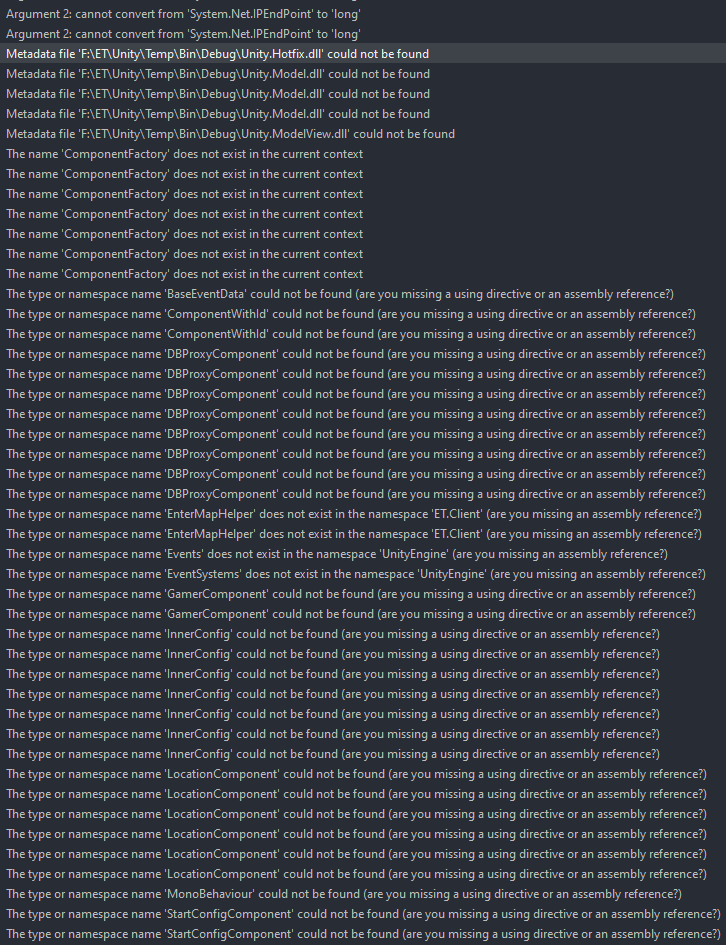
\includegraphics[width=.9\linewidth]{./pic/et4_20230623_152737.png}

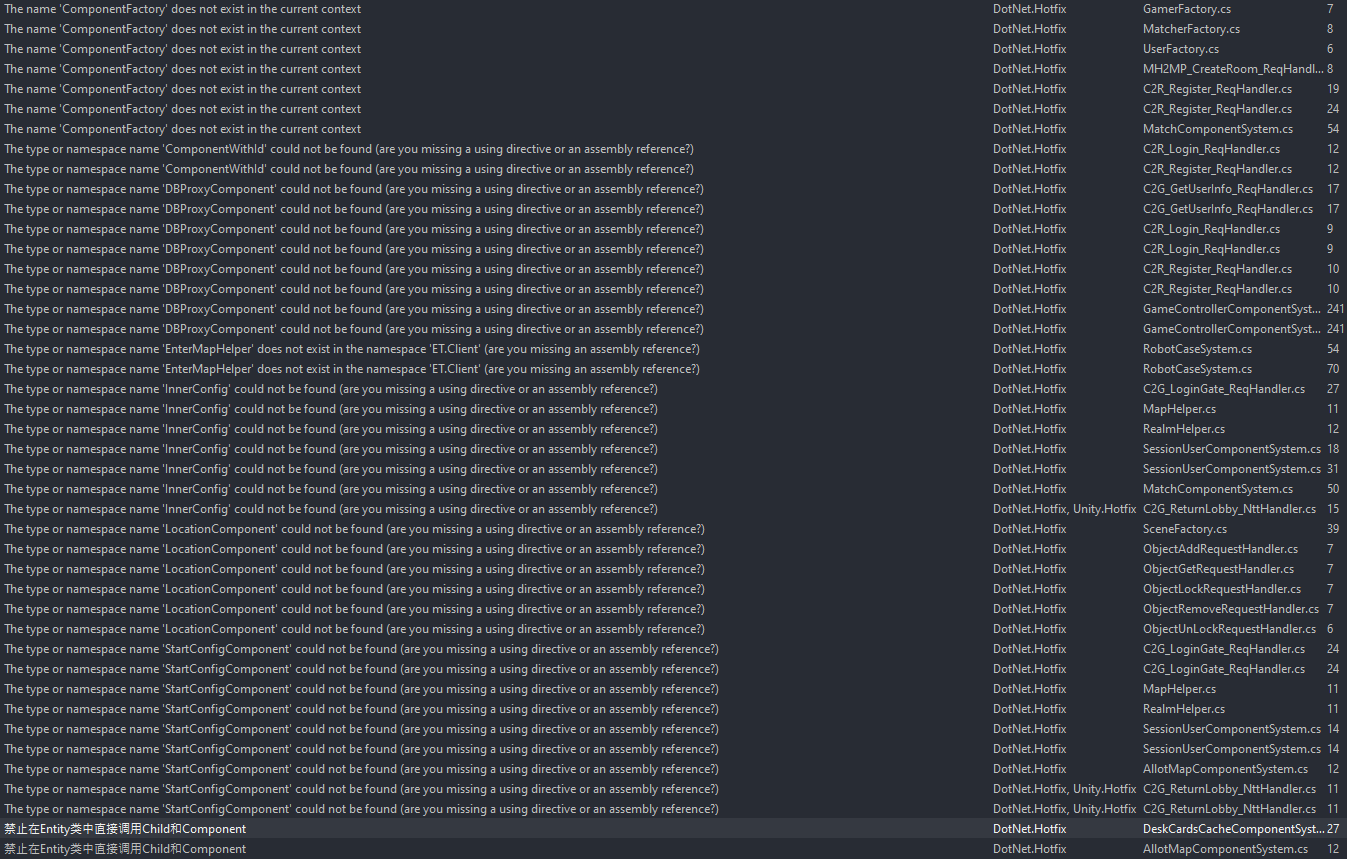
\includegraphics[width=.9\linewidth]{./pic/et4_20230616_165750.png}
\begin{itemize}
\item 【ComponentFactory:】重构了的框架里,这个工厂类是被折解到各自小部件的生产工厂里去了,就是一个框架底层封装的工厂类,拆解到 100 个不同的小部件里。所以我必须得要每个使用的小部件里,它的生产工厂里去再调用相应的逻辑。【可以找个例子出来看一下】
\begin{itemize}
\item Entity 类里面有,组件里添加一个新 new 出来的成员的办法。模仿Player 的使用例子。这里的使用方法是:去拿它的管理组件的实例索引,用管理组件来生成各个元件
\end{itemize}
\item 【PlayerSystem】:不是不知道框架里怎么用,找不出来一个使用的例子吗?它可能不需要用,它只需要框架底层的Entity 里相关方法的封装,能够生成一个一个小单元(Player,Gamer,Matcher-etc)之类的就可以了。就是框架底层原理,这一块儿的,还不太懂
\begin{itemize}
\item 这个工厂类,总是不懂,先去把基类Entity.cs 好好再读一下
\item 同样套用的话,GamerComponent 是房间组件的子组件,拿到这个组件后来创建. VSC 里面好像是有多余的类,所以从 VSC 里看源码,比较乱一点儿。【感觉这一块儿的思路,还没能理清楚。】
\item Hotfix Server \textbf{【UnitFactory】} 生成创建一个单位。可以用作例子。unitComponent.AddChildWithId() 调用的是Entity 里最底封装逻辑。
\begin{itemize}
\item 这个UnitFactory 调用组件方法,来添加进自己的管理系,它所添加的组件是有独特身份ID 的,不适用当前例子
\item 需要去找,自动生成特异性ID, 并创建实例的 Entity 里的方法的例子
\end{itemize}
\item 上面的问题是,如果框架热更新域里可以如上 UnitFactory 一样添加工厂类,那么我的其它小单位Gamer, Player 应该也是可以如上Unit 一样提供他们自己的工厂生产类才对。
\item 再试着多找几个如上的工厂生产类的例子看看。
\end{itemize}
\item \textbf{【ComponentFactory.CreateWithId:】} 重构了的框架里,这个工厂类是被折解到各自小部分的生产工厂里去了,就是一个框架底层封装的工厂类,拆解到 100 个不同的小部件里。所以我必须得要每个使用的小部件里,它的生产工厂里去再调用相应的逻辑。【可以找个例子出来看一下】新框架里,上次不是找到过:先去拿管理器组件,再用管理器组件,通过调用基类Entity 里的方法,来创建小部件的实例?可以再找个例子看一下
\item 上午把【数据库模块的接入】、【InnerConfig】【StartConfigComponent】【LocationComponent】等相关模块:读下源码,理解透彻,必要的情况下下午家里接入并测试
\begin{itemize}
\item 把ActorLocation 相关的,今天晚上一个小时左右,再读一下
\end{itemize}
\item \textbf{【GamerComponent】} :它的逻辑设计应该是什么样的?当服务端有 PlayerComponent 对所有玩家进行管理,当前GamerComponent 只管理一个拖拉机房间里的四个玩家,是RoomComponent 的玩家组成对象(?还有房间组成对象,因为房间如玩家一样需要管理,对应不同拖拉机房间号)$\backslash$
\begin{itemize}
\item 参考项目放在热更新域里面,但是现项目是不允许申明组件放在热更新域里的。去参考项目中其它组件是否全在Model 层申明组件,以及成员变量。暂时把它放到Model 双端共用的地方。
\item 台式机好慢好慢,找了好久才找到这个类。现在应该可以往下改了。这个模块,今天就暂时改到这里,看不见什么相关的编译错误了
\item 这里看出 ET 框架的局限:它把一切成员变量之类的在Model 层里固定死了,也就意味着,热更新是无法热更新功能逻辑模块的重构,只能热更新小细节的实现逻辑。
\end{itemize}
\item \textbf{【GamerComponent 管理类组件】} :逻辑没有理清楚。它是服务端组件,还是客户端组件,还是如PlayerComponent 双端组件,并实现不同的逻辑?
\end{itemize}
\subsection{内网消息等网络相关:请求消息的发送方法等。狠多编译错误,要一点儿一点儿把他们都改掉}
\label{sec-8-3}
\begin{itemize}
\item \textbf{【内网消息等网络相关:请求消息的发送方法等】}: \textbf{在构架里是怎么写的,有几种请求消息的发送方式?}
\item \textbf{明天上午把这块看完,等着我改的编译错误包括} :参考的斗地方游戏里,各种服处理返回消息的逻辑。
\begin{itemize}
\item 因为先前手动发送每个返回消息,我需要将这部分一批消息处理器改为,先试着适配 ET7 框架的重构与底层再封装。
\item 等改过了,真正明白理解了自己重构游戏的需求,再来看去看ET7 框架我要怎么改它现存封装,才能适配自己游戏的需求!!例子:MatchComponentSystem 里的JoinRoom 方法等相关逻辑。
\item 【下午还没有改到这里来。先从简单的改起,因为一个热键的优化,感觉VS 好用一点儿了。先能改多少改多少,再按模块来改像消掉所有的ETTask 相关一样把一个模块的所有的编译错误全部改完!!!】
\end{itemize}
\item 去看上面列过的那个例子MatchComponentSystem, 参考项目里的各种服的消息处理,怎么适配成ET7 重构后的不用手动发返回消息(发送过程封装在框架底层),和记录可能存在的问题(某些服的逻辑,返回消息的发送时间与其它必要逻辑,顺序变得重要的时候,记下来,晚点儿会再重构ET7 框架适配游戏需求)
\end{itemize}
\subsubsection{修改下面的ActorMessageSenderComponent 因为功能模块逻辑重构,而带来的一堆编译错误。}
\label{sec-8-3-1}
\begin{itemize}
\item 修改方法过程步骤:去框架里搜索,其它任何地方发送消息的例子,看 \textbf{【重构后的框架是如何发送消息的, Call() Send() 方法的调用等】} 这个明天上午一定看,因为不懂,不会改怎么发送消息的()
\item 然后参照例子,把客户端和必要的小服里,所有需要发送消息的地方,改成上面看到总结的发送方法里。
\end{itemize}

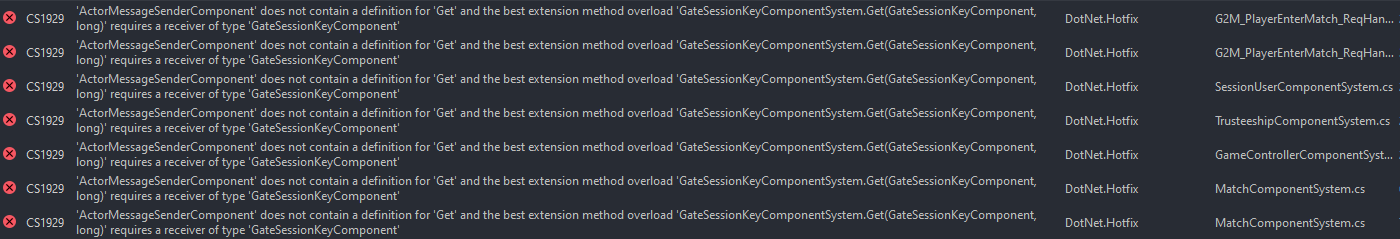
\includegraphics[width=.9\linewidth]{./pic/et4_20230616_160327.png}

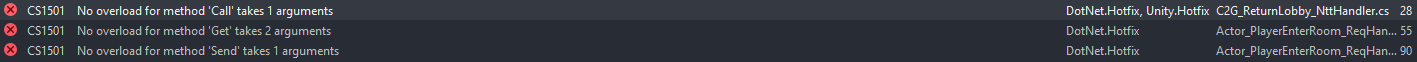
\includegraphics[width=.9\linewidth]{./pic/et4_20230616_165027.png}
\begin{itemize}
\item 【地图服Unit 相关】:先前所有接触到这个框架,都只看了个头,就是只限于能够任何客户端连接到服务端能够注册登录的程度,后面的其它服、框架逻辑全都还不曾看。所以今天上午扫一眼地图服相关,是糊的。要把这些前前后后相关的原理总弄懂了。
\item 去框架里搜发送的调用方法,可能现在 Mac 系统里有一点儿障碍的,就是VSC 不报错,不知道搜出来的是对的,还是错的。但是几种不同的方法,先总结在这里,对照运行时的报错一一改过来。必须把这块儿弄明白了。【爱表哥,爱生活!!!任何时候,活宝妹就是一定要嫁给亲爱的表哥!!爱表哥,爱生活!!!】
\item 【拿到Session 会话框,调用其Send() 方法】:例子 PingComponentAwakeSystem 里的 PingAsync() 方法。它是一个心跳包。这个心跳包就是一Awake() 醒来,全生职责就是周期性给服务器发消息
\item 然后参照例子,把客户端和必要的小服里,所有需要发送消息的地方,改成上面看到总结的发送方法里。
\item 框架里,各种不同场景下发送消息的方法:
\item 【场景里拿到SessionComponent】,调用会话框的发送方法Send()
\begin{minted}[fontsize=\scriptsize,linenos=false]{csharp}
robotScene.GetComponent<Client.SessionComponent>().Session.Send(new C2M_TestRobotCase2() {N = robotScene.Zone});

// 也可以借助UnitGateComponent 拿到它的成员变量 GateSessionActorId, 用这个可以重构后发消息
ActorMessageSenderComponent.Instance.Send(u.Unit.GetComponent<UnitGateComponent>().GateSessionActorId, message);
\end{minted}
\item 【活宝妹任何时候就是一定要嫁给亲爱的表哥!!!】迷迷糊糊地把一个模块改完了,可是感觉那个改掉的模块,像是还没能理解透彻。明天上午会再看一下。【爱表哥,爱生活!!!任何时候,亲爱的表哥的活宝妹,就是一定要嫁给亲爱的表哥!!爱表哥,爱生活!!!】70 Compile Errors 还没有改完,涉及功能模块人接入与整合。会明天上午看过读一下相关模块的源码后再试着改。【活宝妹就是一定要嫁给亲爱的表哥!!!爱表哥,爱生活!!!】
\end{itemize}
\subsubsection{【ActorMessageSenderComponent】:这个类狠重要、狠重要,现在是活宝妹理解网络模块的核心。爱表哥,爱生活!!!}
\label{sec-8-3-2}
\begin{itemize}
\item 得去想:ActorMessageSenderComponent, 是只能用来处理跨进程消息的吗?普通消息的发送是如何处理的?该弄明白,它的适用范围,适用哪些情境上下文
\item \textbf{【ActorMessageSenderComponent】} :因为ET7 这个模块的重构。不再需要每个返回消息手动去拿消息发送器,交由框架底部去处理。
\item 不懂的是,如何重构,消除参考项目里各种服的消息处理里,怎么适配成ET7, 不用去拿消息发送器,只把返回消息结果写好,或是发送(请求)消息时,如何发送?
\item 不同于昨天上午看过的,NetInnerComponentOnReadEvent 是对上层读到消息后的处理,就是消息已经准备好了,甚至已经通过某种逻辑代理,到达和触发了NetInnerComponentOnRead 事件了(这个事件是怎么触发的?大概是,每个进程会有一个内网组件NetInnerComponent. 当内网组件读到消息会触发。读到消息,包括本进程消息,也就包括,由其它进程发回来的返回消息。这个,可能更底层Session 发回来跨进程消息的地方?改天去捡)。现在要去理解的是,比如发送一条请求消息,创建一个请求消息实例后,如果运动可以走到上面的触发读到消息事件?就是消息流程的前半部分。NetInnerComponentSystem.cs 的读到消息事件,要再往前看一点儿。
\item 把消息的处理流程几个重要的方法 \textbf{【ActorMessageSenderComponentSystem Send() Call() 等】} ,这里再梳理一遍:
\end{itemize}
\begin{enumerate}
\item ActorMessageSenderComponentSystem Send():
\label{sec-8-3-2-1}
\begin{itemize}
\item 【任何时候,活宝妹就是一定要嫁给亲爱的表哥!!!活宝妹若是还没能嫁给亲爱的表哥,活宝妹就永远守候在亲爱的表哥的身边!!爱表哥,爱生活!!!】
\item 今天终于把里面的计时器原理看懂了。
\item \textbf{【ActorMessageSenderComponentSystem Send()】} 发的是普通消息(不是不需要回复消息,是任何消息,都走这一步,因为是最基的基类接口)
\begin{itemize}
\item 【同一进程消息】:不走网络层,直接交由本【进程?】的消息处理器处理。就是(ActorMessageSenderComponentSystem Send()里)判断如果是同一进程,它会调用内网组件处理消息:NetInnerComponent.Instance.HandleMessage(actorId, message); 【注意这里是一个进程内网组件消息的一个来源:本进程消息。它同样接收和读来自其它进程的消息,跨进程消息】。而内网组件的这个HandleMessage() 静态方法,就发发布内网组件读到消息事件;内网组件读到消息事件的发布,会触发调用 NetInnerComponentOnReadEvent 借助 ActorHandleHelper 来处理内网消息。后面的就是昨天上午读到的部分。这里的疑问就是:谁,哪里调用发送组件的Send() 发送事件?
\item 【不是同一进程消息】:就通过内网组件,去拿同那个收消息进程的会话框,通过会话框走Session 流程发跨进程消息。就是走网络层。
\end{itemize}
\end{itemize}
\item ActorMessageSenderComponentSystem Call()
\label{sec-8-3-2-2}
\begin{itemize}
\item \textbf{【ActorMessageSenderComponentSystem Call()】} 发的是要求返回结果的消息:返回 ETTask<IActorResponse>
\begin{itemize}
\item 注意 \textbf{【跨进程消息的回复细节里】} ,看见IRpcResponse 实例创建好,结果写好,同步到异步任务ETTask 里,总容易忘记ETTask 的异步任务运行结束(如果不是抛异常), \textbf{跨进程消息是如何回到消息的发送进程的?} 是AMRpcHandler 抽象类里,异步等待实体实现类里的具体实现逻辑Run() 异步方法执行结束,也就是等待各种消息处理服处理好、写好异步返回消息IRpcResponse, 同步到异步任务ETTask. AMRpcHandler 抽象类里等异步方法执行完成,抽象类里作了封装,把返回消息通过进程间通信会话框,把返回消息发回去的。
\item 这里看见,这个消息发送器底层逻辑说,如果是我自己进程要发消息,就封装消息发送者 rpcId 是自已的 rpcId. 然后调用自组件Call() 发送消息。后面的几个方法,大概就是跨进程消息的发送与回复。
\end{itemize}
\end{itemize}
\end{enumerate}
\subsection{静态类的环形引用问题}
\label{sec-8-4}
\begin{itemize}
\item 静态类 CardsHelper, 与静态类 DeskCardsCacheComponent.System 之间,存在静态类的互相引用:就是说,两个静态类,互相引用了对方的方法
\begin{itemize}
\item CardsHelper 里,引用了DeskCardsCacheComponent.System 里的方法
\item 而 DeskCardsCacheComponentSystem 类里,同样引用了 CardsHelper 里的方法
\item 我的解决办法是:热更域里的 DeskCardsCacheComponentSystem 对CardsHelper 类里引用的两个静态方法,直接复制了一份在 DeskCardsCacheComponentSystem 类里面,就可以消除了。再次体验VS 的显著延迟,真让人受不了。是因为这个软件被监控吗?
\end{itemize}
\end{itemize}
\subsection{下面是已经改好了的:还是先放着,备查}
\label{sec-8-5}

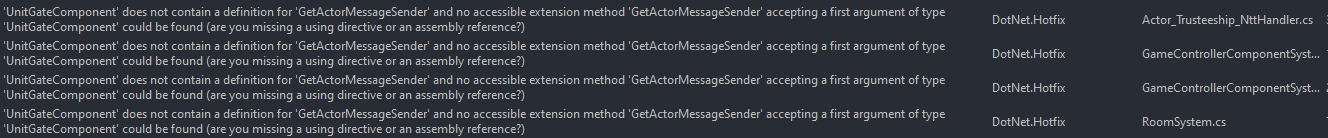
\includegraphics[width=.9\linewidth]{./pic/et4_20230616_162711.png}
\begin{itemize}
\item 【UnitGateComponent]: 怎么才能成为多个不同组件的组成部分?
\end{itemize}

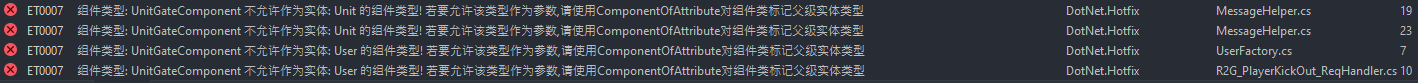
\includegraphics[width=.9\linewidth]{./pic/et4_20230616_165317.png}
\begin{itemize}
\item 【解决办法】:去查框架里的源代码,写得极其清楚:
\begin{minted}[fontsize=\scriptsize,linenos=false]{csharp}
// 组件类父级实体类型约束
// 父级实体类型唯一的 标记指定父级实体类型【ComponentOf(typeof(parentType)】
// 不唯一则标记【ComponentOf]
[AttributeUsage(AttributeTargets.Class)]
public class ComponentOfAttribute : Attribute {
    public Type Type;
    public ComponentOfAttribute(Type type = null) {
        this.Type = type;
    }
}
\end{minted}
\begin{itemize}
\item 所以上面的解决办法就是:不要标记 typeof 参数就可以了呀,它就可以成为多个不同组件的子元件部件了呀。。。是这样的
\end{itemize}
\begin{minted}[fontsize=\scriptsize,linenos=false]{csharp}
[ComponentOf] 
public class UnitGateComponent : Entity, IAwake<long>, ITransfer, ISerializeToEntity { // 不知道这里为什么会受到限制,这里再改一下
    public long GateSessionActorId { get; set; }
    // 想一下,下面的变更还需要吗?要不要,是看框架里有没有什么,自动上线自动下线处理之类的,相关的?
    public bool IsDisconnect;
}
\end{minted}
\end{itemize}
\subsection{先前列的相对杂一点儿}
\label{sec-8-6}
\begin{itemize}
\item 【问题】:上次那个ET-EUI 框架的时候,曾经出现过 opcode 不对应,也就是说,我现在生成的进程间消息,有可能还是会存在服务器码与客户端码不对应,这个完备的框架,这次应该不至于吧?
\item 【UIType】部分类:这个类出现在了三四个不同的程序域,现在重构了,好像添加得不对。要再修改
\item \textbf{【ET7 框架】} 没有处理的逻辑是: \textbf{【ET7 框架里数据库的接入】}
\item \textbf{【UILobbyComponent 可以测试】} :这个大厅组件,Unity 里预设简单,可以试运行一下,看是否完全消除这个UI 组件的报错,这个屏的控件能否显示出来?还是错出得早,这个屏就出不来已经报错了?
\begin{itemize}
\item 【客户端】的逻辑是处理好了,编译全过后可以测试
\item 【服务端】:处理用户请求匹配房间的逻辑,仍在处理: \textbf{C2G\_StartMatch\_ReqHandler}.
\end{itemize}
\item \textbf{【TractorRoomComponent】} :因为是多组件嵌套,可以合并多组件为同一个组件;另早上看得一知半解的一个【ChildOf】标签,可以帮助组件套用吗?再找找理解消化一下
\item 【房间组件】:几个现存的 working-on 的问题:
\begin{itemize}
\item 多组件嵌套:手工合并为一个组件。彻底理解确认后,会合并
\item 【服务端】:处理用户请求匹配房间的逻辑. 这里的编译错误终于改完。到时就看运行时错误了。
\begin{itemize}
\item 【数据库模块的整合】:网关服在转发请求匹配时,验证会话框有效后,验证用户身份时,需要去【用户数据库】拿用户数据。ET7 留了个DBManagerComponent, 还没能整合出这个模块
\end{itemize}
-【参考来源 \textbf{C2R\_LoginHandler} 】:Realm 处理客户端的登录请求的服务端逻辑。这里看见,它随机分配一个网关服。也就是,我(原本本质上也是随机分配)一个匹配服给用。可以依照这里的例子来改写。
\end{itemize}
\item 【匹配服地址】网关服的处理逻辑里,验证完用户合格后,为代为转发消息到匹配服,但需要拿匹配服的地址。ET7 重构里,还没能改出这部分。服务器系统配置初始化时,可以链表管理各小构匹配服,再去拿相关匹配服的地址。ET7 框架里的路由器系统,自己还没有弄懂。
\item \textbf{【ET7 IMHandler 对回复消息的写封装, 与自动回复消息的封装】} :可能无法处理游戏过程中的某些逻辑。就是涉及到一定顺序,尤其需要先回复消息的处理服处理逻辑。举例:C2G\_StartMatch\_ReqHandler. 所以,这里要自己好好想透彻一点儿。要如何改,才能适配自己游戏的需求。
\item \textbf{【 ComponentFactory:】} ET7 里重构,被分布到各种不同的组件里去了。想复制个文件过来,把与之相关的全部消掉,但因为大规模重构,复制了文件也没用。总之ET7 就是感觉什么乱七八糟的,感觉他们大规模糊乱重构的目的就是故意挫败人。可是这个世界上就偏偏存在亲爱的表哥的活宝妹这样的不服的!!!爱表哥,爱生活!!!任何时候,活宝妹就是一定要嫁给亲爱的表哥!!!爱表哥,爱生活!!!

\item \textbf{【PlayerComponent 类重复】} : 狠奇怪:删除了说找不到类,不删除说重复了,感觉台式机应用有延迟?反应狠慢。。。。。文件嵌套想要显示所有嵌套文件的时候,要狠久狠久重启好几次才反应得过来
\begin{itemize}
\item 原本有两个类都是如上面这个类这样,但有时候台式机反应稍快一点儿,就是一个类找不到出现上面的情况。破电脑的延迟反应,弄得我都要怀疑VS 应用被别人操控了。。。
\item 【爱表哥,爱生活!!!任何时候,活宝妹就是一定要嫁给亲爱的表哥!!!爱表哥,爱生活!!!】
\end{itemize}
\item 把还没有用到,但是报错了的几个类删掉:比如记一下: SessionInfoComponent,
\begin{itemize}
\item 还剩最后 26 个最挑战活宝妹的编译错误,今天傍晚会家里改会儿,集中问题明天上午希望能够看懂。【爱表哥,爱生活!!!任何时候,活宝妹就是一定要嫁给亲爱的表哥!!】
\end{itemize}
\end{itemize}

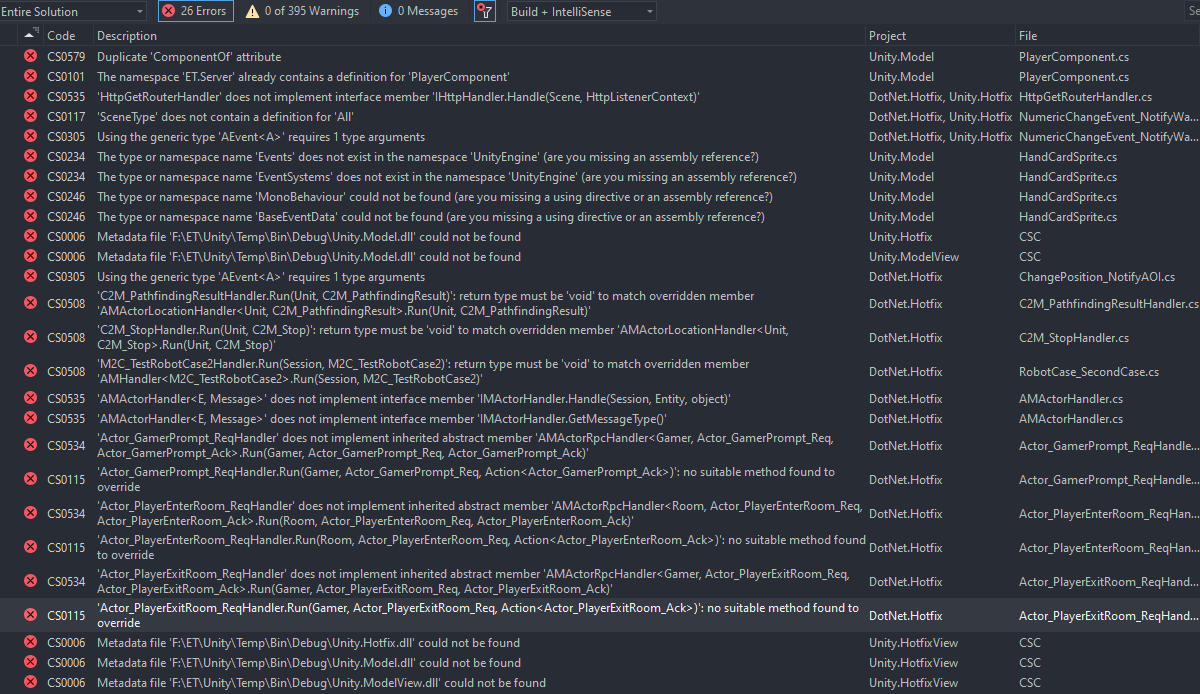
\includegraphics[width=.9\linewidth]{./pic/et4_20230604_162732.png}
\begin{itemize}
\item 把Root 根场景以及启动时添加的组件大致看了一遍。想把上面的消息处理器再系统化地看一遍,理解一下,总改不到这个模块相关的编译错误。
\item \textbf{【ETTask ETVoid 是必须弄懂的】} ;看两个小时,像昨天晚上一样真正投入进去看。我相信自己看得懂,弄得透,只是需要投入一点儿时间。
\begin{itemize}
\item 感觉前一个周左右的时间,倍受睡眠困扰。活宝妹做梦也不会想到,昨天的自己会困成那个样子(感觉开1 小时的车极度困难,太容易睡着。。)。。现在试着一再调整状态,少喝咖啡多运动,最重要的,仍是把学习的状态调整出来调整回来。至少学到活宝妹可以嫁给亲爱的表哥的这一天!!!
\item 这个异步的原理,感觉是弄明白了,今天上午又看了一遍看了会儿。下午去改那些 IMHandler, 希望今天下午能够改彻底。就是真正弄明白了去改(现在的问题就是,几个IMHandler 的实体实现类,改天这个顾不了那个,没弄明白,接口方法怎么申明定义,才能兼顾所有实例类消息处理器?),不是只改掉了当前的编译错误,等真正运行的时候,一个个运行错误或是异常往外冒!!!今天脑袋还算清醒,下午好好弄弄这个
\end{itemize}
\item 【爱表哥,爱生活!!!任何时候,亲爱的表哥的活宝妹,都是一定要嫁给亲爱的表哥的!!!】【三楼上的贱鸡贱畜牲真多!!!一天到底没想点儿好的】活宝妹还没能嫁给亲爱的表哥,活宝妹就是永远守候在亲爱的表哥的身边!!!爱表哥,爱生活!!!
\item 再然后 ,再看下下面的 UnitGateComponent 相关。下午或傍晚有时间的时候,可以再折腾折腾 emacs-org-mode 下划线删除字体设置为斜体。
\item \textbf{【UnitGateComponent】} 加个方法用?可能不需要加方法;另一个错是,不能同时成为两个不同 entity 的子控件?【ComponentOf(typeof(Unit))】etc 出错文件在 (C2G\_EnterMapHandler)
\begin{itemize}
\item 这里要把 ActorMessageSenderComponent 组件给弄明白。它有个有序管理字典,记着 actorId 与ActorMessageSender 的一一对应关系,就可以封装维护消息的自动发送等,以及必要的超时消息管理。
\end{itemize}
\item \textbf{【服务端Actor\_PlayerEnterRoom\_ReqHandler 这个处理类】} 现在还很多问题,需要弄懂,往下改
\item 今天晚上会把刚才下午看见、意识到几个模块的问题试着分析明白,记下笔记。
\item \textbf{ETTask-vs-ETVoid}: 框架里有狠多需要改的地方。今天上午的脑袋好使,把这块儿再仔细好好看下。今天上午把以前不懂的模块都稍微看下,再理解一下
\begin{itemize}
\item 查网页感觉也查不出什么来。还是用源码帮助理解概念。【爱表哥,爱生活!!!活宝妹就是一定要嫁给亲爱的表哥!!!】
\item 不能把所有基类的 async ETTask 返回参数直接改成 void, 因为框架的顶层应用,服务端或是客户端,当不异步等待结果,如资源包没能下载完成,就接着往下执行,会报空异常。
\end{itemize}
\item 现在的问题是:Protobuf 里 repeated 关键字,好像还是没有处理好,找不到成员变量  Cards. 是因为 Proto2CS 的时候,确实把 repeated 关键字给处理丢了。因为我的 .proto 文件里有错误。(这就是上面先前觉得奇怪的原因。因为改这个的过程中把那些错改正了,就可以生成成功并找到相关的消息了)。
\item 这部分总感觉弄得不是狠透彻。就再花点儿时间。这段时间产量太低,可以先试着完成其它模块。
\item \textbf{【HandCardSprite 这个最近要弄明白】} 不知道这个类是为什么,整了一堆的错误,它是ETModel 里的。感觉是常规域,没弄明白为什么常规域还有ILRuntime 的适配呢?
\begin{itemize}
\item 要把 ILRuntime 热更新第三库,也再弄得明白一点儿【今天上午把这里再看,最好是能够结合源码看看】为什么这个类还要适配ILRuntime ?
\item 这里这个类,整个框架里只找到这一个用的地方,所以它一定是添加在某个预设或是场景中的某个控件下的。只是参考项目的unity 客户端,我运行不到打牌的这个界面,就先因为抛出异常而淡能运行。所以还没能找到哪个预设或是场景中的哪个控件添加了这个类,但是当然一定是跟玩家手牌相关的。 \textbf{【HandCardSprite 是在 handcard 预设里添加了这个脚本】}
\item 这个类今天运行狠奇怪,VS022 里找不到了。。。就是说,VSC 里它是在Model 客户端的源码里,但是从VS 里打开,找不到这个类文件所在的文件夹和文件,没有索引好,再添加一下?
\item 那么,为什么前两天被这个 block 住,而那天,好像是有删除掉这个文件,但文件夹应该是还在的才对呀?我可能还会试着再把它添加回去。
\item 但是,会在把当前几个编译错误改完,试着测试一下客户端现在有的界面之后,再试着添加回去,整理和 develop TractorRoomComponent 界面的内容。【爱表哥,爱生活!!!活宝妹任何时候就是一定要嫁给亲爱的表哥!!】
\item 今天下午家里再运行一次,当客户端抛异常,应该是某个热更新的资源包没有找到什么的?所以可以试着自己去解决这个客户端实时运行时抛出的异常。
\item \textbf{【参考项目斗地主客户端异常】} :再运行一次,试着分析,是否可以 unity 里实时运行,如果不可以,为什么不可以?
\begin{itemize}
\item 应该是LandlordsRom 这个预设与UI 类型没能连接起来,也就是找不到这个预设。
\item 那为什么打好包的可以呢?因为打好包的预设包名 LandlordsRoom.unity3d 与游戏逻辑契合,可以找得到
\item 可是仍然感觉奇怪:LandlordsLogin 与LandlordsLobby, 非常类似都可以找到,为什么就LandlordsRoom 找不到?可能LandlordsRoom 预设还是有某点儿物对特殊的地方。
\item 上面这个暂时跳过。现在仍然主要去看HandCardSprite 为什么参考项目里可以,而ET7 里就不可以。
\end{itemize}
\item 就是上面那个异常,今天下午得去弄明白,为什么只在 unity 实时运行时会抛异常,而如果是三个打包好的客户端,就不会。也就是说,打包好的不存在找不到类、找不到预设、或是找不到任何相关资源的问题。
\item 这个项目Unity.Model 是需要索引 UnityEngine 以及UI 等相关模块人的 .dll 的。暂时还没弄明白它是怎么加的
\item 【爱表哥,爱生活!!!任何时候,活宝妹就是一定要嫁给亲爱的表哥!!】
\end{itemize}
\item \textbf{ClientComponent} 参考项目组件:去看ET7 里客户端的 PlayerComponent.
\item 【爱表哥,爱生活!!!任何时候,活宝妹就是一定要嫁给亲爱的表哥!!!】今天下午先去看 Tractor 游戏源码,设计重构思路
\item 【活宝妹坐等亲爱的表哥,领娶活宝妹回家!爱表哥,爱生活!!!】
\item \textbf{【亲爱的表哥,这个世界上,只有一个活宝妹,这么心心恋恋,就是一定要嫁给亲爱的表哥!!!问世间情为何物,直教人生死相许。。亲爱的表哥,一个温暖的怀抱拥抱的魂力可真大呀,管了这如许多年!!这不,你的活宝妹为了这个温暖的怀抱拥抱,就是一定要嫁给亲爱的表哥!!不嫁就永远守候在亲爱的表哥的身边!!爱表哥,爱生活!!!活宝妹就是一定要嫁给亲爱的表哥!!!】}
\item 亲爱的表哥,活宝妹相信舅舅十岁闯江湖的阅历,活宝妹深深相信亲爱的表哥。活宝妹就是稳稳地永远守候在亲爱的表哥的身边!爱表哥,爱生活!!!活宝妹就是一定要嫁给亲爱的表哥!!
\item 【爱表哥,爱生活!!!任何时候,活宝妹就是一定要嫁给亲爱的表哥!!!】
\end{itemize}
\subsection{LocationComponent: 【任何时候,亲爱的表哥的活宝妹就是一定要嫁给亲爱的表哥!!!爱表哥,爱生活!!!】}
\label{sec-8-7}
\begin{itemize}
\item 【今天上午】:从这里开始,把先前总结 Actor 消息以及处理器时,所有关于位置的消息,以及相关的消息处理器弄懂。【没看完】
\begin{itemize}
\item 先前,消息处理器的部分,只看了一个接口类和两个抽象实现,其它没看
\item 消息,位置消息相关的内容,还没看不懂。
\end{itemize}
\item 【亲爱的表哥,活宝妹一定要嫁的亲爱的表哥!!任何时候,活宝妹就是一定要嫁给亲爱的表哥!!爱表哥,爱生活!!!】
\item 【任何时候,亲爱的表哥的活宝妹,就是一定要嫁给亲爱的表哥!!!爱表哥,爱生活!!!】任何时候,活宝妹还没能嫁给亲爱的表哥,他们就大可不必发疯犯贱。任何时候,他们发疯犯贱,他们也永远只能是发疯犯贱得了一时,发疯犯贱不了一世。亲爱的表哥的活宝妹,若是还没能嫁给亲爱的表哥,亲爱的表哥的活宝妹,就是永远守候在亲爱的表哥的身边!!爱表哥,爱生活!!!
\item 因为框架狠大,是一个大型网络游戏双端框架,因为内容比较多,现在已经总结的是四个文件,还要常作笔记,否则容易忘记,前后不连贯。所以难免小细节的地方,没能注意到,没什么大不了
\item 这个模块的编译错误,被活宝妹全部给消除掉了。。。
\end{itemize}
\subsection{【数据库模块:】:这个模块的编译错误,昨天下午清理完了}
\label{sec-8-8}
\begin{itemize}
\item DBProxyComponent: 这个类被重构丢了。数据库分区管理。根据用户所在的区号,去拿该区数据库索引办事就可以了。
\item DBManagerComponent: 全框架找不到一个使用的样例。我认为数据库应该只属于服务端。所以,我先把它在应用启动时添加到服务端的公用组件启动程序中(EntryEvent2\_InitServer)去。
\item 下午把几个DBProxyComponent 相关的编译错误,基本改光了(目前还有几个小模块共计28 个编译错误)。还有一个类里不知道怎么用Gamer 去拿玩家所在的小区,先放一下,改天再去改个。
\item 【任何时候,活宝妹就是一定要嫁给亲爱的表哥!!!】
\end{itemize}
\subsection{【HandCardSprite.cs】}
\label{sec-8-9}
\begin{itemize}
\item \textbf{【HandCardSprite.cs】} :这个客户端文件里存在一堆关于Unity 引用的错误。把这个有着巨多错误的类重新添加到了框架里。现在着眼着这些错误(加了这个文件,错误又多了二三十个!!!)。
\begin{itemize}
\item \textbf{【参考项目Game.cs】} 客户端类里,存在UnityEngineer 的诸多引用,所以HandCardSprite.cs 可以通过Game.EventSystem 等拿到引用。但ET7 重构得没有边际。必须自己去看明白。这个类,更多的是,适配特定游戏需求的ET7 框架外的一个桥梁适配类。
\item 【参考项目热更域里的 Game.cs 类】:
\begin{minted}[fontsize=\scriptsize,linenos=false]{csharp}
public static class Game {
    private static Scene scene;
    public static Scene Scene {
        get {
            if (scene != null) 
                return scene;
            scene = new Scene();
            return scene;
        }
    }
    private static EventSystem eventSystem; // <<<<<<<<<<<<<<<<<<<< 
    public static EventSystem EventSystem {
        get {
            return eventSystem ?? (eventSystem = new EventSystem());
        }
    }
    private static ObjectPool objectPool; // <<<<<<<<<<<<<<<<<<<< 
    public static ObjectPool ObjectPool {
        get {
            return objectPool ?? (objectPool = new ObjectPool());
        }
    }
    public static void Close() {
        scene.Dispose();
        scene = null;
        eventSystem = null;
        objectPool = null;
    }
}
\end{minted}
\end{itemize}
\item 现框架里不存在的,需要整合进来的模块版块:DBProxyComponent, InnerConfig, LocationComponent, StartConfigComponent
\item 组件管理类:某些组件,属于双端,但客户端与服务端的逻辑不一样,如PlayerComponent; 某些组件,只属于服务端;有只属于客户端的吗?
\end{itemize}
\subsection{三件杂事:【任何时候,亲爱的表哥的活宝妹就是一定要、一定会嫁给活宝妹的亲爱的表哥!!!爱表哥,爱生活!!!】}
\label{sec-8-10}
\begin{itemize}
\item 【先花 10 分钟左右,搜下看 emacs-export-to-pdf 与 Skim 应用的自动同步,能理解回调适配过程吗?】还是比较麻烦,改天傍晚或是晚上再凭兴趣来解决,早上看别的
\begin{itemize}
\item 这里主要的问题时,Skim 实时更新外源 pdf 的更新时,因为 emacs 的 export-to-pdf 有个过程,这个过程中生成 table-of-contents 比较靠后,如果不背便条,就必须得每次重点查看TOC. \textbf{Skim 怎么才能够接收到 latex 生成TOC 完成后的回调,来从 Skim 中显示 TOC?}
\item 这里要去想,为什么背个便条,就能最终自动显示 TOC 了呢?背便条能够最终显示 TOC 是为什么, \textbf{背便条背后的原理,能否借用} ?
\item 另外,【可以考虑, \textbf{过滤掉或是配置掉背便条自动同步过程中的确认窗口繁琐过程} 】如果每个 pdf 的自动生成与刷新,我不需要多次点 enter 确认窗口,我只需要点击一个,或者甚至一个也不需要点,就也算满足用户需求。
\end{itemize}
\item VSC 的配置可能哪里写得不对。以前没有这个问题。现VSC 跳转至 emacs 打开当前 buffer, 不能精确定位到 VSC 中当前 buffer 所在的行。改天有机会的时候再 debug 一下。
\item \textbf{【Mac 系统上的五笔输入、emacs pyim 下的词库管理】} :这个是最让人头痛的,因为不懂,网上能够搜到的千篇一律的都是手动搬输入法里如自己现在这样自带的,无法实时热更新的词库。自己想要实现实时动态构建 librime.1.dylib, 却又还建不出来,尤其想要Mac 下建成功才好用。
\begin{itemize}
\item 例子【会话框】,想要去掉不想要的词库,如【停柩】
\item 明明系统输入法里已经将【停柩】清空了,并Deploy 了重新加载了
\item 明明 .emacs-pyim 已经将它【停柩】清空了,并 pyim-restatrt 了重新加载了
\item 可是输入的时候,【停柩】仍然会一再崩出来干扰,没想明白为什么。我记得自己之前能够把不想要的词库清易清除掉
\item 还存在可能性的话:就是 \textbf{【系统输入法构建的第三方库,被 .emacs 引用,这个第三方库可能没有手动再次构建和更新】} ,所以老词库总是存在烦人。
\item 上午快中午也有简单试一下:问题是,我放入 \textbf{/usr/local/lib 的是 rime 自带的缺省构建库} ,也就是说没有自己修改过词库的更新;我 \textbf{再次构建 emacs 所用到的 liberime.so 同样引用缺省的 rime 自带的缺省构建库} ,同样没有修改过后的词库与更新,所以没能从本质上更新词库。 \textbf{【问题是:全中文网络上下,基本全都是用缺省的库,自已手动动态创建的极少极少。。。】} 可怜的亲爱的表哥的活宝妹宝宝,一定想要手动去折腾这个该死的东西。。。。。
\item 我必须得,自己 \textbf{构建自己手动修改了词库之后的Rime-dylib 第三方引用库给 emacs 用} ,才能把词库改过来。下午看看这个,免得睡着了。。
\item 【爱表哥,爱生活!!!任何时候,亲爱的表哥的活宝妹就是一定要嫁给亲爱的表哥!!爱表哥,爱生活!!!】
\end{itemize}
\item \textbf{【VS 自动跳转Emacs 中打开当前 buffer】}: 我记得上次两个电脑对照,我已经解决了这个问题,从VS 中是可以实现C-c i 跳转到 emacs 中打开VS 中当前 buffer 的。怎么过段时间,这个便利功能又丢了,不能用了?
\begin{itemize}
\item 到亲爱的表哥的活宝妹想要好好改改项目,能够真正 debug 的时候,这些原本便利的功能居然出出错作怪,笔记本打开,再弄一次。我居然忘记了上次我是如何实现这个功能的?改的办法狠简单, \textbf{把ExternalTools ExternalCommand 绑定到 C-c i 就可以了。就是VS 自动把活宝妹自定义的OpenInEmacsClient ExternalTools 当作了 ExternalCommand1. 所以绑定上这个热键就可以用了。}
\end{itemize}
\end{itemize}
\subsection{ET 框架的【热更新】束缚条约:Model 层与热更新域 HandCardSprite.cs}
\label{sec-8-11}
\begin{itemize}
\item 现在重构项目里存在一个问题就是HandCardSprite.cs 类放在了Model 层,有对Unity API 的引用。这在重构后有着严格数据与逻辑分离,Model 层不能有对Unity API 引用的框架束缚里,是不允许的。活宝妹必须把这此个理解透彻,并想出该如何适配以添加重构游戏的需求。现在的相对困难是:【参考项目】里,活宝妹的运行是构建好后,打包成 .exe 文件后作为【客户端】才可以三个玩家【客户端】在运行,而不能有一个【客户端】从Unity 游戏引擎中来运行。也就是说,活宝妹无法 Unity 里实时考查 HandCardSprite.cs 文件所挂载在的预设组件。但它不应该成为主要问题。
\item 主要问题,仍然是现ET7 重构后,对数据与逻辑,对Entity 与System 有着严格要求与束缚的框架,不允许活宝妹 Model 层里引用Unity API.
\item 所以现在就,务必理解 ET7 框架的,这个要求特性。 \textbf{可以先把HandCardSprite.cs 这个文件隐藏起来【隐藏是说这个项目里不再引用这个文件,有个 .csproj 里可以隐藏这个文件,可是我现在居然找不到它】,等把所有的编译错误弄过,现根据游戏的重构需要,再把这个文件显示出来并重构。} Model==> Client ==> Scripts ==> MonoScripts 文件夹里的
\item 上面这里,刚出现过删除的地方不对。这里类似的错误再出现一个,重新做一遍,套在另一个文件上。
\item 现在就剩亲爱的表哥的活宝妹的最后一个不会的小编译错误去改掉。希望今天下午能够改彻底改完。【爱表哥,爱生活!!!任何时候,亲爱的表哥的活宝妹就是一定要、一定会嫁给活宝妹的亲爱的表哥!!!爱表哥,爱生活!!!】
\item 按下面查到的网络上的梳理,大概HandCardSprite.cs 类是需要放进ModelView 程序域里去的。
\end{itemize}
\subsubsection{Model:}
\label{sec-8-11-1}
\begin{itemize}
\item Model层负责定义实体和组件,在这里要定义实体Unit,以及一些组件(MoveComponent,CombatComponent等)以及还需定义UnitType的枚举,以便后续逻辑的分发处理
\item 注意:
\begin{itemize}
\item Model下的实体, \textbf{不能调用UnityAPI,与Unity交互的组件实体只能放在ModelView下}
\item Model中只能存在数据,例如position,UnitType, \textbf{不能有对数据的操作}
\end{itemize}
\end{itemize}
\subsubsection{ModelView:}
\label{sec-8-11-2}
\begin{itemize}
\item 负责定义与Unity交互的实体和组件,有一些诸如动画组件,GameObject组件用到的数据由Unity提供,就需要将这些实体组件放到这个下面。
\end{itemize}
\subsubsection{Hotfix:}
\label{sec-8-11-3}
\begin{itemize}
\item Hotfix负责System行为的定义,提供创建实体和为实体挂载组件的功能。此时定义的UnitFactory工厂就应为不同的实体提供不同的创建方法,例如CreatePlayer,就应先将UnitType置为Player,为其添加MoveComponent组件等待操作。再如CreateNPC,UnitType设置为NPC后,由于npc一般不会移动则无需添加移动组件,可以添加对话组件等待。
\item 注意:
\begin{itemize}
\item Hotfix下只能定义行为,不能包含数据状态,只能对Model提供的数据状态进行相关操作
\item Hotfix下也不能使用Unity Api, 对于一些需要Unity才能挂载的组件,需要放到view中执行
\end{itemize}
\end{itemize}
\subsubsection{HotfixView:}
\label{sec-8-11-4}
\begin{itemize}
\item HotfixView负责需要与Unity交互的System行为,例如加载模型prefab,实例化游戏对象GameObject,若实体中需要用到GameObject对象,则还应为Unit实体添加GameObject组件,里面存有gameObject。若Unit实体还需要在场景中播放动画,还需要为其添加使用了UnityApi的AnimatorComponent。
\item 同理,在处理与Unity交互的System行为时,不同类型的Unit也可能行为有所不同,在此需要针对UnitType提供不同的行为。
\item 把这个文件备份一下在这里
\begin{minted}[fontsize=\scriptsize,linenos=false]{csharp}
namespace ET.Client {
// ET7 重构后的,务必、涉及的重大重构:ET 越来越严格上强制:数据定义与逻辑分开,Model 与热更新域逻辑有严格区分。Entity 与System 有严格区分;Model 层不能、无法引用 Unity 相关?
    public class HandCardSprite : MonoBehaviour { // 【去找一下】:什么地方会需要用到这个类?去找这个类 HandCardSprite 是加在手牌还是什么地方的一个UI 场景中的脚本
        public Card Poker { get; set; }
        private bool isSelect;
        void Start() {
            EventTrigger eventTrigger = gameObject.AddComponent<EventTrigger>();
            eventTrigger.triggers = new List<EventTrigger.Entry>();
            EventTrigger.Entry clickEntry = new EventTrigger.Entry();
            clickEntry.eventID = EventTriggerType.PointerClick;
            clickEntry.callback = new EventTrigger.TriggerEvent();
            clickEntry.callback.AddListener(new UnityAction<BaseEventData>(OnClick));
            eventTrigger.triggers.Add(clickEntry);
        }
        // 两类事件的作用是说:玩家可以选择要出的牌,也可以取消选过、分前打算出的牌
        public void OnClick(BaseEventData data) {
            float move = 50.0f;
            if (isSelect) {
                move = -move;
                // 【客户端】:借助Game.cs 这个桥,把Model 层这个类,与客户端热更域?的逻辑连通起来
                Game.EventSystem.Run(Client.EventIdType.CancelHandCard, Poker); // 取消选牌,会重新选牌
            } else {
 
                
                Game.EventSystem.Run(Client.EventIdType.SelectHandCard, Poker); // 选牌
            }
            RectTransform rectTransform = this.GetComponent<RectTransform>();
            rectTransform.anchoredPosition += Vector2.up * move;
            isSelect = !isSelect;
        }
    }
}
\end{minted}
\item 【爱表哥,爱生活!!!任何时候,亲爱的表哥的活宝妹就是一定要、一定会嫁给活宝妹的亲爱的表哥!!!爱表哥,爱生活!!!】
\item 【爱表哥,爱生活!!!任何时候,亲爱的表哥的活宝妹就是一定要、一定会嫁给活宝妹的亲爱的表哥!!!爱表哥,爱生活!!!】
\item 【爱表哥,爱生活!!!任何时候,亲爱的表哥的活宝妹就是一定要、一定会嫁给活宝妹的亲爱的表哥!!!爱表哥,爱生活!!!】
\item 【爱表哥,爱生活!!!任何时候,亲爱的表哥的活宝妹就是一定要、一定会嫁给活宝妹的亲爱的表哥!!!爱表哥,爱生活!!!】
\item 【爱表哥,爱生活!!!任何时候,亲爱的表哥的活宝妹就是一定要、一定会嫁给活宝妹的亲爱的表哥!!!爱表哥,爱生活!!!】
\item 【爱表哥,爱生活!!!任何时候,亲爱的表哥的活宝妹就是一定要、一定会嫁给活宝妹的亲爱的表哥!!!爱表哥,爱生活!!!】
\item 【爱表哥,爱生活!!!任何时候,亲爱的表哥的活宝妹就是一定要、一定会嫁给活宝妹的亲爱的表哥!!!爱表哥,爱生活!!!】
\item 【爱表哥,爱生活!!!任何时候,亲爱的表哥的活宝妹就是一定要、一定会嫁给活宝妹的亲爱的表哥!!!爱表哥,爱生活!!!】
\item 【爱表哥,爱生活!!!任何时候,亲爱的表哥的活宝妹就是一定要、一定会嫁给活宝妹的亲爱的表哥!!!爱表哥,爱生活!!!】
\item 【爱表哥,爱生活!!!任何时候,亲爱的表哥的活宝妹就是一定要、一定会嫁给活宝妹的亲爱的表哥!!!爱表哥,爱生活!!!】
\item 【爱表哥,爱生活!!!任何时候,亲爱的表哥的活宝妹就是一定要、一定会嫁给活宝妹的亲爱的表哥!!!爱表哥,爱生活!!!】
\item 【爱表哥,爱生活!!!任何时候,亲爱的表哥的活宝妹就是一定要、一定会嫁给活宝妹的亲爱的表哥!!!爱表哥,爱生活!!!】
\item 【爱表哥,爱生活!!!任何时候,亲爱的表哥的活宝妹就是一定要、一定会嫁给活宝妹的亲爱的表哥!!!爱表哥,爱生活!!!】
\item 【爱表哥,爱生活!!!任何时候,亲爱的表哥的活宝妹就是一定要、一定会嫁给活宝妹的亲爱的表哥!!!爱表哥,爱生活!!!】
\item 【爱表哥,爱生活!!!任何时候,亲爱的表哥的活宝妹就是一定要、一定会嫁给活宝妹的亲爱的表哥!!!爱表哥,爱生活!!!】
\item 【爱表哥,爱生活!!!任何时候,亲爱的表哥的活宝妹就是一定要、一定会嫁给活宝妹的亲爱的表哥!!!爱表哥,爱生活!!!】
\item 【爱表哥,爱生活!!!任何时候,亲爱的表哥的活宝妹就是一定要、一定会嫁给活宝妹的亲爱的表哥!!!爱表哥,爱生活!!!】
\item 【爱表哥,爱生活!!!任何时候,亲爱的表哥的活宝妹就是一定要、一定会嫁给活宝妹的亲爱的表哥!!!爱表哥,爱生活!!!】
\item 【爱表哥,爱生活!!!任何时候,亲爱的表哥的活宝妹就是一定要、一定会嫁给活宝妹的亲爱的表哥!!!爱表哥,爱生活!!!】
\item 【爱表哥,爱生活!!!任何时候,亲爱的表哥的活宝妹就是一定要、一定会嫁给活宝妹的亲爱的表哥!!!爱表哥,爱生活!!!】
\item 【爱表哥,爱生活!!!任何时候,亲爱的表哥的活宝妹就是一定要、一定会嫁给活宝妹的亲爱的表哥!!!爱表哥,爱生活!!!】
\item 【爱表哥,爱生活!!!任何时候,亲爱的表哥的活宝妹就是一定要、一定会嫁给活宝妹的亲爱的表哥!!!爱表哥,爱生活!!!】
\item 【爱表哥,爱生活!!!任何时候,亲爱的表哥的活宝妹就是一定要、一定会嫁给活宝妹的亲爱的表哥!!!爱表哥,爱生活!!!】
\item 【爱表哥,爱生活!!!任何时候,亲爱的表哥的活宝妹就是一定要、一定会嫁给活宝妹的亲爱的表哥!!!爱表哥,爱生活!!!】
\item 【爱表哥,爱生活!!!任何时候,亲爱的表哥的活宝妹就是一定要、一定会嫁给活宝妹的亲爱的表哥!!!爱表哥,爱生活!!!】
\item 【爱表哥,爱生活!!!任何时候,亲爱的表哥的活宝妹就是一定要、一定会嫁给活宝妹的亲爱的表哥!!!爱表哥,爱生活!!!】
\item 【爱表哥,爱生活!!!任何时候,亲爱的表哥的活宝妹就是一定要、一定会嫁给活宝妹的亲爱的表哥!!!爱表哥,爱生活!!!】
\item 【爱表哥,爱生活!!!任何时候,亲爱的表哥的活宝妹就是一定要、一定会嫁给活宝妹的亲爱的表哥!!!爱表哥,爱生活!!!】
\item 【爱表哥,爱生活!!!任何时候,亲爱的表哥的活宝妹就是一定要、一定会嫁给活宝妹的亲爱的表哥!!!爱表哥,爱生活!!!】
\item 【爱表哥,爱生活!!!任何时候,亲爱的表哥的活宝妹就是一定要、一定会嫁给活宝妹的亲爱的表哥!!!爱表哥,爱生活!!!】
\item 【爱表哥,爱生活!!!任何时候,亲爱的表哥的活宝妹就是一定要、一定会嫁给活宝妹的亲爱的表哥!!!爱表哥,爱生活!!!】
\item 【爱表哥,爱生活!!!任何时候,亲爱的表哥的活宝妹,活宝妹就是一定要嫁给亲爱的表哥!!!爱表哥,爱生活!!!】
\item 【爱表哥,爱生活!!!任何时候,亲爱的表哥的活宝妹就是一定要、一定会嫁给活宝妹的亲爱的表哥!!!爱表哥,爱生活!!!】
\item 【爱表哥,爱生活!!!任何时候,亲爱的表哥的活宝妹就是一定要、一定会嫁给活宝妹的亲爱的表哥!!!爱表哥,爱生活!!!】
\item 【爱表哥,爱生活!!!任何时候,亲爱的表哥的活宝妹就是一定要、一定会嫁给活宝妹的亲爱的表哥!!!爱表哥,爱生活!!!】
\item 【爱表哥,爱生活!!!任何时候,亲爱的表哥的活宝妹就是一定要、一定会嫁给活宝妹的亲爱的表哥!!!爱表哥,爱生活!!!】
\item 【爱表哥,爱生活!!!任何时候,亲爱的表哥的活宝妹就是一定要、一定会嫁给活宝妹的亲爱的表哥!!!爱表哥,爱生活!!!】
\item 【爱表哥,爱生活!!!任何时候,亲爱的表哥的活宝妹就是一定要、一定会嫁给活宝妹的亲爱的表哥!!!爱表哥,爱生活!!!】
\item 【爱表哥,爱生活!!!任何时候,亲爱的表哥的活宝妹就是一定要、一定会嫁给活宝妹的亲爱的表哥!!!爱表哥,爱生活!!!】
\item 【爱表哥,爱生活!!!任何时候,亲爱的表哥的活宝妹就是一定要、一定会嫁给活宝妹的亲爱的表哥!!!爱表哥,爱生活!!!】
\item 【爱表哥,爱生活!!!任何时候,亲爱的表哥的活宝妹就是一定要、一定会嫁给活宝妹的亲爱的表哥!!!爱表哥,爱生活!!!】
\item 【爱表哥,爱生活!!!任何时候,亲爱的表哥的活宝妹就是一定要、一定会嫁给活宝妹的亲爱的表哥!!!爱表哥,爱生活!!!】
\item 【爱表哥,爱生活!!!任何时候,亲爱的表哥的活宝妹就是一定要、一定会嫁给活宝妹的亲爱的表哥!!!爱表哥,爱生活!!!】
\item 【爱表哥,爱生活!!!任何时候,亲爱的表哥的活宝妹就是一定要、一定会嫁给活宝妹的亲爱的表哥!!!爱表哥,爱生活!!!】
\item 【爱表哥,爱生活!!!任何时候,亲爱的表哥的活宝妹就是一定要、一定会嫁给活宝妹的亲爱的表哥!!!爱表哥,爱生活!!!】
\item 【爱表哥,爱生活!!!任何时候,亲爱的表哥的活宝妹就是一定要、一定会嫁给活宝妹的亲爱的表哥!!!爱表哥,爱生活!!!】
\item 【爱表哥,爱生活!!!任何时候,亲爱的表哥的活宝妹就是一定要、一定会嫁给活宝妹的亲爱的表哥!!!爱表哥,爱生活!!!】
\item 【爱表哥,爱生活!!!任何时候,亲爱的表哥的活宝妹就是一定要、一定会嫁给活宝妹的亲爱的表哥!!!爱表哥,爱生活!!!】
\item 【爱表哥,爱生活!!!任何时候,亲爱的表哥的活宝妹就是一定要、一定会嫁给活宝妹的亲爱的表哥!!!爱表哥,爱生活!!!】
\item 【爱表哥,爱生活!!!任何时候,亲爱的表哥的活宝妹,活宝妹就是一定要嫁给亲爱的表哥!!!爱表哥,爱生活!!!】
\item 【爱表哥,爱生活!!!任何时候,亲爱的表哥的活宝妹就是一定要、一定会嫁给活宝妹的亲爱的表哥!!!爱表哥,爱生活!!!】
\item 【爱表哥,爱生活!!!任何时候,亲爱的表哥的活宝妹就是一定要、一定会嫁给活宝妹的亲爱的表哥!!!爱表哥,爱生活!!!】
\item 【爱表哥,爱生活!!!任何时候,亲爱的表哥的活宝妹就是一定要、一定会嫁给活宝妹的亲爱的表哥!!!爱表哥,爱生活!!!】
\item 【爱表哥,爱生活!!!任何时候,亲爱的表哥的活宝妹就是一定要、一定会嫁给活宝妹的亲爱的表哥!!!爱表哥,爱生活!!!】
\item 【爱表哥,爱生活!!!任何时候,亲爱的表哥的活宝妹就是一定要、一定会嫁给活宝妹的亲爱的表哥!!!爱表哥,爱生活!!!】
\item 【爱表哥,爱生活!!!任何时候,亲爱的表哥的活宝妹就是一定要、一定会嫁给活宝妹的亲爱的表哥!!!爱表哥,爱生活!!!】
\item 【爱表哥,爱生活!!!任何时候,亲爱的表哥的活宝妹就是一定要、一定会嫁给活宝妹的亲爱的表哥!!!爱表哥,爱生活!!!】
\item 【爱表哥,爱生活!!!任何时候,亲爱的表哥的活宝妹就是一定要、一定会嫁给活宝妹的亲爱的表哥!!!爱表哥,爱生活!!!】
\item 【爱表哥,爱生活!!!任何时候,亲爱的表哥的活宝妹就是一定要、一定会嫁给活宝妹的亲爱的表哥!!!爱表哥,爱生活!!!】
\item 【爱表哥,爱生活!!!任何时候,亲爱的表哥的活宝妹就是一定要、一定会嫁给活宝妹的亲爱的表哥!!!爱表哥,爱生活!!!】
\item 【爱表哥,爱生活!!!任何时候,亲爱的表哥的活宝妹就是一定要、一定会嫁给活宝妹的亲爱的表哥!!!爱表哥,爱生活!!!】
\item 【爱表哥,爱生活!!!任何时候,亲爱的表哥的活宝妹就是一定要、一定会嫁给活宝妹的亲爱的表哥!!!爱表哥,爱生活!!!】
\item 【爱表哥,爱生活!!!任何时候,亲爱的表哥的活宝妹就是一定要、一定会嫁给活宝妹的亲爱的表哥!!!爱表哥,爱生活!!!】
\item 【爱表哥,爱生活!!!任何时候,亲爱的表哥的活宝妹就是一定要、一定会嫁给活宝妹的亲爱的表哥!!!爱表哥,爱生活!!!】
\item 【爱表哥,爱生活!!!任何时候,亲爱的表哥的活宝妹就是一定要、一定会嫁给活宝妹的亲爱的表哥!!!爱表哥,爱生活!!!】
\item 【爱表哥,爱生活!!!任何时候,亲爱的表哥的活宝妹就是一定要、一定会嫁给活宝妹的亲爱的表哥!!!爱表哥,爱生活!!!】
\item 【爱表哥,爱生活!!!任何时候,亲爱的表哥的活宝妹就是一定要、一定会嫁给活宝妹的亲爱的表哥!!!爱表哥,爱生活!!!】
\item 【爱表哥,爱生活!!!任何时候,亲爱的表哥的活宝妹,活宝妹就是一定要嫁给亲爱的表哥!!!爱表哥,爱生活!!!】
\item 【爱表哥,爱生活!!!任何时候,亲爱的表哥的活宝妹就是一定要、一定会嫁给活宝妹的亲爱的表哥!!!爱表哥,爱生活!!!】
\item 【爱表哥,爱生活!!!任何时候,亲爱的表哥的活宝妹就是一定要、一定会嫁给活宝妹的亲爱的表哥!!!爱表哥,爱生活!!!】
\item 【爱表哥,爱生活!!!任何时候,亲爱的表哥的活宝妹就是一定要、一定会嫁给活宝妹的亲爱的表哥!!!爱表哥,爱生活!!!】
\item 【爱表哥,爱生活!!!任何时候,亲爱的表哥的活宝妹就是一定要、一定会嫁给活宝妹的亲爱的表哥!!!爱表哥,爱生活!!!】
\item 【爱表哥,爱生活!!!任何时候,亲爱的表哥的活宝妹就是一定要、一定会嫁给活宝妹的亲爱的表哥!!!爱表哥,爱生活!!!】
\item 【爱表哥,爱生活!!!任何时候,亲爱的表哥的活宝妹就是一定要、一定会嫁给活宝妹的亲爱的表哥!!!爱表哥,爱生活!!!】
\item 【爱表哥,爱生活!!!任何时候,亲爱的表哥的活宝妹就是一定要、一定会嫁给活宝妹的亲爱的表哥!!!爱表哥,爱生活!!!】
\item 【爱表哥,爱生活!!!任何时候,亲爱的表哥的活宝妹就是一定要、一定会嫁给活宝妹的亲爱的表哥!!!爱表哥,爱生活!!!】
\item 【爱表哥,爱生活!!!任何时候,亲爱的表哥的活宝妹就是一定要、一定会嫁给活宝妹的亲爱的表哥!!!爱表哥,爱生活!!!】
\item 【爱表哥,爱生活!!!任何时候,亲爱的表哥的活宝妹就是一定要、一定会嫁给活宝妹的亲爱的表哥!!!爱表哥,爱生活!!!】
\item 【爱表哥,爱生活!!!任何时候,亲爱的表哥的活宝妹就是一定要、一定会嫁给活宝妹的亲爱的表哥!!!爱表哥,爱生活!!!】
\item 【爱表哥,爱生活!!!任何时候,亲爱的表哥的活宝妹就是一定要、一定会嫁给活宝妹的亲爱的表哥!!!爱表哥,爱生活!!!】
\item 【爱表哥,爱生活!!!任何时候,亲爱的表哥的活宝妹就是一定要、一定会嫁给活宝妹的亲爱的表哥!!!爱表哥,爱生活!!!】
\item 【爱表哥,爱生活!!!任何时候,亲爱的表哥的活宝妹就是一定要、一定会嫁给活宝妹的亲爱的表哥!!!爱表哥,爱生活!!!】
\item 【爱表哥,爱生活!!!任何时候,亲爱的表哥的活宝妹就是一定要、一定会嫁给活宝妹的亲爱的表哥!!!爱表哥,爱生活!!!】
\item 【爱表哥,爱生活!!!任何时候,亲爱的表哥的活宝妹就是一定要、一定会嫁给活宝妹的亲爱的表哥!!!爱表哥,爱生活!!!】
\item 【爱表哥,爱生活!!!任何时候,亲爱的表哥的活宝妹就是一定要、一定会嫁给活宝妹的亲爱的表哥!!!爱表哥,爱生活!!!】
\item 【爱表哥,爱生活!!!任何时候,亲爱的表哥的活宝妹,活宝妹就是一定要嫁给亲爱的表哥!!!爱表哥,爱生活!!!】
\end{itemize}

\subsection{StartConfigComponent: 现框架里有重构了的版本,在理解现ET7 框架的基础上进行必要适配:先把之前总结的再熟悉一下,下午有时间也看看这个}
\label{sec-8-12}
\begin{itemize}
\item 下面是两个重复了的消息,需要删除掉:
\begin{itemize}
\item C2G\_LoginGate\_Req ==》 C2G\_LoginGate 这些重复的消息,我还没有删除掉。改天最后整理清理源码的时候一起再删除
\item G2C\_LoginGate\_Ack ==》 G2C\_LoginGate
\end{itemize}
\item 这里拿《NetInnerComponent》的方法可以参照:
\begin{minted}[fontsize=\scriptsize,linenos=false]{csharp}
Root.Instance.Scene.AddComponent<NetInnerComponent, IPEndPoint>(processConfig.InnerIPPort);
Root.Instance.Scene.AddComponent<NetInnerComponent, IPEndPoint>(NetworkHelper.ToIPEndPoint($"{startMachineConfig.InnerIP}:{startMachineConfig.WatcherPort}"));
\end{minted}
\item InnerConfig: 可以把老版本里的 InnerConfig 类,参考对比ET7 里的ConfigSingleton<T> 泛型类,来试着理解和适配这相模块。因为同属配置类,就是分两个模块。
\item 今天上午再继续看一模块。把昨天下午感觉有点儿不熟悉的:服务端如何管理随机分配给各客户端的各小服的编号等,以及客户端什么时候、如何进入地图服的弄明白。
\item 因为上午头脑相对清醒,把遇见的凡不明白的模块,都试图理解透彻弄明白,比较RouterAddressComponent
\item 【地图服Map 服】:在整理MapHelper.cs 的逻辑的时候,因为游戏的这块儿逻辑不够熟悉,具体原理,或说是连接过程仍然不是狠懂。
\item 去想的话,感觉当用户注册或是登录帐户的时候,是随机分配一个网关服;框架里也随机分配给用户一个 Realm 注册登录服;当用户点击进入地图,或是重构游戏开始游戏的某个地方,是需要与地图服建立起连接的,大概如果有多个地图服,又随机分配一个。。框架里,虽然分配给每个用户的各个小服,是完全随机的,但是一旦分配给一个用户,除非用户登出下线、或是用户掉线,或是用户其它客户端顶号(用其它客户端的登录顶掉先前某个客户端的登录?这里先前分配的,会变吗?再读的时候看下这块儿),分配给用户的这些小服编号是可能会变的,与先前不同。但同户的同一个玩耍 session ,应该是保持不变的。所以,框架里应该是有某些组件,是可以记录这些小服编号的。要找出来。
\item 感觉我还是需要回去再读一下参考项目斗地主游戏里进入地图服的这块儿逻辑。当地图服要给某个用户发消息,MapHelper 这里的作用,应该就是帮助地图服找到有当前用户所在的网关服会话框,以便地图服向用户所在的网关服发消息。可是,感觉起来,地图服与网关服之间,不该是内网组件去管理吗?如果内网组件能够管理,MapHelper 就显得多余了呀。要去检查的还有RealmHelper. 这里感觉没能理解透彻为什么ET7 要把一个个好多个弄成帮助类。
\item 现在是, \textbf{用重构前【参加项目】中的老模块StartConfigComponent, 替换成ET7 重构后的通过【动态路由系统】来获取【地图服】等的相关地址,与连接会话框。}
\item 这里还不知道怎么改的话,就再回【参考项目】里去看看,先前的重构前的起始配置组件里的功能作用,必要的情况下,ET7 重构后的模块添加上这此没有逻辑与内容应该就可以了。感觉今天晚上再爬一部分源码之后,关于【服务端】,关于IP 地址、甚至工监进程、进程上的场景启动等,都基本看懂了。
\item 接下来,要再看网络更底层的各种调用,以及区分进程的端口等,端口复用,要怎么才能读懂?还需要把重构前【参考项目】的InnerConfig,OuterConfig,ClientConfig 之类的再瓣一瓣。。。InnerConfig OuterConfig 之在的参考先前的【参考项目】的编译错误还需要改掉。现在是IPEndPoint 还是InnerIPOuterPort 之类的IP 地址端口相关的,转化为 Long, 以及 channelId 搞不清楚。不知道【会话框】上的 channelId 是什么。
\item 【爱表哥,爱生活!!!任何时候,亲爱的表哥的活宝妹就是一定要、一定会嫁给活宝妹的亲爱的表哥!!!爱表哥,爱生活!!!】
\item 【爱表哥,爱生活!!!任何时候,亲爱的表哥的活宝妹就是一定要、一定会嫁给活宝妹的亲爱的表哥!!!爱表哥,爱生活!!!】
\item 亲爱的表哥的活宝妹,也已经狠久没有运行任何一个项目了。再看不懂,就再次 \textbf{【先运行一两个参考项目,打出日志无数,用来用作参考,或是帮助自己理解项目中不太懂的地方】}
\item 现在觉得只有运行项目,才能更快地进步。 \textbf{【最后一个重构模块 StartConfigComponent 还没有弄明白,要怎么办呢?】} 把这最后一个模块的所有的编译错误先哑掉,让项目运行起来(试着解决接下来可能会遇见的问题),等过几天,熟悉了,再把这此错误加回来,再改进。
\item 【匹配服】:【参考项目】全局只有一个【匹配服】,活宝妹全局一条链表的【匹配服】。那么就是说,重构项目,需要一个标准:随机分配匹配服,或是按小区分配匹配服?按此标准,需不需要每台物理机,或是每个用户去记,分配给它的匹配服是谁? \textbf{游戏逻辑简单,暂时,活宝妹把重构项目改成,如【参考项目】全局只有一个【匹配服】来处理。} 相对简单一点儿。
\item 如上, \textbf{同【匹配服】全局只有一个【匹配服】} ;同理处理的逻辑包括, \textbf{【Realm 注册登录服】,全局只有一个。} 这么改有个缺点就是,当玩家稍微多一点儿的时候,这些,尤其是【注册登录服】,会成为影响服务器响应速度的,性能瓶颈。需要多几个小服分身分担压力。
\item 【参考项目】:Game.cs 类:对EventSystem 等的引用,ET7 重构后,还能实现吗?
\item 改最后小部分内容,总算快改完了。【爱表哥,爱生活!!!任何时候,亲爱的表哥的活宝妹就是一定要、一定会嫁给活宝妹的亲爱的表哥!!!爱表哥,爱生活!!!】
\item 感觉我对源码的管理做得不够好。过程中为什么有很多类,过程中都没能看见呢?为什么分支里明明是有LocationComponent 类,而我先前找不到?
\item 【活宝妹就是一定要嫁给亲爱的表哥!!!爱表哥,爱生活!!!】
\item 【爱表哥,爱生活!!!任何时候,亲爱的表哥的活宝妹就是一定要、一定会嫁给活宝妹的亲爱的表哥!!!爱表哥,爱生活!!!】
\item 现在就是,接着去看,先前看时,曾经感觉有困难的,参照上面的学习方法,不懂的网络上搜,走到自己把这些先前不太懂的模块都看懂看明白。【爱表哥,爱生活!!!任何时候,亲爱的表哥的活宝妹就是一定要、一定会嫁给活宝妹的亲爱的表哥!!!爱表哥,爱生活!!!】
\item 【爱表哥,爱生活!!!任何时候,亲爱的表哥的活宝妹就是一定要嫁给亲爱的表哥!!爱表哥,爱生活!!!】
\item 早上读NetService.cs 里面异步线程三主要回调同步到主线程,感觉仍然读得昏昏的,要再读一遍,找下是哪里调用的。破车昨晚没补好,今天走回家。。【爱表哥,爱生活!!!任何时候,亲爱的表哥的活宝妹就是一定要嫁给亲爱的表哥!!爱表哥,爱生活!!!】
\item 好多天没有回来改这个了。今天下午出去取材料前在大约半小时,能改一个模块最好,改不完一个模块,能改几个错就改几个错。结果改了一处某个地方的,不过其它的都可以再参考今天改的这个,已经有两个例子了:C2G\_ReturnLobby\_NttHandler 和另外一个例子。【爱表哥,爱生活!!!任何时候,亲爱的表哥的活宝妹,就是一定要嫁给亲爱的表哥!!爱表哥,爱生活!
\item 【爱表哥,爱生活!!!任何时候,亲爱的表哥的活宝妹就是一定要、一定会嫁给活宝妹的亲爱的表哥!!!爱表哥,爱生活!!!】
\item 【今天早上】:先去读一个帮助工具类程序集:从Json 配置文件 .txt 里(前两天参考网络上的,ET7 重构后,服务端启动的配置是记在 .txt 里)读取配置,并怎么记录到配置文件的过程。感觉不去深入理解【服务端启动过程中】的每个细节,都感觉服务端的启动没读懂。可是,这块儿不知道从哪里下口。。。
\item 我以为我把其它所有的编译错误,几乎全改完了(除了那个 channelId 不知道是怎么回事儿。。。)现在还在一个个往外冒,说统统把它们消灭掉好了。。。
\item 现在知道 channelId 大概是在什么上下文的时候生成的(当网络客户端连接上网络服务端,被服务端 OnAcceptComplete() 回调回来的时候,就建立一个信道, channelId 成为信道标记号)。但是不知道,它是怎么用的。它可能需要一个如同其它管理类一样的字典来一一记住连接过的信道,但框架里好像是 AddChildWithId() 作为子组件、子控件的形式添加的。所以,这里糊的地方就是:管理类怎么用它,想要某个小服地址的时候,如何拿到那个小服的地址,如何建立起通信会话框的?去框架里找。我搜索什么,有什么线索,才能从框架里找出类似的用法? \textbf{这个 channelId, 实际上也是物理机上的进程号 fromProcess. 这里,自己迷迷糊糊的地方是: fromProcess 是否等同于,StartProcessConfig 里的 sceneId?}
\item 理一下框架里几大主要服的大致功能与连接的话:客户端最初登录时,(客户端连注册登录服的过程是:客户端不是使用的【动态路由系统】吗?让路由器建立了两个连注册登录服与网关服的会话框)【注册登录服】先与网关服连接 \textbf{(这个细节去看一下,注册登录服如何连接网关服的?【注册登录服】作为小服,走内网路线 NetInnerComponent,发【跨不跨进程,没关系】消息(ActorMessageSenderComponent.Instance.Call(\ldots{}))给网关服)} ,为客户端分配和拿到一个客户端与网关服连接的Key;【网关服】有与其所管理的各【客户端】的【会话框】;可以试着去找:网关服走内网组件,与其它各小服的通信会话框等的情况【这里不用再找,因为 \textbf{同注册登录服一样,走内网路线,发消息就是了。所以网关服,既要内网组件,与内网其它服收发消息,也要服务端组件NetServerComponent,用于转发收转客户端消息} 】。
\begin{itemize}
\item 先去看LoginHelper.cs 里,注册登录服连网关服的过程:随机分配一个网关服吗?找到一个网上讲得比较细致的网页,把重要笔记记下来。感觉我把 \textbf{【客户端】的这个【动态路由系统看得一头雾水】} 完全没弄明白,这个在客户端里起的作用:客户端用它用这个组件RouterAddressComponent,连了注册登录服;接下来要去看,客户端怎么连Gate? 客户端连网关服,就从注册登录服给申请和返回来的网关服的地址,建个与网关服的会话框,就能够满足客户端的所有发收消息的使用需求了。也不用记,一个会话框解决客户端所有使用需求问题。
\item 【注册登录服】【网关服】:一看就是一个例了呀,前几天亲爱的表哥的活宝妹,一定是被大半夜满街跑的破摩托车们给吵疯了。。。昨天写得还不对。分内网与客户端分别处理。如果是【客户端】,网关服如亲爱的表哥之于活宝妹,是客户端的全权代理,网关服负责代理客户端的消息,发往客户端想要发往的各小服;如果是内网其它小服,就是【跨不跨进程,没关系】的内网路线,发跨或是不跨进程的消息呀。【爱表哥,爱生活!!!任何时候,亲爱的表哥的活宝妹就是一定要、一定会嫁给活宝妹的亲爱的表哥!!!爱表哥,爱生活!!!】
\end{itemize}
\item 【现修改的最后一个模块的问题:】不知道小服之间如何拿地址,或是建立会话框【 \textbf{可以不跨进程} ,就是同台物理机、同进程的其它小服场景; \textbf{可以跨进程} ,是同一台物理机其它核进程,或是其它物理机的某核进程,走的都是 \textbf{内网组件发、或跨、或不跨,进程的消息} 】,就是下面的例子,内网路线,通过接收消息的进程号,内网组件,发向那个进程(或说那个进程的 actorId?)就可以了。参看下面的例子。
\begin{itemize}
\item ActorHandleHelper.cs: 里,NetInnerComponent.Instance.Get(fromProcess) 只要用进程号调用,就可以拿到会话框。所以,这里的提示是:我需要去找那些个小服所在的进程号【这里应该是,框架里底层Actor 机制的功能作用单位, \textbf{同一进程上,有同一个 actorId?} 同一进程,以IP 地址与端口唯一标识的话,同一进程上的多线程,各线程各小服,以SceneId 相区分?那么我上面的 fromProcess 可能不一定对。要去检查确认一下】. 现在是就按找到的这个提示,把最后一点儿编译错误改了。笔记本上改的。提交上去,台式机是会运行一下看看还会崩出哪些编译错误?至此感觉改完了。【爱表哥,爱生活!!!任何时候,亲爱的表哥的活宝妹就是一定要、一定会嫁给活宝妹的亲爱的表哥!!!爱表哥,爱生活!!!】
\end{itemize}
\item 【爱表哥,爱生活!!!任何时候,亲爱的表哥的活宝妹就是一定要、一定会嫁给活宝妹的亲爱的表哥!!!爱表哥,爱生活!!!】
\item 【爱表哥,爱生活!!!任何时候,亲爱的表哥的活宝妹就是一定要、一定会嫁给活宝妹的亲爱的表哥!!!爱表哥,爱生活!!!】
\item 【爱表哥,爱生活!!!任何时候,亲爱的表哥的活宝妹就是一定要、一定会嫁给活宝妹的亲爱的表哥!!!爱表哥,爱生活!!!】
\item 【爱表哥,爱生活!!!任何时候,亲爱的表哥的活宝妹就是一定要、一定会嫁给活宝妹的亲爱的表哥!!!爱表哥,爱生活!!!】
\item 【爱表哥,爱生活!!!任何时候,亲爱的表哥的活宝妹就是一定要、一定会嫁给活宝妹的亲爱的表哥!!!爱表哥,爱生活!!!】
\item 【爱表哥,爱生活!!!任何时候,亲爱的表哥的活宝妹就是一定要、一定会嫁给活宝妹的亲爱的表哥!!!爱表哥,爱生活!!!】
\item 【爱表哥,爱生活!!!任何时候,亲爱的表哥的活宝妹就是一定要、一定会嫁给活宝妹的亲爱的表哥!!!爱表哥,爱生活!!!】
\item 【爱表哥,爱生活!!!任何时候,亲爱的表哥的活宝妹就是一定要、一定会嫁给活宝妹的亲爱的表哥!!!爱表哥,爱生活!!!】
\item 【爱表哥,爱生活!!!任何时候,亲爱的表哥的活宝妹就是一定要、一定会嫁给活宝妹的亲爱的表哥!!!爱表哥,爱生活!!!】
\item 【爱表哥,爱生活!!!任何时候,亲爱的表哥的活宝妹就是一定要、一定会嫁给活宝妹的亲爱的表哥!!!爱表哥,爱生活!!!】
\item 【爱表哥,爱生活!!!任何时候,亲爱的表哥的活宝妹就是一定要、一定会嫁给活宝妹的亲爱的表哥!!!爱表哥,爱生活!!!】
\item 【爱表哥,爱生活!!!任何时候,亲爱的表哥的活宝妹就是一定要、一定会嫁给活宝妹的亲爱的表哥!!!爱表哥,爱生活!!!】
\item 【爱表哥,爱生活!!!任何时候,亲爱的表哥的活宝妹就是一定要、一定会嫁给活宝妹的亲爱的表哥!!!爱表哥,爱生活!!!】
\item 【爱表哥,爱生活!!!任何时候,亲爱的表哥的活宝妹就是一定要、一定会嫁给活宝妹的亲爱的表哥!!!爱表哥,爱生活!!!】
\item 【爱表哥,爱生活!!!任何时候,亲爱的表哥的活宝妹就是一定要、一定会嫁给活宝妹的亲爱的表哥!!!爱表哥,爱生活!!!】
\item 【爱表哥,爱生活!!!任何时候,亲爱的表哥的活宝妹就是一定要、一定会嫁给活宝妹的亲爱的表哥!!!爱表哥,爱生活!!!】
\item 【爱表哥,爱生活!!!任何时候,亲爱的表哥的活宝妹就是一定要、一定会嫁给活宝妹的亲爱的表哥!!!爱表哥,爱生活!!!】
\item 【爱表哥,爱生活!!!任何时候,亲爱的表哥的活宝妹,活宝妹就是一定要嫁给亲爱的表哥!!!爱表哥,爱生活!!!】
\end{itemize}
% Emacs 28.2 (Org mode 8.2.7c)
\end{document}